% -*- Mode:TeX -*-

%% IMPORTANT: The official thesis specifications are available at:
%%            http://libraries.mit.edu/archives/thesis-specs/
%%
%%            Please verify your thesis' formatting and copyright
%%            assignment before submission.  If you notice any
%%            discrepancies between these templates and the 
%%            MIT Libraries' specs, please let us know
%%            by e-mailing thesis@mit.edu

%% The documentclass options along with the pagestyle can be used to generate
%% a technical report, a draft copy, or a regular thesis.  You may need to
%% re-specify the pagestyle after you \include  cover.tex.  For more
%% information, see the first few lines of mitthesis.cls. 

%\documentclass[12pt,vi,twoside]{mitthesis}o
%%
%%  If you want your thesis copyright to you instead of MIT, use the
%%  ``vi'' option, as above.
%%
%\documentclass[12pt,twoside,leftblank]{mitthesis}
%%
%% If you want blank pages before new chapters to be labelled ``This
%% Page Intentionally Left Blank'', use the ``leftblank'' option, as
%% above. 

\documentclass[a4paper,nobib,justified,notoc,openany]{tufte-book}
\usepackage{lgrind}
\usepackage{graphicx}
\usepackage{lipsum}
\usepackage{caption}
\usepackage{booktabs}
\usepackage{multirow}
\usepackage{moreverb}
\usepackage{alltt}
%\usepackage{parskip}
\usepackage{url}
\usepackage{array}
\usepackage{pdfpages}
\usepackage{wrapfig}
\usepackage{geometry}
\usepackage{afterpage}
\usepackage{capt-of}
\usepackage{pdflscape}
% \usepackage[authoryear]{natbib}
\usepackage{longtable}
\usepackage[natbibapa]{apacite}
\usepackage{amsmath}
\usepackage{amssymb}
\usepackage{bbm}
\usepackage{xcolor}
\usepackage{hyperref}
\usepackage{datetime}
\usepackage{subcaption}
\captionsetup{compatibility=false}


\definecolor{highlightcolor}{RGB}{122,25,37}
\definecolor{citecolor}{RGB}{78,81,101}

\hypersetup{
    colorlinks,
    citecolor=citecolor,
    linkcolor=black
}


\setcitestyle{citestyle=authoryear,brackets=square, maxcitenames=3}


\titleformat{\chapter}%
  {\color{highlightcolor}\Huge\rmfamily\itshape} % chapter title
  {\color{highlightcolor}\itshape\HUGE\thechapter~} % chapter number
  {0pt}% horizontal separation between label and title body
  {}% before the title body
\makeatother
\setcounter{secnumdepth}{2} % include subsections

\let\cite\citep

\setkeys{Gin}{width=\linewidth,totalheight=\textheight,keepaspectratio}

%% These have been added at the request of the MIT Libraries, because
%% some PDF conversions mess up the ligatures.  -LB, 1/22/2014
\usepackage{fancyvrb}

%%
% Prints argument within hanging parentheses (i.e., parentheses that take
% up no horizontal space).  Useful in tabular environments.
\newcommand{\hangp}[1]{\makebox[0pt][r]{(}#1\makebox[0pt][l]{)}}

%%
% Prints an asterisk that takes up no horizontal space.
% Useful in tabular environments.
\newcommand{\hangstar}{\makebox[0pt][l]{*}}


%%
% Prints a trailing space in a smart way.
\usepackage{xspace}
\usepackage{marginfix} % fixes long sidenotes


% custom page numbering
\fancypagestyle{plain}{
	\fancyhead[LE]{\thepage\quad\smallcaps}% 
	\fancyhead[RO]{\smallcaps\quad\thepage}%
}

\usepackage[parfill]{parskip}

% remove paragraph indentation
\makeatletter
% Paragraph indentation and separation for normal text
\renewcommand{\@tufte@reset@par}{%
  \setlength{\RaggedRightParindent}{0.0pc}%
  \setlength{\JustifyingParindent}{0pt}% % parindent
  \setlength{\parindent}{0pt}%
  \setlength{\parskip}{5pt}%
}
\@tufte@reset@par

% Paragraph indentation and separation for marginal text
\renewcommand{\@tufte@margin@par}{%
  \setlength{\RaggedRightParindent}{0.0pc}%
  \setlength{\JustifyingParindent}{0.0pc}%
  \setlength{\parindent}{24pt}%
  \setlength{\parskip}{10pt}%
}
\makeatother

\newdateformat{monthyeardate}{%
  \monthname[\THEMONTH], \THEYEAR}


% \titlecontents{part}%
%     [0pt]% distance from left margin
%     {\addvspace{0.25\baselineskip}}% above (global formatting of entry)
%     {\allcaps{Part~\thecontentslabel}\allcaps}% before w/ label (label = ``Part I'')
%     {\allcaps{Part~\thecontentslabel}\allcaps}% before w/o label
%     {}% filler and page (leaders and page num)
%     [\vspace*{0.5\baselineskip}]% after

% \titlecontents{chapter}%
%     [4em]% distance from left margin
%     {}% above (global formatting of entry)
%     {\contentslabel{2em}\textit}% before w/ label (label = ``Chapter 1'')
%     {\hspace{0em}\textit}% before w/o label
%     {\qquad\thecontentspage}% filler and page (leaders and page num)
%     [\vspace*{0.5\baselineskip}]% after
% %%%% End additional code by Kevin Godby

% \newcommand{\formatpart}[1]{%
%     \centering%
%     \begin{fullwidth}
%     \centering%
%     \hfil\partname~\thepart\hfil%%
%     \newline%
%     % \hfil\pgfornament[width=4cm]{84}\hfil%
%     \newline%
%     #1%
%     \end{fullwidth}
%     }

% \titleformat% Formatting the part header
%   {\part} % command
%   [block] % shape
%   {\bfseries\sc\Huge} % format
%   {} % label
%   {} % sep
%   { \formatpart
% }%

\begin{document}
\frontmatter
\begin{titlepage}

\newcommand{\HRule}{\rule{\linewidth}{0.5mm}} % Defines a new command for the horizontal lines, change thickness here
\center % Center everything on the page
 
%----------------------------------------------------------------------------------------
%	HEADING SECTIONS
%----------------------------------------------------------------------------------------


\includegraphics[width=\linewidth]{images/uva.jpeg}\\[2.5cm]
\textsc{\Large MSc Artificial Intelligence}\\[0.2cm]
% \textsc{\normalsize Track: \red{track}}\\[1.0cm] % track
\textsc{\Large Master Thesis}\\[0.5cm] 

%----------------------------------------------------------------------------------------
%	TITLE SECTION
%----------------------------------------------------------------------------------------

\HRule \\[0.4cm]
{ \huge \bfseries Contrastive Learning of Musical Representations}\\[0.4cm] % Title of your document
\HRule \\[0.5cm]
 
%----------------------------------------------------------------------------------------
%	AUTHOR SECTION
%----------------------------------------------------------------------------------------

by\\[0.2cm]
\textsc{\Large J. Spijkervet}\\[0.2cm] %you name
10879609\\[1cm]


%----------------------------------------------------------------------------------------
%	DATE SECTION
%----------------------------------------------------------------------------------------

{\Large \today}\\[1cm] % Date, change the \today to a set date if you want to be precise

Number of Credits\\ %
48\\[1cm]%

%----------------------------------------------------------------------------------------
%	COMMITTEE SECTION
%----------------------------------------------------------------------------------------
\begin{minipage}[t]{0.4\textwidth}
\begin{flushleft} \large
\emph{Supervisor:} \\
dr. J.A. \textsc{Burgoyne}% Supervisor's Name
\end{flushleft}
\end{minipage}
~
\begin{minipage}[t]{0.4\textwidth}
\begin{flushright} \large
\emph{Assessor:} \\
\red{Dr A  \textsc{Person}}\\
\end{flushright}
\end{minipage}\\[2cm]

%----------------------------------------------------------------------------------------
%	LOGO SECTION
%----------------------------------------------------------------------------------------

% \framebox{\rule{0pt}{2.5cm}\rule{2.5cm}{0pt}}\\[0.5cm]
%\includegraphics[width=2.5cm]{figure}\\ % Include a department/university logo - this will require the graphicx package
\textsc{Faculteit der Natuurkunde, Wiskunde en Informatica}\\[1.0cm]
\textsc{\large University of Amsterdam}\\[1.0cm] % 
 
%----------------------------------------------------------------------------------------

\vfill % Fill the rest of the page with whitespace

\end{titlepage}


% abstract
\begin{abstract}
    \begin{fullwidth}
        Learning and designing representations lie at the heart of many successful machine learning tasks.
        Supervised approaches have seen widespread adoption within music information retrieval for learning such representations, but unsupervised representation learning remains challenging.
        In this thesis, we combine the insights of contrastive learning techniques and recent advances in representation learning for audio in the time domain, and contribute a chain of data augmentations on raw audio and their effectiveness in an ablation study, together to form a simple framework for self-supervised learning of raw audio data: \textit{CLMR}.
        This approach requires no manual labeling, no fine-tuning and no pre-processing of audio data to learn useful representations. We evaluate the self-supervised learned representations in the downstream task of music classification on the MagnaTagATune and Million Song datasets. A \textit{linear} classifier fine-tuned on representations from a frozen, pre-trained CLMR model achieves a score of 35.4\% PR-AUC on the MagnaTagATune dataset, superseding fully supervised models that currently achieve a score of 34.9\%. 
        Moreover, we show representations learned by CLMR from large, unlabeled corpora are transferable to smaller, labeled musical corpora, indicating that they capture important musical knowledge. Lastly, we show that when CLMR is fine-tuned on only 1\% of the labels in the dataset, we still achieve 33.1\% PR-AUC despite using 100$\times$ fewer labels.
        To foster reusability and future research on self-supervised learning in MIR, we release pre-trained models and the source code of all experiments of this thesis.\footnote{\\\url{https://github.com/spijkervet/CLMR}}
    \end{fullwidth}
\end{abstract}

\begin{fullwidth}
    \section*{Acknowledgements}
    ...
\end{fullwidth}


%% old abstract, which may be too long
% Learning and designing representations lie at the heart of many successful machine learning tasks.
% Supervised approaches have seen widespread adoption within music information retrieval for learning such representations, but unsupervised representation learning remains challenging.
% In this paper, we transfer the SimCLR framework to the raw audio domain and contribute a new chain of data augmentations on raw audio, and an ablation study on the effectiveness of the data augmentations, together to form a simple framework for self-supervised learning of raw audio data: \textit{CLMR}.
% This approach requires no manual labeling, no fine-tuning and no pre-processing of audio data to learn useful representations in the downstream task of music classification.
% We evaluate the self-supervised learned representations on the MagnaTagATune and Million Song datasets.
% State-of-the-art, fully supervised models achieve an ROC-AUC score of 89\% on the MagnaTagATune dataset.
% A linear classifier fine-tuned on music classification using frozen representations from a pre-trained CLMR model achieves a score of 87.
% 7\%.
% Moreover, when pre-training is performed on other unlabeled, arbitrary corpora, we show that features learned from these corpora are transferable when fine-tuning a linear classifier on the task of music classification on the MagnaTagATune dataset, indicating that the self-supervised model captures and generalises important musical knowledge.
% To compare the effectiveness of this simple framework with a more complex self-supervised learning objective, we compare Contrastive Predictive Coding with CLMR and show strong autoregressive models are not necessary for learning useful representations in the downstream music classification task.
% To foster reproducibility and future research on self-supervised learning in MIR, we release pre-trained models and the source code of all experiments of this paper \footnote{\url{https://github.
% com/spijkervet/CLMR}}.



\null\vfill
\noindent
Copyright \textcopyright \, Janne Spijkervet \\
{\LARGE\textit{\monthyeardate\today}}
\newpage

% table of contents
% \begin{fullwidth}
\tableofcontents
% \end{fullwidth}

\mainmatter
\thispagestyle{plain}
\chapter{Introduction}\label{sec:introduction}
The field of music information retrieval has seen many successes since the emergence of deep learning.
Supervised, end-to-end learning methods have been widely used in tasks like chord recognition \cite{korzeniowski_fully_2016, chen_harmony_2019}, key detection \cite{korzeniowski_end--end_2017}, beat tracking \cite{bock_joint_2016}, music audio tagging \cite{pons_end--end_2017} and music recommendation \cite{van_den_oord_deep_2013}.
These methods use labeled corpora, which are hard \cite{doi:10.1080/09298215.2019.1613436}, expensive and time-consuming to create, while raw unlabeled musical data is available in vast amounts.
Despite the importance of unsupervised learning in MIR for raw, high-dimensional signals of audio, it has yet to see breakthroughs similar to supervised learning.
It has enjoyed successes with methods like PCA, PMSC's and spherical $k$-means that rely on a transformation pipeline \cite{hamel2011temporal, dieleman_feature_learning}, but learning effective representations of raw audio remains elusive.

\begin{figure}[t]
    \centering
    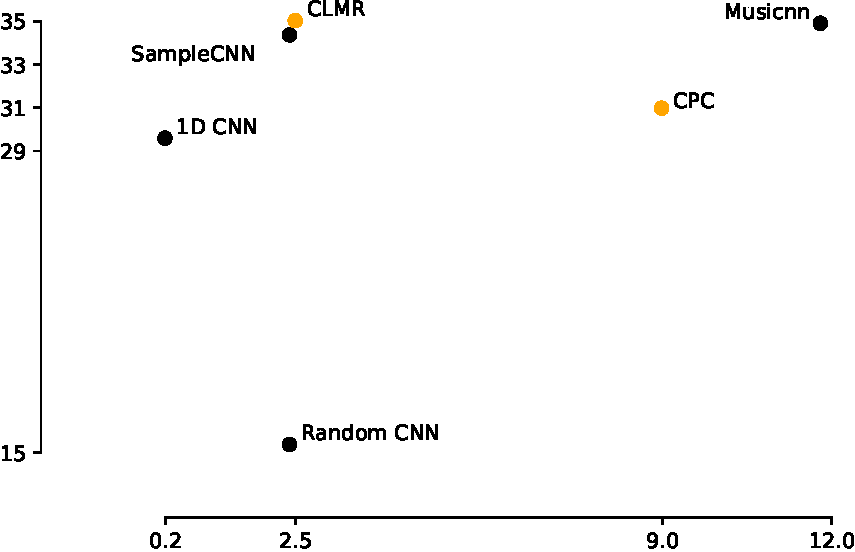
\includegraphics[width=0.75\columnwidth]{figs/roc_auc_magnatagatune.pdf}
    \caption{Performance and model complexity comparison of supervised models (grey) and self-supervised models (ours) in music classification of raw audio waveforms on the MagnaTagATune dataset to evaluate musical representations.
Supervised models were trained end-to-end, while CLMR and CPC are pre-trained without ground truth: their scores are obtained by training a linear classifier on their learned representations but nonetheless perform practically identically to the supervised models.}
    \label{fig:example}
\end{figure}

Self-supervised representation learning, a form of unsupervised learning, is a relatively new, upcoming learning paradigm \cite{dosovitskiy2015discriminative, oord_representation_2019, hjelm_learning_2019,chen_simple_2020}.
The general goal of representation learning is to train a function $g$ that maps input data $x \in \mathbb{R}^d$ to some representation of lower dimensionality, while preserving as much useful information as possible.
In the absence of ground truth, there can be no ordinary loss function for training $g$; self-supervised learning trains by way of a proxy loss function instead, obtained by withholding or augmenting parts of the input data.
One way to preserve the amount of useful information during self-supervised learning is to define the proxy loss function with respect to a relatively simple `pretext' task, with the idea that a representation that is good for the pretext task will also be useful for other tasks.
Many approaches simply rely on heuristics to design pretext tasks \cite{doersch_unsupervised_2015,zhang2016colorful}, e.g., by defining pitch transformation as a pretext task \cite{spice}.
Alternatively, \emph{contrastive representation learning} formulates the proxy loss directly on the learned representations and relies on comparing and contrasting multiple, slightly differing versions of any one example.
The rationale behind this contrastive strategy is \emph{predictive coding}, a theory that the human brain encodes causal structures and predicts future events at different levels of abstraction \cite{friston_predictive_2009}.


% may want to zoom out a bit, from 50 - 100 y-axis
% put in parenthesis [ours]
% square brackets citation
% add random baseline at 60% ROC
% add a labeled bracket that indicates the penalty / cost -> self-supervision penalty
% make the point of self-supervised learning this way

In this paper, we transfer the SimCLR framework \cite{chen_simple_2020} to the raw audio domain and contribute a pipeline of data augmentations on raw audio to form a simple framework for self-supervised, contrastive  learning of representations of raw audio waveforms.
To compare the effectiveness of this simple framework compared to a more complex self-supervised learning objective, we also evaluate representations learned by contrastive predictive coding \cite{oord_representation_2019}.
The models are evaluated on the downstream music tagging task, enabling us to evaluate their versatility: music tags describe many characteristics of music, e.g., genre, instrumentation and dynamics.
Our key contributions are summarized as follows.
\begin{itemize}
    \item CLMR achieves strong performance on the music classification task, despite self-supervised pre-training and fine-tuning on the downstream task using a linear classifier (see Figure~\ref{fig:example}).
    \item CLMR learns useful, compact representations from raw signals of musical audio.
    \item The learned representations are transferable across different musical corpora.
    \item CLMR can learn from \emph{any} dataset of raw audio, requiring neither transformations nor fine-tuning on the input data; nor do the models require manually annotated labels for pre-training.
    \item We provide an ablation study on the effectiveness of the data augmentations of raw audio.
\end{itemize}


\section{Outline}
In the following chapter, a comprehensive background of the field of self-supervised learning is be presented, as well as common neural network architectures in the raw audio domain.
Subsequently, the main downstream task and application of this thesis will be elaborated upon, along with its evaluation metrics.

In chapter 3, the method of this thesis is presented, outlining the details of the architecture of the model, its intuition, the objective function and the evaluation of the performance of the model.

In chapter 4, the implementation of the framework is discussed.

In chapter 5, the datasets are outlined, both for the main and transfer learning experiments.

In chapter 6, the results of this thesis are presented [...].

Lastly, the conclusions of this thesis are presented in chapter 9.


\chapter{Background}\label{sec:background}
In this chapter, we recapitulate the foundations which are used to build on in this work. In Section 2.1, we discuss the approaches to representation learning. In subsequent sections, we discuss an upcoming learning paradigm, self-supervised learning, the intuition and theory behind contrastive learning methods. In Section 2.4, we discuss convolutional neural networks for raw audio signals. In Section 2.5, we discuss the task of music auto tagging and their evaluation metrics.

\section{Representation Learning}
% The performance of machine learning models is heavily dependent on the choice of features and representations. These features are often engineered using human intuition and domain knowledge of the composition of the input data (i.e., feature engineering). While feature engineering can greatly help to improve model performance, it is time-consuming and highlights the inability of traditional learning algorithms to identify and disentangle explanatory factors hidden in high-dimensional signals. 

The goal of representation learning is to identify features that make  prediction tasks easier and more robust to the complex variations of natural data \cite{bengio2013representation}. Supervised techniques for representation learning have now been successfully applied to a variety of tasks \cite{korzeniowski_fully_2016, chen_harmony_2019, korzeniowski_end--end_2017, bock_joint_2016, pons_end--end_2017, van_den_oord_deep_2013}. 
% In the unsupervised domain, generative modeling and likelihood-based models use reconstruction of the observations as the objective for learning useful representations of the data. 
In unsupervised representation learning, generative modeling and likelihood-based models typically find useful representations of the data by attempting to reconstruct the observations on the basis of their learned representations \cite{goodfellow2014generative, unsupervised_gan}. Broadly speaking, these approaches can also be considered as self-supervised representation learning: the objective is formulated in such a way that it gets supervision from the data itself. The difference between generative approaches and self-supervised learning we like to distinguish, is that self-supervised learning aims to identify the explanatory factors of the data using an objective that is formulated with respect to the representations directly, and its goal is not to generate a faithful reproduction of the data but rather to learn useful features for (multiple) downstream tasks. \\

\section{Self-supervised learning}
This idea of self-supervised learning has seen widespread adoption in language modeling. Its most common task is to predict the next word, given a past sequence of words, but more auxiliary (pretext) tasks can be added to improve the language model. For example, BERT \cite{Devlin2019BERTPO} adds two auxiliary tasks that both rely on self-generated labels to improve the bi-directional prediction of word tokens and sentence-level understanding: 1) a cloze test \cite{doi:10.1177/107769905303000401}, in which part of the tokens in each sequence is randomly masked and the model is asked to predict the missing tokens, and 2) optimizing a binary classifier on predicting whether one sequence is the next one of another sequence. The first pretext task encourages the model to better capture the syntactic and semantic meaning of the context around a word, and the second task improves the understanding of relationships between sentences. Building these tasks requires no manual labeling, and can therefore be scaled up to arbitrary size while there is plenty of free text available to use as training data. \\

\subsection{Formulation of pretext tasks}
In the image domain, self-supervised learning manifests itself in a similar way: one or multiple pretext tasks are formulated on a set of unlabelled images and, subsequently, the pre-trained encoder or its intermediate layers are used to fine-tune on a downstream task like image classification. We give a short description of five different approaches. Exemplar-CNN \cite{dosovitskiy_discriminative_2014} creates a surrogate dataset by randomly applying a sequence of transformations to `exemplary' image patches that contain large gradients, e.g., image patches that contain edges, strong textures, i.e., objects or parts of objects of interest. Its pretext task is to classify the corresponding class of each transformed image. An even more simple pretext task is formulated in RotNet \cite{gidaris2018unsupervised}, that proposes to use a random 2d rotation transformation as a supervisory signal to learn semantic features of an image. The image is randomly rotated and given a class label: no rotation, $90^\circ$, $180^\circ$ or $270^\circ$, making the pretext task a 4-class classification problem. Arguably, this forces the model to learn relationships in the semantic space of objects, i.e., to recognize the same image under different rotations, it has to learn more high-level, structural parts of the image, e.g., the relative position of a nose with respect to the eyes. RotNet drastically reduced the gap between unsupervised and supervised feature learning in the image domain using a simple pretext task [TODO: scores here]. Another common transformation is that of colorization \cite{zhang_colorful_2016}, in which they extracted the lighting channel \textit{L} from a colored image and subsequently asked the model to predict the corresponding $a$ and $b$ color channels in CIE \textit{Lab} colorspace. A pretext task can also be formulated as a relationship between two random patches of a single image. In \cite{doersch2015unsupervised}, they exploit the spatial context of an image as a non-exhaustive, supervisory signal. Again given a large set of unlabeled images, random pairs of patches are extracted from each image and the network is asked to predict the position of the second patch relative to the first patch. A $3\times 3$ grid is constructed and, given the first patch is located in the center, the model is asked to predict the location of a patch located in any of the remaining 8 positions, turning the pretext task into an 8-class classification problem. In contrast to Exemplar-CNN, sampling is done without regard to the content of the image. Interestingly, this approach quickly found a trivial solution to the problem of identifying the relative position between a pair of images: chromatic aberration. This phenomenon arises when a lens fails to focus light at different wavelengths \cite{brewster_treatise_1835}. Convolutional neural networks are able to localise such patches relative to the lens, which makes the objective of identifying the relative position between two patches very easy to solve. While detailing more potential trivial solutions in the image domain is beyond the scope of this thesis, it is important to note that care must be taken for the model's ability to find trivial solutions to the problem when designing a pretext task. % In this case, the trivial solution was mitigated by shifting the green and magenta color channels to gray.
To conclude self-supervised learning in the image domain, \cite{noroozi_unsupervised_2016} converted aforementioned pretext task into a full $3\times 3$-grid `jigsaw puzzle', asking the model to reconstruct a sampled patch of an image after randomly shuffling all 9 sub-patches [TODO add a bit more detail why we include this].

From these series of approaches to self-supervised learning, we like to distinguish two categories of pretext tasks throughout this thesis: those that involve distortions to learn \textbf{spectral relationships} and and those that extract patches to learn \textbf{spatial relationships} in data. \\


Self-supervised learning on audio brings unique challenges compared to the image domain. Audio signals are high-dimensional, have a variable-length, and entail a hierarchical structure that is hard to infer without a supervisory signal. It is also highly variable, given different recording conditions, voice types, instrumentation, phonemes, syllables, etc. Work on self-supervised learning in audio was very limited at the beginning of this thesis. While it is still very limited in the music information retrieval field, several papers were published in the speech domain. PASE proposed a multi-task self-supervised learning approach, in which several workers each solved a self-supervised task for one neural encoder \cite{Pascual2019}. The learned representations were proven useful for speaker identity, phoneme and emotional cue recognition. During this thesis, PASE$+$ was published and improved on the latter method by adding random transformations to raw audio signals for more robust representations under noisy and reverberant environments \cite{Ravanelli2020}. It outperforms both PASE and encoders trained using common audio features, like MFCC's and filter banks. The workers in the PASE papers are small feed-forward neural networks and both solve self-supervised tasks. Common speech features are extracted from the audio, and are used as supervisory signals for the workers. These include regression workers that estimate log-power spectrum, MFCCs, prosody features, filter banks and their derivatives. Other workers are simple binary classifiers trained to maximize the mutual information between representations of positive and negative samples. The encoder and workers are jointly optimized using a loss function, which is formulated as the mean of workers' cost. Interestingly, the self-supervised learned features are also transferable: when trained on the LibriSpeech dataset, it achieves $74.1\%$ WER on the highly challenging CHiME-5 task\cite{barker2018fifth}. The series of transformations introduced in this paper will be further elaborated in section \ref{sec:audio_transformations}.

VQ-Wav2Vec

Contrastive predictive coding (CPC) was introduced as a universal approach to self-supervised learning, and has been successful for speaker and phoneme classification using raw audio, among other tasks in different domains \cite{oord_representation_2019}. It will be further detailed in Section \ref{sec:cpc}.

In music information retrieval specifically, recent advances have been made in self-supervised pitch estimation \cite{spice}, closely matching supervised, state-of-the-art baselines despite being trained without ground truth labels. Given a segment of raw audio, it scales the pitch of the signal, converts it to the time-frequency domain using a CQT transform as input data for a ConvNet encoder, and uses the scaling factor as a supervisory signal. To the best of our knowledge, SPICE\cite{spice} is the only (peer-reviewed) paper on self-supervised learning on audio in music information retrieval, and we are the first to perform self-supervised learning on raw audio waveforms of musical audio, without a transformation pipeline to the time-frequency domain, and evaluate the learned representations in a musical, downstream task.

\subsection{Ideal representations}
Aforedescribed pretext tasks are designed in a way they allow a model to learn representations that are not limited to solving the pretext task, but are also helpful in solving the downstream task when fine-tuning a classifier using the pre-trained intermediate layers. Ideal feature representations should be invariant to local translations and noisy variations of the input signal while remaing sensitive to higher-level semantic information. Put differently, the main challenge is to learn representations that effectively encode \textit{slow features} \cite{wiskott_slow_2002}, i.e., the shared information between parts of a high-dimensional signal. Conversely, a good representation should disregard noisy, more local features. The idea of slow features is quite intuitive for music.
We know that an audio fragment of a few seconds will share information with neighbouring fragments, e.g., the instrument(s) playing, the harmonic set of pitches or the identity of a vocalist.  But the further into the future a model is forced to predict these features, the less of this kind of shared information is available, thereby requiring the model to infer higher-level structure. Slow audio features span a longer temporal range (e.g., harmonic transitions or melodic contour) and are more interesting for use in downstream MIR tasks.


\subsection{Audio Augmentations}\label{sec:audio_transformations}
Earlier we distinguished two categories of pretext tasks: those that learn spectral relationships and spatial relationships. We can extend this intuition to data augmentations, as is done in Exemplar-CNN \cite{dosovitskiy_discriminative_2014} and PASE$+$ \cite{Ravanelli2020} as to create surrogate samples or learn more robust representations respectively. As described in the previous section, designing pretext tasks and augmentations in the audio domain brings unique challenges. We reckon one could resort to the time-frequency domain and use spectograms or CQT-transforms and treat them as visual input data, but one could argue that aforedescribed augmentations and pretext tasks have little to do with the spectral and spatial dynamics of an audio signal, e.g., randomly flipping a spectogram or applying color jitter to a CQT-transform has hardly anything to do with the original audio signal. We therefore describe several `spectral', i.e., acoustic augmentations that were introduced in the self-supervised speech representation learning literature \cite{Ravanelli2020} in Table \ref{tab:background_audio_augmentations}. Augmentations of musical data are motivated by the observation that learning algorithms may generalize better and learn more robust representations when trained on samples that are perturbed \cite{Sturm2015}. The augmentations introduced in the MUDA framework for musical data augmentations is further described in Table \ref{tab:background_music_augmentations}. In Chapter \ref{sec:method}, more audio augmentations will be discussed, which are used in the experiments of this thesis.

\begin{table}[h]
    \centering
    \resizebox{\columnwidth}{!}{
        \begin{tabular}{lllll}\toprule
        Augmentation & Details \\\midrule
        Reverberation & Convolution with a large set of impulse responses derived with the image method. \\
        Additive Noise & Non-stationary noises \\
        Frequency Masking & Convolution with band-stop filters, randomly dropping a spectrum band. \\
        Temporal Mask & Replace a random sequence of samples with zeros. \\ 
        Clipping & Add a random amount of saturation to simulate audio clipping conditions.  \\
        Overlapping & Overlap a random sample of audio to the current audio signal. \\
        \bottomrule
        \end{tabular}
    }
    \caption{Audio augmentations used in the speech domain to learn more robust representations using self-supervised learning methods.}
    \label{tab:background_audio_augmentations}
\end{table}


\begin{table}[h]
    \centering
    \resizebox{\columnwidth}{!}{
        \begin{tabular}{lllll}\toprule
        Augmentation & Details \\\midrule
        Pitch Shift & Shift the frequency of the signal by $n \in \{ -1, 0, +1 \}$ semitones. \\
        Time Stretch & Stretch the audio signal by a factor of $r \in \{ -2^{\frac{1}{2}}, 1, 2^{\frac{1}{2}} \}$ \\
        Background noise & Noise under three pre-recorded conditions is linearly mixed \\
        & with the input signal $y$, $\alpha$ being a random weight: $y^{\prime} \leftarrow(1-\alpha) \cdot y+\alpha \cdot y_{\text {noise }}$ \\
        Dynamic range compression & A common audio signal operation that both amplifies quiet \\
        & and reduces loud sounds, effectively reducing the signal's dynamic range. \\ 
        \bottomrule
        \end{tabular}
    }
    \caption{Musical audio augmentations from \cite{Sturm2015}}
    \label{tab:background_music_augmentations}
\end{table}




\section{Contrastive Learning}
In the following subsections, we highlight two frameworks for \textit{self-supervised} contrastive learning, which has recently received a lot of attention as a learning method in the self-supervised learning paradigm. First, the generic form of the objective of these learning methods is described.


\subsection{Contrastive Loss}
Its initial form as introduced by \cite{contrastiveloss}, the function runs over pairs instead of over individual samples. While loss functions closely related to contrastive learning were introduced like metric, margin and triplet loss \cite{8014803, marginloss, chechik_large_2009}, their differences lie in the sampling strategy for positive and negative samples. In supervised metric learning, the positive samples are chosen from the same class, while negative samples are chosen from different classes utilising hard-negative mining \cite{8014803}. In a triplet loss function, an input sample is compared to one positive and one negative sample. The choice of positive and negative samples in these losses are guided by the samples' corresponding labels in a supervised setting. Contrastive losses also rely on one positive pair, which can either be picked from neighbouring patches of the anchor sample, or an augmented version of the same data point. Different from the other loss functions, contrastive loss functions require many negative samples that are sampled from different data points. Inherently, it is assumed this reduces the probability of a false negative.


% It is insightful to consider the effects on the encoder due to minimizing Eq. 1. During training, for any i, the encoder is tuned to maximize the numerator of the log argument in Eq. 2 while simultaneously minimizing its denominator. The constraint that the term  is present in both the numerator and the denominator ensures that the log argument goes no higher than 1, and since Eq. 1 sums over all pairs of indices ((i, j) and (j, i)), the encoder is restricted from minimizing the denominator or maximizing the numerator without doing the other as well. As a result, the encoder learns to map similar views to neighboring representations while mapping dissimilar ones to non-neighboring ones.


\subsection{Contrastive Predictive Coding}\label{sec:cpc}
Contrastive predictive coding learns to predict representations of future observations from past observations. For audio, it predicts representations of segments of audio in the future. A sequential input signal $x_t$ is mapped by a non-linear encoder $g_{\mathrm{enc}}(\cdot)$ to a sequence of latent representations $h_t = g_{\mathrm{enc}}(x_t)$, while simultaneously an autoregressive model $g_{\mathrm{ar}}(\cdot)$ summarizes all encodings $h_{\leq t}$ in the latent space and maps them to a context latent representation $c_t = g_{\mathrm{enc}}(h_{\leq t})$. The vectors $h_t$ and $c_t$ are encoded so as to preserve maximal mutual information and to identify shared latent variables of the original signals: $g_{\mathrm{enc}}(\cdot)$ and $g_{\mathrm{ar}}(\cdot)$ jointly optimise InfoNCE, a contrastive loss based on noise-contrastive estimation \cite{gutmann_noise-contrastive_nodate}, and which has been widely used in previous work \cite{oord_representation_2019, sohn2020fixmatch, chen_simple_2020}. Given $N$ random samples from the set of encodings $X = \{h_{t+k}, h_{j_1}, h_{j_2} \hdots h_N\}$, $k$ being the number of timesteps the encoding occurs after $c_t$ and $X$ containing one positive sample $h_{t+k}$ and $N-1$ negative samples $h_{j_{n}}$ drawn from representations of other samples in the audio and dataset, the following objective is optimised:

\begin{equation}
    \mathcal{L}_{N}=-\sum_{k} \underset{X}{\mathbb{E}}\left[\log \frac{f_{k}\left(h_{t+k}, c_{t}\right)}{\sum_{h_{j} \in X} f_{k}\left(h_{j}, c_{t}\right)}\right]
\end{equation}

Each encoding pair $(h_n, c_t)$ is evaluated using a scoring function $f(\cdot)$ to estimate how likely a given $h_n$ is the positive sample $h_{t+k}$. CPC's formulation of the optimal solution for $f(\cdot)$ allows $-\mathcal{L}_n$ to be reformulated as a lower bound on the mutual information of representations $I(h_{t+k} | c_t)$, which also bounds the data $I(x_{t+k} | c_t)$, and is further proven by \cite{poole_variational_2019}. For downstream tasks, both $h_t$ and $c_t$ can be used as representations for new observations $x$, depending on whether context is helpful for solving it. Recently, the contribution of mutual information to the success of CPC has been reconsidered: its performance seems to depend largely on an inductive bias in the choice of a specialised architecture and the parameterisation of the mutual information critic \cite{Tschannen2020OnMI}.

% Contrastive predictive coding exploits this idea by learning representations that maximise mutual information among temporally neighbouring patches of data\cite{oord_representation_2019, hjelm_learning_2019}. 




\subsection{SimCLR}
SimCLR is a recently proposed contrastive learning technique for learning effective representations of images in a self-supervised manner without relying on specialised architectures and powerful autoregressive modeling \cite{chen_simple_2020}. The framework has four core components: 1) a composition of stochastic data augmentations that augment every image into two, correlated versions, 2) a ResNet encoder neural network, 3) a projector neural network and 4) a contrastive loss function, normalized temperature-scaled cross-entropy loss \cite{chen_simple_2020}.


\section{CNN's for Audio}

\subsection{SampleCNN}


\begin{table}[h]
    \centering
    \textbf{Convolution Block} \\
    \begin{tabular}{ccccc}
        \toprule Layer & Output Size \\\hline
        & (Sequence Length $\times$ Channels) \\
        Conv & h\_in $\times$ h\_out \\
        BatchNorm & h\_out \\
        ReLU & - \\
        \bottomrule
    \end{tabular}
    \caption{Convolution block consisting of a parameterised convolution layer and batch normalisation and ReLU activation layers.}
    \label{tab:conv_block}
\end{table}


\begin{table}[h]
    \centering
    \textbf{SampleCNN $3^9$ Model} \\
    \begin{tabular}{ccccc}
        \toprule Layer & Output Size & & Parameters & \\
        & (Sequence Length $\times$ Channels) & Kernel & Stride & Padding \\\hline
        Input & $59049 \times 1$ & 3 & 3 & 0 \\\hline
        ConvBlock & $19683 \times 128$ & 3 & 1 & 1 \\
        MaxPool & $6561 \times 128$ & 3 & 3 & 1 \\\hline
        ConvBlock & $6561 \times 128$ & 3 & 1 & 1 \\
        MaxPool & $2187 \times 256$ & 3 & 3 & 1 \\\hline
        ConvBlock & $2187 \times 256$ & 3 & 1 & 1 \\
        MaxPool & $729 \times 256$ & 3 & 3 & 1 \\\hline
        ConvBlock & $729 \times 256$ & 3 & 1 & 1 \\
        MaxPool & $243 \times 256$ & 3 & 3 & 1 \\\hline
        ConvBlock & $243 \times 256$ & 3 & 1 & 1 \\
        MaxPool & $81 \times 256$ & 3 & 3 & 1 \\\hline
        ConvBlock & $81 \times 256$ & 3 & 1 & 1 \\
        MaxPool & $27 \times 256$ & 3 & 3 & 1 \\\hline
        ConvBlock & $27 \times 256$ & 3 & 1 & 1 \\
        MaxPool & $9 \times 256$ & 3 & 3 & 1 \\\hline
        ConvBlock & $9 \times 512$ & 3 & 1 & 1 \\
        MaxPool & $3 \times 512$ & 3 & 3 & 1 \\\hline
        ConvBlock & $3 \times 512$ & 3 & 1 & 1 \\
        MaxPool & $1 \times 512$ & 3 & 3 & 1 \\\hline
        ConvBlock & $1 \times 512$ & 3 & 1 & 1 \\
        Dropout (0.5) & $1 \times 512$ & - & - & - \\\hline
        FC & 50 & - & - & - \\
        \bottomrule
    \end{tabular}
    \caption{SampleCNN $3^9$ Model, with 59049 samples (2678~ms) as input. Each ConvBlock consists of the modules presented in Table \ref{tab:conv_block}}
    \label{tab:samplecnn_model}
\end{table}


\section{Music Tagging}

\subsection{Evaluation Metrics}


\chapter{Method}\label{sec:method}
% We adapt and optimise the SimCLR framework for high-dimensional, raw signals of audio: Contrastive Learning of Musical Representations (CLMR).
\section{CLMR}
CLMR also consists of four core components, which will be elaborated further in the following subsections:
\begin{itemize}
    \item A stochastic composition of data augmentations that produces two correlated, augmented examples of the same audio segment, the `positive pair', denoted as $x_i$ and $x_j$.
    This is done for all segments in the mini-batch, resulting in $2N$ augmented examples per mini-batch.
    \item An encoder neural network $g_{\mathrm{enc}}(\cdot)$ that encodes the augmented examples to their latent representations.
    \item A projector neural network $g_{\mathrm{proj}}(\cdot)$ that maps the encoded representations to the latent space where the contrastive loss is formulated.
    \item A contrastive loss function, which aims to identify $x_j$ from the negative examples in the mini-batch $\{x_{k\neq i}\}$ for a given $x_i$.
\end{itemize}

The complete framework is visualised in Figure \ref{fig:clmr_model}.

\begin{fullwidth}
    \begin{figure*}[h]
        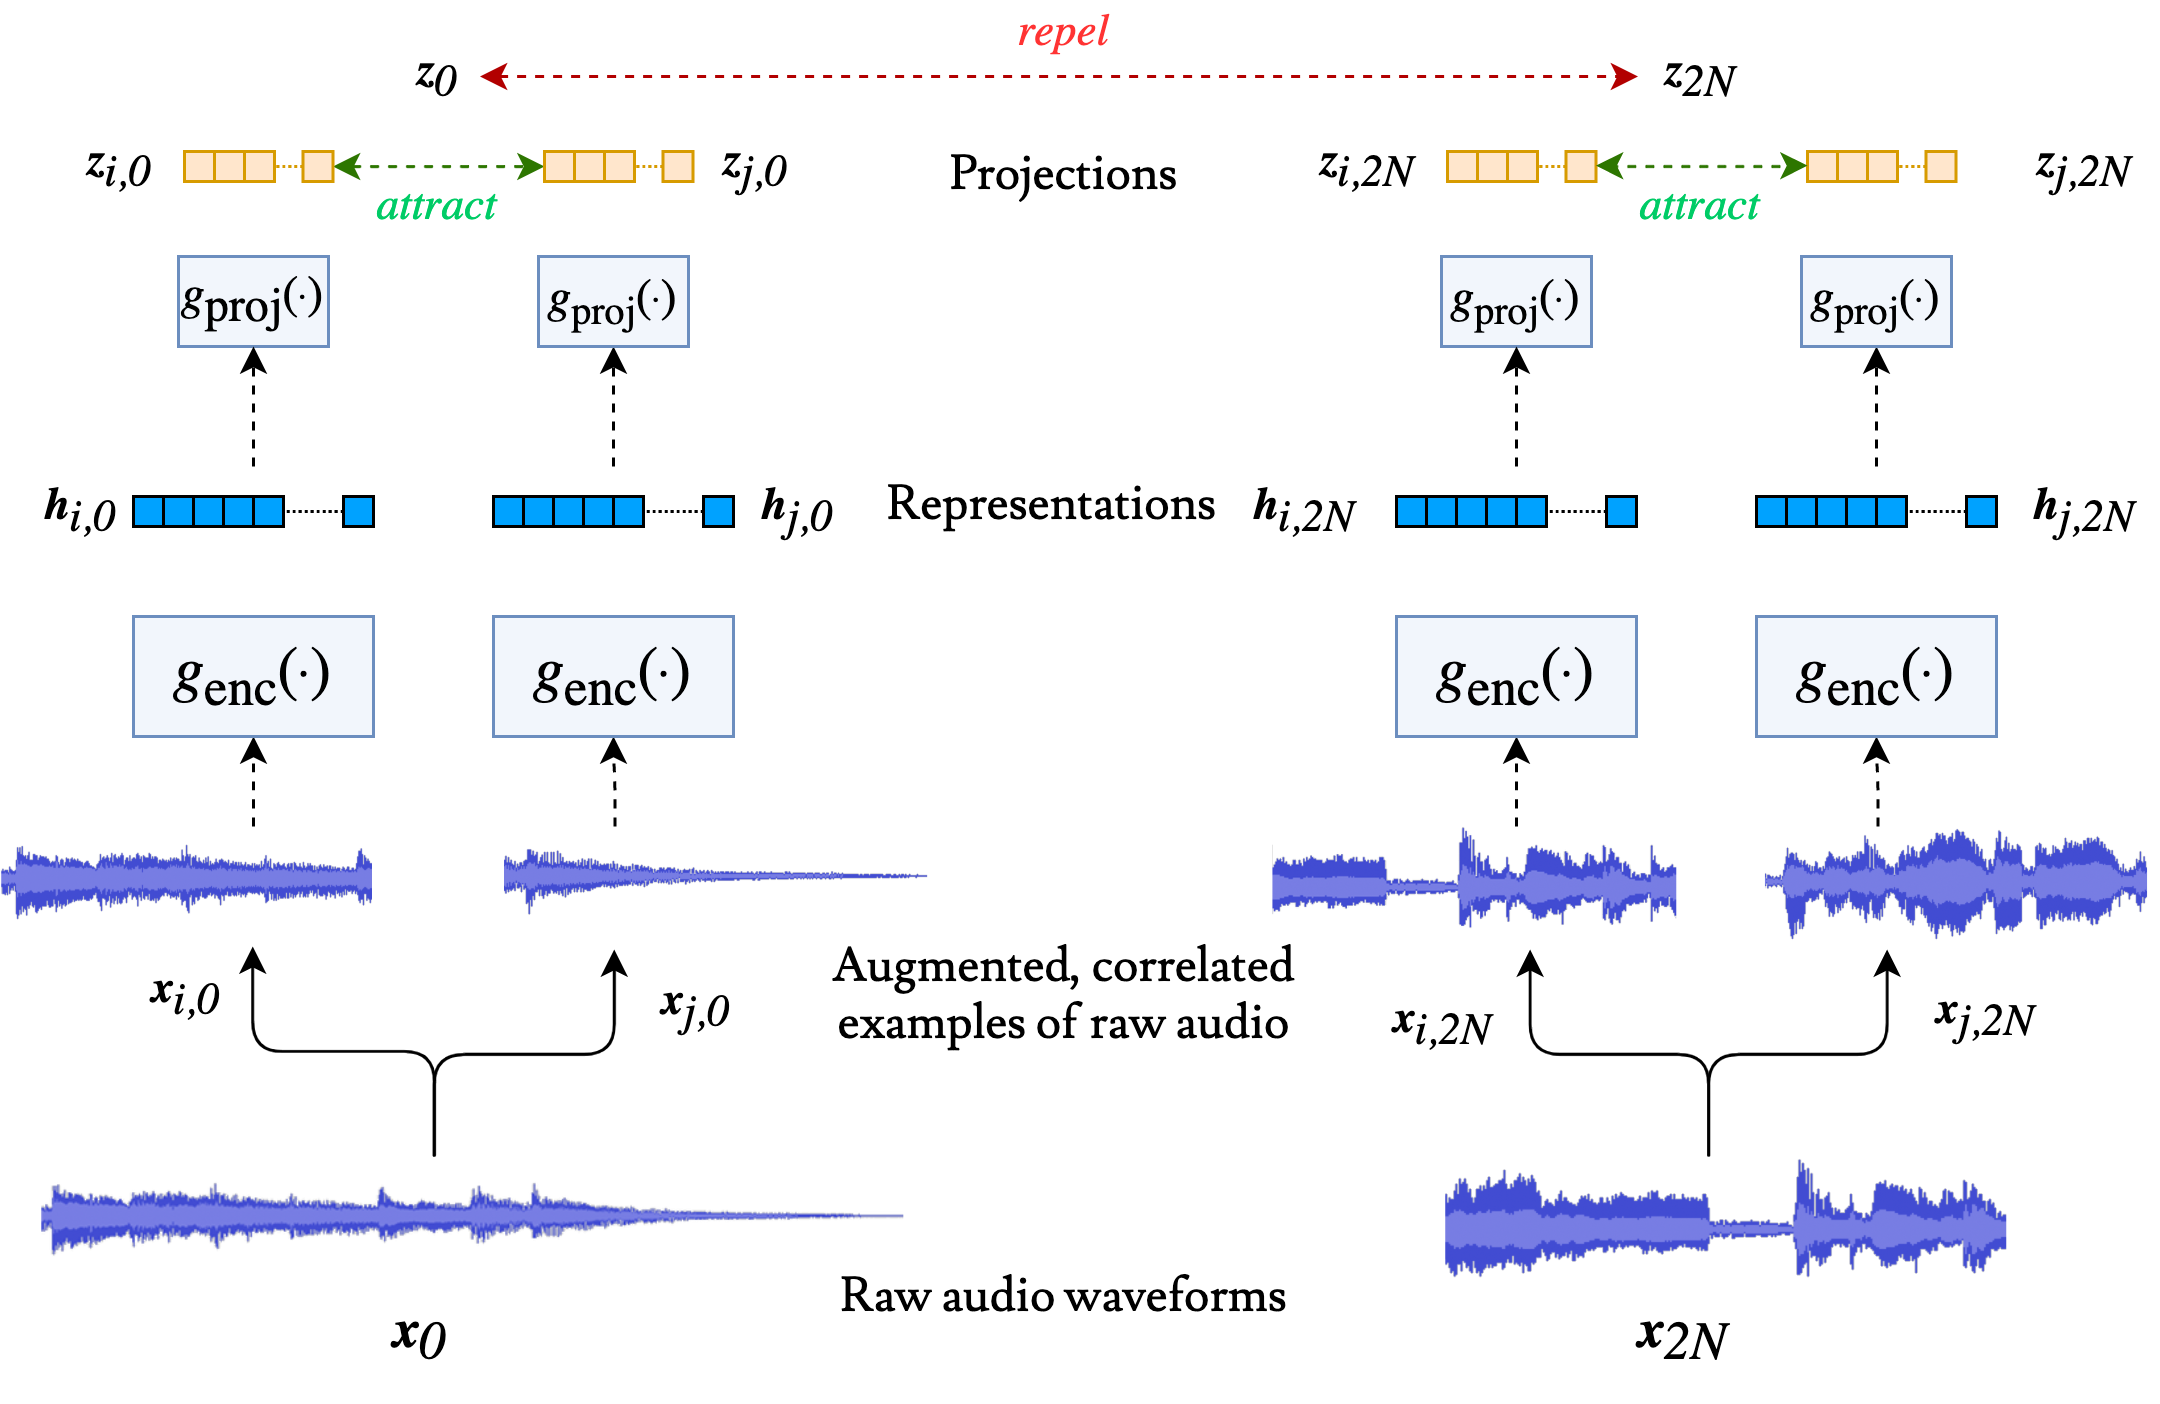
\includegraphics[width=\columnwidth]{figs/clmr_model.png}
        \caption{The CLMR framework operating raw audio, in which the contrastive learning objective is directly formulated in the latent space of correlated, augmented examples of pairs of raw audio waveforms.}
        \label{fig:clmr_model}
    \end{figure*}
\end{fullwidth}


\section{Data Augmentations}
We designed a chain of augmentations for raw audio waveforms to make it harder for the model to identify the correct pair of examples.
The following augmentations were applied on ${x_i}$ and ${x_j}$ independently:
\begin{enumerate}
    \item A random segment of size $N$ is selected from a full piece of audio, without trimming silence (e.g., the intro or outro of a song).
The independently chosen segments for $x_i$ and $x_j$ could overlap or be very disjoint, allowing the model to infer both local and global structures.
    \item The polarity is inverted, i.e., the amplitude is multiplied by $-1$, with probability $p_{\mathrm{invert}}$.
    \item Additive White Gaussian Noise is added with a high signal-to-noise ratio to the original signal with probability $p_{\mathrm{noise}}$.
    \item The gain is reduced between $[-6, 0]$ decibels with probability $p_{\mathrm{gain}}$.
    \item A filter is applied with probability $p_{\mathrm{filter}}$.
A coin flip determines whether it is a low-pass ($3500$~Hz) or high-pass ($800$~Hz) filter.
    \item The signal is delayed with probability $p_{\mathrm{delay}}$.
The delay time is randomly chosen from values between 200-500ms, with 50ms increments.
The volume factor of the delayed signal that is added to the original signal is 0.5.
    \item The signal is pitch shifted with probability $p_{\mathrm{pitch}}$.
The pitch transposition interval is drawn from a uniform distribution consisting of intervals ranging from a fifth below to a fifth above the original signal's scale.
    \item Reverb is added to the signal with probability $p_{\mathrm{reverb}}$.
The impulse response's room size, reverbation and damping factor is randomly chosen from a uniform distribution of values between $[0-100]$.
\end{enumerate}
The space of augmentations is not limited to these operations and could easily be extended to, e.g., randomly applying chorus, distortion and other modulations.


\section{Mini-Batch Composition} % Negative examples
We sample one song from the mini-batch, augment it into two examples, and treat them as the positive pair.
We treated the remaining $2(N-1)$ examples in the mini-batch as negative examples, and did not sample the negative examples explicitly.
A larger batch size makes the model's objective harder -- there are simply more negative samples -- but it can substantially improve model performance \cite{chen_simple_2020}.
This introduces a practical problem for raw audio when training on a GPU, as the input dimensionality of a raw waveform is higher for high sample rates.
The batch size can be increased more easily when audio is re-sampled at lower sampling rates: the number of examples the model is exposed to at once can be higher when the number of audio samples is lower.

Alternatively, multiple GPU's can be used for training, but this introduces another practical problem: batch normalisation \cite{batch_normalisation} is used in the encoder to stabilise training.
When training in a distributed, parallel manner, the batch normalisation statistics (mean/variance) are usually aggregated locally per device.
Positive examples are sampled on the same device, leading to potential leakage of batch statistics which improves training loss, but counteracts learning of useful representations.
We used global batch normalisation, which aggregates the batch statistics over all devices during parallel training, and leave the effect of different stabilisation strategies, e.g., layer normalisation \cite{henaff2019data}, for future work.


\section{Encoder}
Raw audio waveforms are very high-dimensional: a segment of 3 seconds already has 66\,150 samples when sampled at 22\,050~Hz, and they convey a lot of information at different time-scales.
The SampleCNN architecture, with its many convolutional layers with small filter sizes, has shown to capture these complexities very well for the task of music classification \cite{lee2018samplecnn}.
To directly compare an end-to-end supervised objective against a self-supervised objective, we use the SampleCNN model as our encoder.
Similar to the supervised approaches, we use an audio input of 59\,049 samples for audio with a sample rate of 22\,050~Hz.
In this configuration, the SampleCNN encoder $g_{\mathrm{enc}}$ consists of 11 blocks, each with a convolutional layer with a filter size of 3, batch normalisation, ReLU activation and max pooling with pool size 3.
The fully connected and dropout layers are removed, yielding a 512-dimensional feature vector for every sample of audio.
This feature vector is subsequently mapped to a different latent space by the projector network $g_{\mathrm{proj}}$ where the contrastive loss function is defined.
We adjust the audio input length and the encoder's blocks according to the configurations proposed in \cite{lee2018samplecnn} when training on audio sampled at different sampling rates (16\,000, 12\,000 and 8\,000~Hz).

% There is a trade-off between the number of contrastive examples the model is exposed to at once, and model complexity: increasing both quickly results in hardware constraints for training (GPU memory).
We found working with a batch size of 48 and a $3^9$-SampleCNN encoder to work well and easier to compare with against related work using supervised methods \cite{lee2018samplecnn, dieleman2014end,pons_end--end_2017}.
We leave model scaling for future work.


\section{Projector}
The feature vectors from the encoder can be directly used in the learning objective, but SimCLR shows that formulating the objective on encodings mapped to a different latent space by a parameterised function helps the effectiveness of the representations \cite{chen_simple_2020}.
We evaluate the performance improvement when using a linear layer $z_i = Wh_i$, non-linear layer $z_i = W^{(2)}\operatorname{ReLU}(W^{(1)}h_i)$ and an identity function $z_i = h_i$ as the projector.
% \diffword{Layer2 is data augment in \ref{clmr}}.


\section{Contrastive Loss Function}
In keeping with recent findings on several objective functions in contrastive learning \cite{chen_simple_2020}, the contrastive loss function used in this model is normalised temperature-scaled cross-entropy loss, commonly denoted as \emph{NT-Xent loss}:
\begin{equation}
    \label{ntxent_loss}
    \ell_{i, j}=-\log \frac{\exp \left(\operatorname{sim}\left(z_{i}, z_{j}\right) / \tau\right)}{\sum_{k=1}^{2 N} \mathbbm{1}_{[k \neq i]} \exp \left(\operatorname{sim}\left(z_{i}, z_{k}\right) / \tau\right)}
\end{equation}
%, demonstrated for a single pair in equation \ref{ntxent_loss}.

Instead of using a scoring function that preserves the mutual information between vectors, the pairwise similarity is measured using cosine similarity ($\operatorname{sim}$).
% : $f(\cdot) = \operatorname{sim}(\boldsymbol{u}, \boldsymbol{v})=\boldsymbol{u}^{\top} \boldsymbol{v} /\|\boldsymbol{u}\|\|\boldsymbol{v}\|$.
It introduces a new temperature parameter $\tau$ to help the model learn from hard negatives.
The indicator function $\mathbbm{1}_{[k \neq i]}$ evaluates to $1$ iff $k\neq i$.
% ref to figure
This loss is computed for all pairs, both $(z_i, z_j)$ and $(z_j, z_i)$, resulting in the following total loss function:
% shown in equation \ref{total_xent_loss}.

\begin{equation}
    \label{total_xent_loss}
    \mathcal{L} = \frac{1}{2N}\sum_{i=1}^{N}\sum_{j=1}^{N} \mathbbm{1}_{[i\neq j]}\ell_{i, j}
\end{equation}

We used the Adam optimizer \cite{adam_optimizer} with a learning rate of $3\times10^{-4}$ and train until convergence.


\section{Evaluation}
\label{evaluation}
The evaluation of representations learned by self-supervised models is commonly done with linear evaluation \cite{oord_representation_2019,hjelm_learning_2019,chen_simple_2020}, which measures how linearly separable the relevant classes are under the learned representations.
We obtain representations $h_t$ for all data points $X$ from a frozen CLMR network after pre-training has converged, and train a linear classifier using these self-supervised representations on the downstream task of music classification.
For CPC, the representations are extracted from the autoregressor, yielding context vector $c$ of $256$ dimensions, which is global-average pooled to obtain a single vector of $512$ dimensions.
For CLMR, the representations $h$ from the encoder are used instead of the representations $z$ from the projector.


\section{Transfer Learning}
To test the generalisability of the learned representations, we also pre-trained CLMR on different datasets than those we use for evaluation.
We pre-train CLMR on the Million Song Dataset, freeze the weights of the network, and subsequently process all datapoints $X$ from the smaller MagnaTagATune dataset to obtain representations $h$, on which we perform the same linear evaluation procedure outlined in the previous paragraph.


% \section{Implementation}

% \subsection{Contrastive Predictive Coding}
% We adjusted the original CPC encoder $g_{\mathrm{enc}}$ to a deeper architecture, as previous work \cite{lee2018samplecnn} shows more convolutions with smaller filter sizes helps to learn more useful representations of musical audio.
The encoder $g_{\mathrm{enc}}$ consists of 7 layers with 512 filters each, and filter sizes $[10, 6, 4, 4, 4, 2, 2]$ and strides $[5, 3, 2, 2, 2, 2, 2]$.
This results in a downsampling factor of $490$, which yields a feature vector for every $\approx$ 5~ms of audio for an input of 59\,049 samples.
Instead of relying on max-pooling, the filter sizes and strides are adjusted accordingly to parameterise and facilitate downsampling.
We also increased the number of prediction steps $k$ to 20, effectively asking the network to predict 100~ms of audio into the future.
The mini-batch size, i.e., the number of training examples the model is exposed to at once, is set to 64 from which 15 negative samples in the contrastive loss are drawn.

\chapter{Datasets}

\begin{quote}
    In this chapter, we first give a short background on the standardisation of datasets and evaluation procedures in the field of MIR. Then, we give a more detailed description of the datasets that were used for the experiments in this thesis.
\end{quote}

We used the MagnaTagATune dataset and Million Song Dataset \cite{Bertin-Mahieux2011} for pre-training and evaluation.

For the transfer learning experiments, we pre-train CLMR on the Million Song Dataset, fault-filtered GTZAN \cite{tzanetakis2002musical,sturm2013gtzan}, McGill Billboard \cite{burgoyne_billboard} and Free Music Archive \cite{fma_dataset} datasets.
We subsequently perform linear evaluation of the self-supervised learned representations on the MagnaTagATune dataset.

\section{MIREX}
There are several benchmark datasets that are used to evaluate music classification algorithms with.
One of the first attempts to unify datasets and evaluation procedures for music (classification) algorithms is MIREX: the Music Information Retrieval Evaluation eXchange.
This `exchange' was started as a platform to evaluate newly published algorithms on many tasks in the field of MIR.
The MIR tasks range from chord recognition, music key detection, audio fingerprinting to music classification.
Along with the unification of evaluation procedures, it has also produced standard datasets to benchmark algorithms with.
For the task of music classification, the MagnaTagATune dataset \cite{law2009evaluation} is often used.
For chord recognition, the Billboard dataset is regarded as a standard dataset \cite{burgoyne_billboard}.


\section{MagnaTagATune Dataset}
The MagnaTagATune dataset was compiled by crowdsourcing tags from a game called `TagATune' using music from the Magnatune label.
For the MagnaTagATune dataset, we used the original, MIREX 2009 version, consisting of 25\,863 songs, and the same dataset split, so that we can compare our results with previous work easily \cite{pons_end--end_2017, lee2018samplecnn, dieleman_feature_learning}.
It should be noted that this original version contains tag labels that are synonymous, e.g., `female', `woman', `no vocal', `no voice' and also contains tracks that do not have any labels. The top-50 tags in the MagnaTagATune dataset are shown in Table \ref{tab:magnatagatune_tags}.

The distribution of the number of fragments per class is skewed: there are more fragments containing guitar and classical tag attributes than `country' or `harp' attributes. A possible consequence of this class imbalance, is that CLMR learns representations that separate, e.g., `guitar' music and `flute' music well, but it is harder to learn representations that separate `country' music from `choral' music.


\begin{figure}
    \centering
    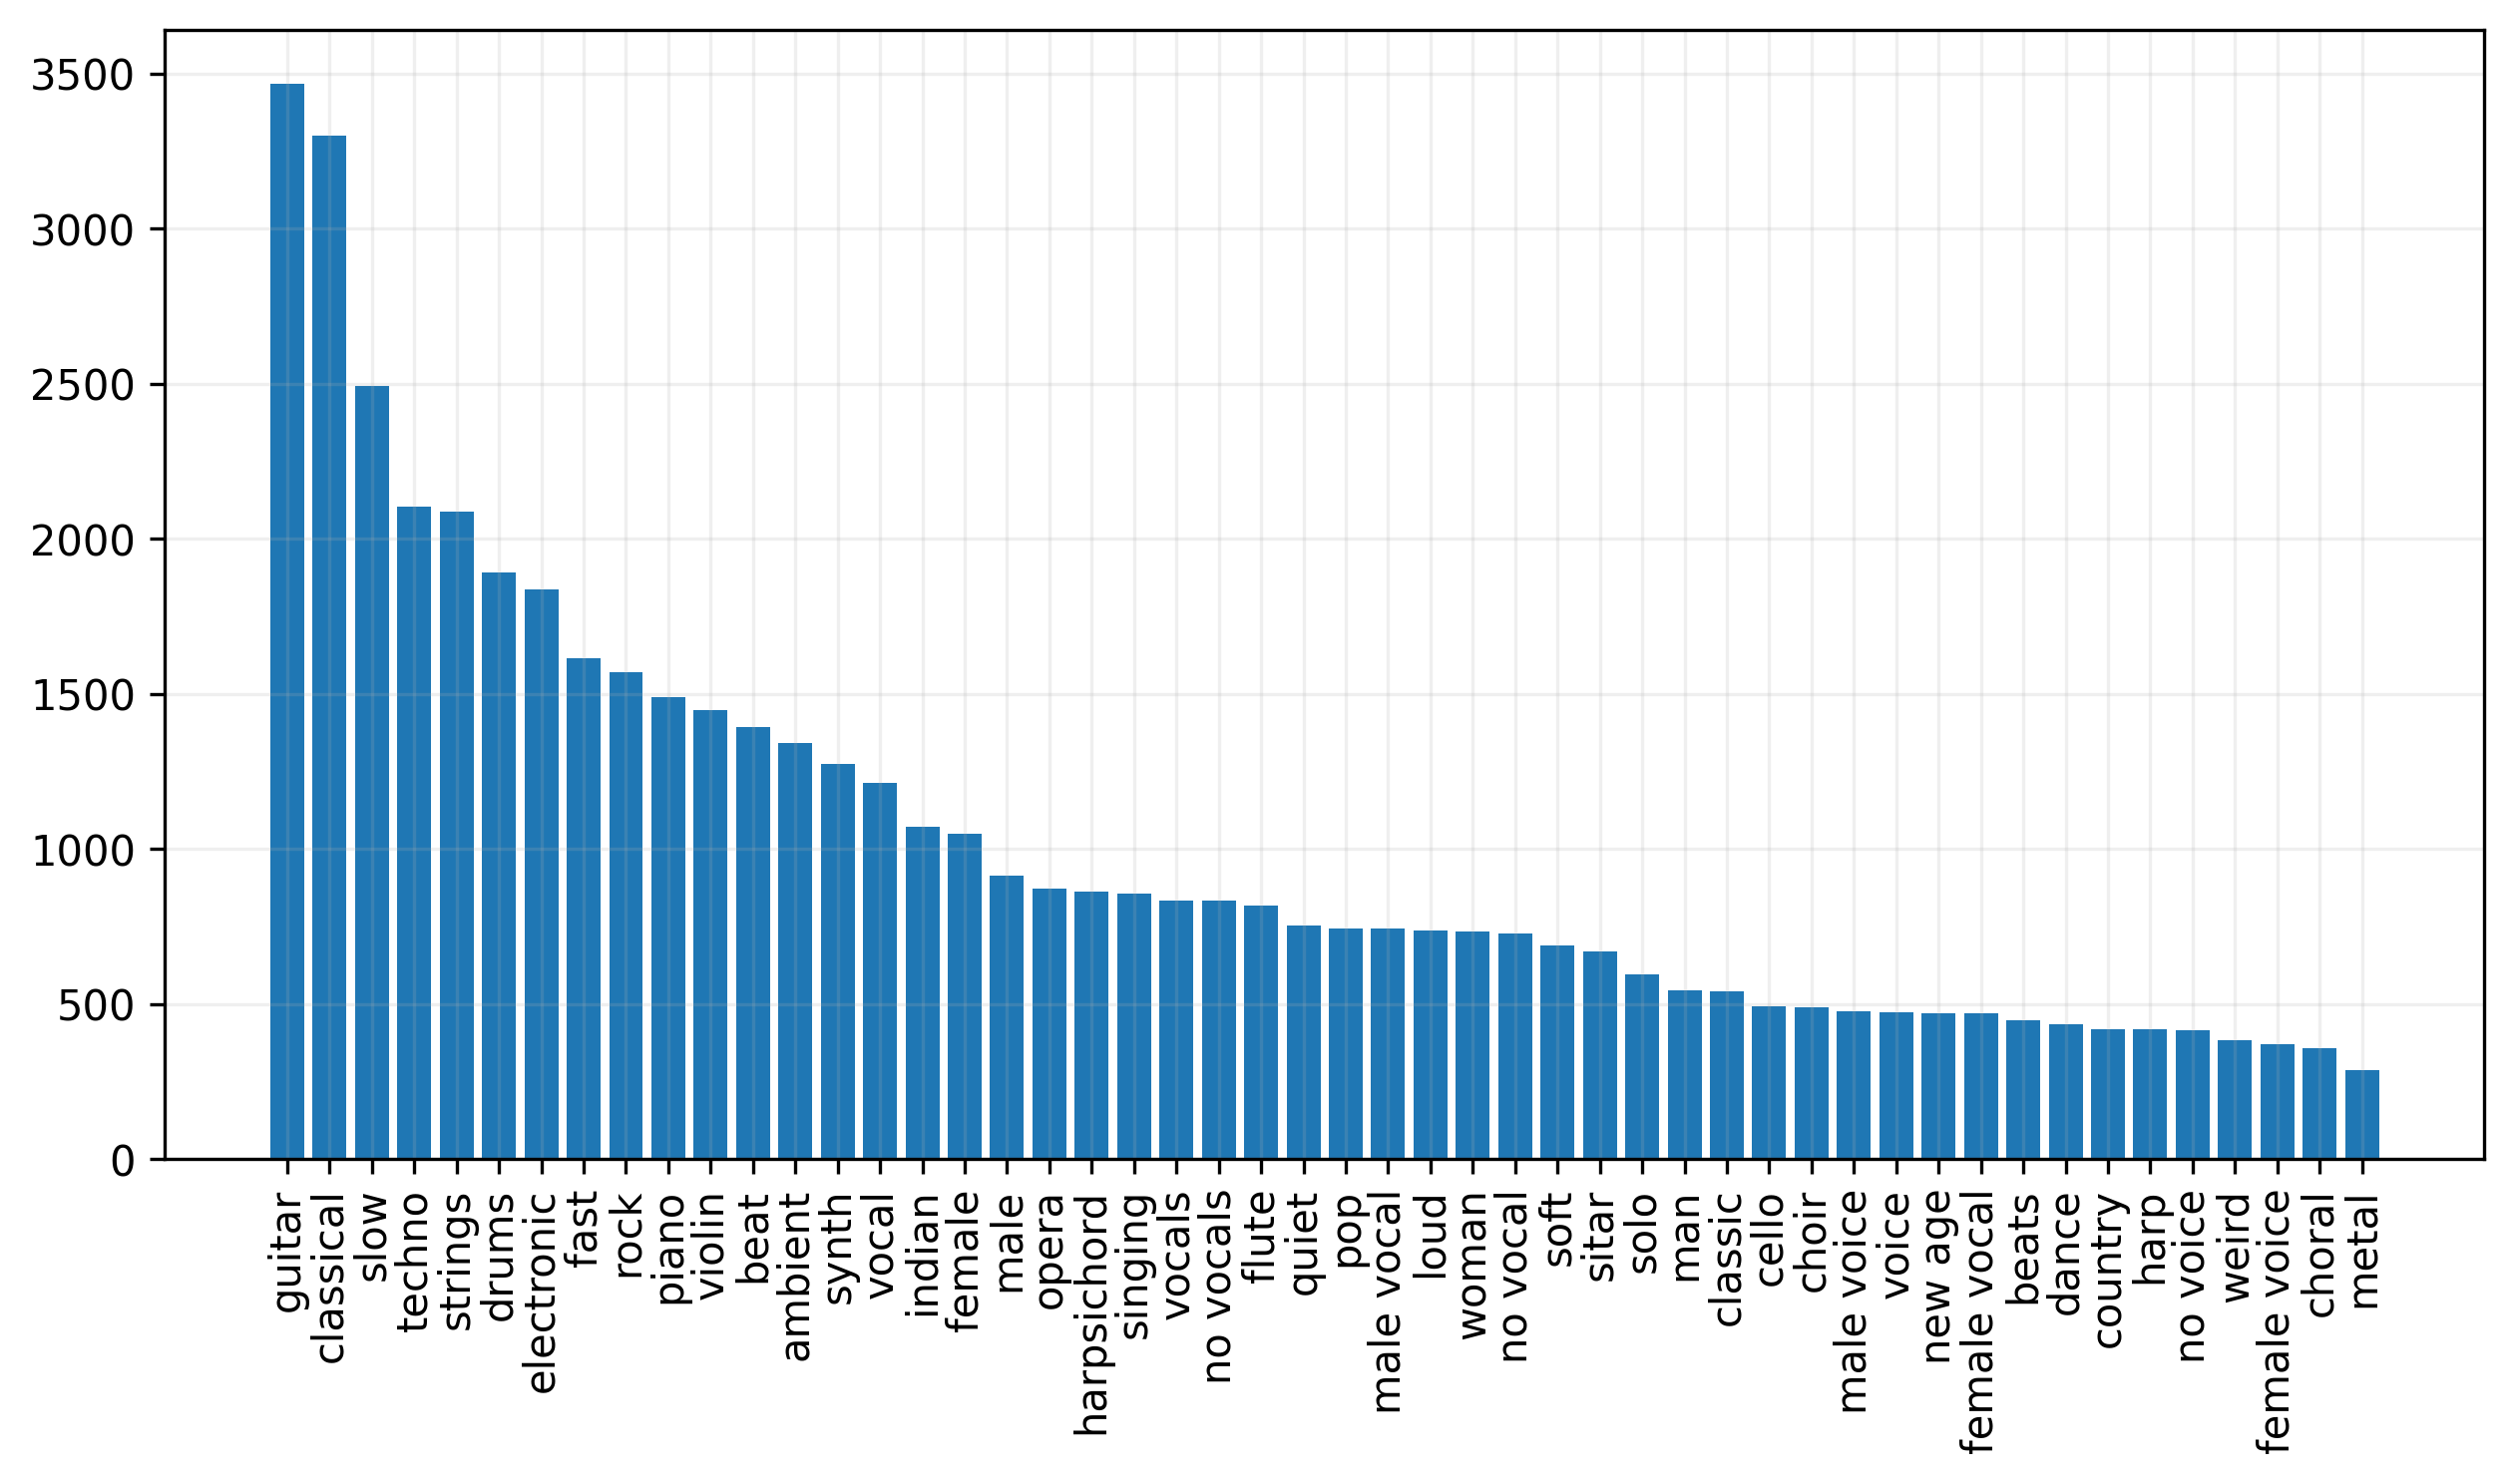
\includegraphics[width=\columnwidth]{figs/tag_stats_magnatagatune.png}
    \caption{Distribution of tags of the MagnaTagATune dataset}
    \label{fig:tag_stats_magnatagatune}
\end{figure}


\begin{table}[t]
    \centering
    \begin{tabular}{lll}\toprule
        guitar  & classical & slow \\
        techno & strings & drums \\
        electronic & rock & fast \\
        piano & ambient & beat \\
        violin & vocal & synth \\
        female & indian & opera \\
        male & singing & vocals \\
        no vocals & harpsichord & loud \\
        quiet & flute & woman \\
        male vocal & no vocal & pop \\
        soft & sitar & solo \\
        man & classic & choir \\
        voice & new age & dance \\
        male voice & female vocal & beats \\
        harp & cello & no voice \\
        weird & country & metal \\
        female voice & choral & \\                 
        \bottomrule
    \end{tabular}
    \caption{50 most popular tags in the MagnaTagATune dataset}
    \label{tab:magnatagatune_tags}
\end{table}



\section{Million Song Dataset}
The Million Song Dataset consists of 1 million audio features and metadata of contemporary pop songs.
It is commonly used for benchmarking on a larger scale.
These features were compiled by The Echo Nest, a music data company that has since been purchased by Spotify.
While they provide the audio features that are computed using their proprietary algorithms, the raw audio data is not provided due to the infringement of copyright when published freely and publicly.

Since this thesis uses raw audio to train and evaluate the CLMR model on, it was a challenge to obtain the raw audio of the contempory pop songs.
Originally, it could be obtained by accessing 30-second fragments using the internal IDs matched with those from the `7 digital' music service.
\footnote{\url{7digital.com}}
Since it does not provide this service anymore, we had to obtain the dataset from a another MIR research group that archived the 7digital fragments.
\footnote{We would like to thank Jongpil Lee from the Korea Advanced Institute of Science and Technology for providing us access to their server to retrieve the 30-second raw audio fragments.}

The Million Song Dataset's tags were compiled by cross-referencing it with the crowdsourced Last.fm dataset \cite{Bertin-Mahieux2011}. Similar to the MagnaTagATune dataset, we use only tracks that were annotated with tags from the set of top-50 most popular tags. This results in $241,904$ unique songs.

The tags for the Million Song Dataset are more overlapping, e.g., `rock' and `classic rock', and contain more semantic tags, e.g., `beautiful', `happy' and `sad', which are arguably harder to linearly separate when fine-tuning the linear classifier.
The top-50 tags are shown in Table \ref{tab:msd_tags}. Similar to the MagnaTagATune dataset, the classes are also imbalanced in this dataset. 
The `rock' attribute is overrepresented in the dataset.
While we did not correct for this imbalance, we reckon it has a similar effect on the learned representations as described earlier for the MagnaTagATune dataset.


\begin{figure}
    \centering
    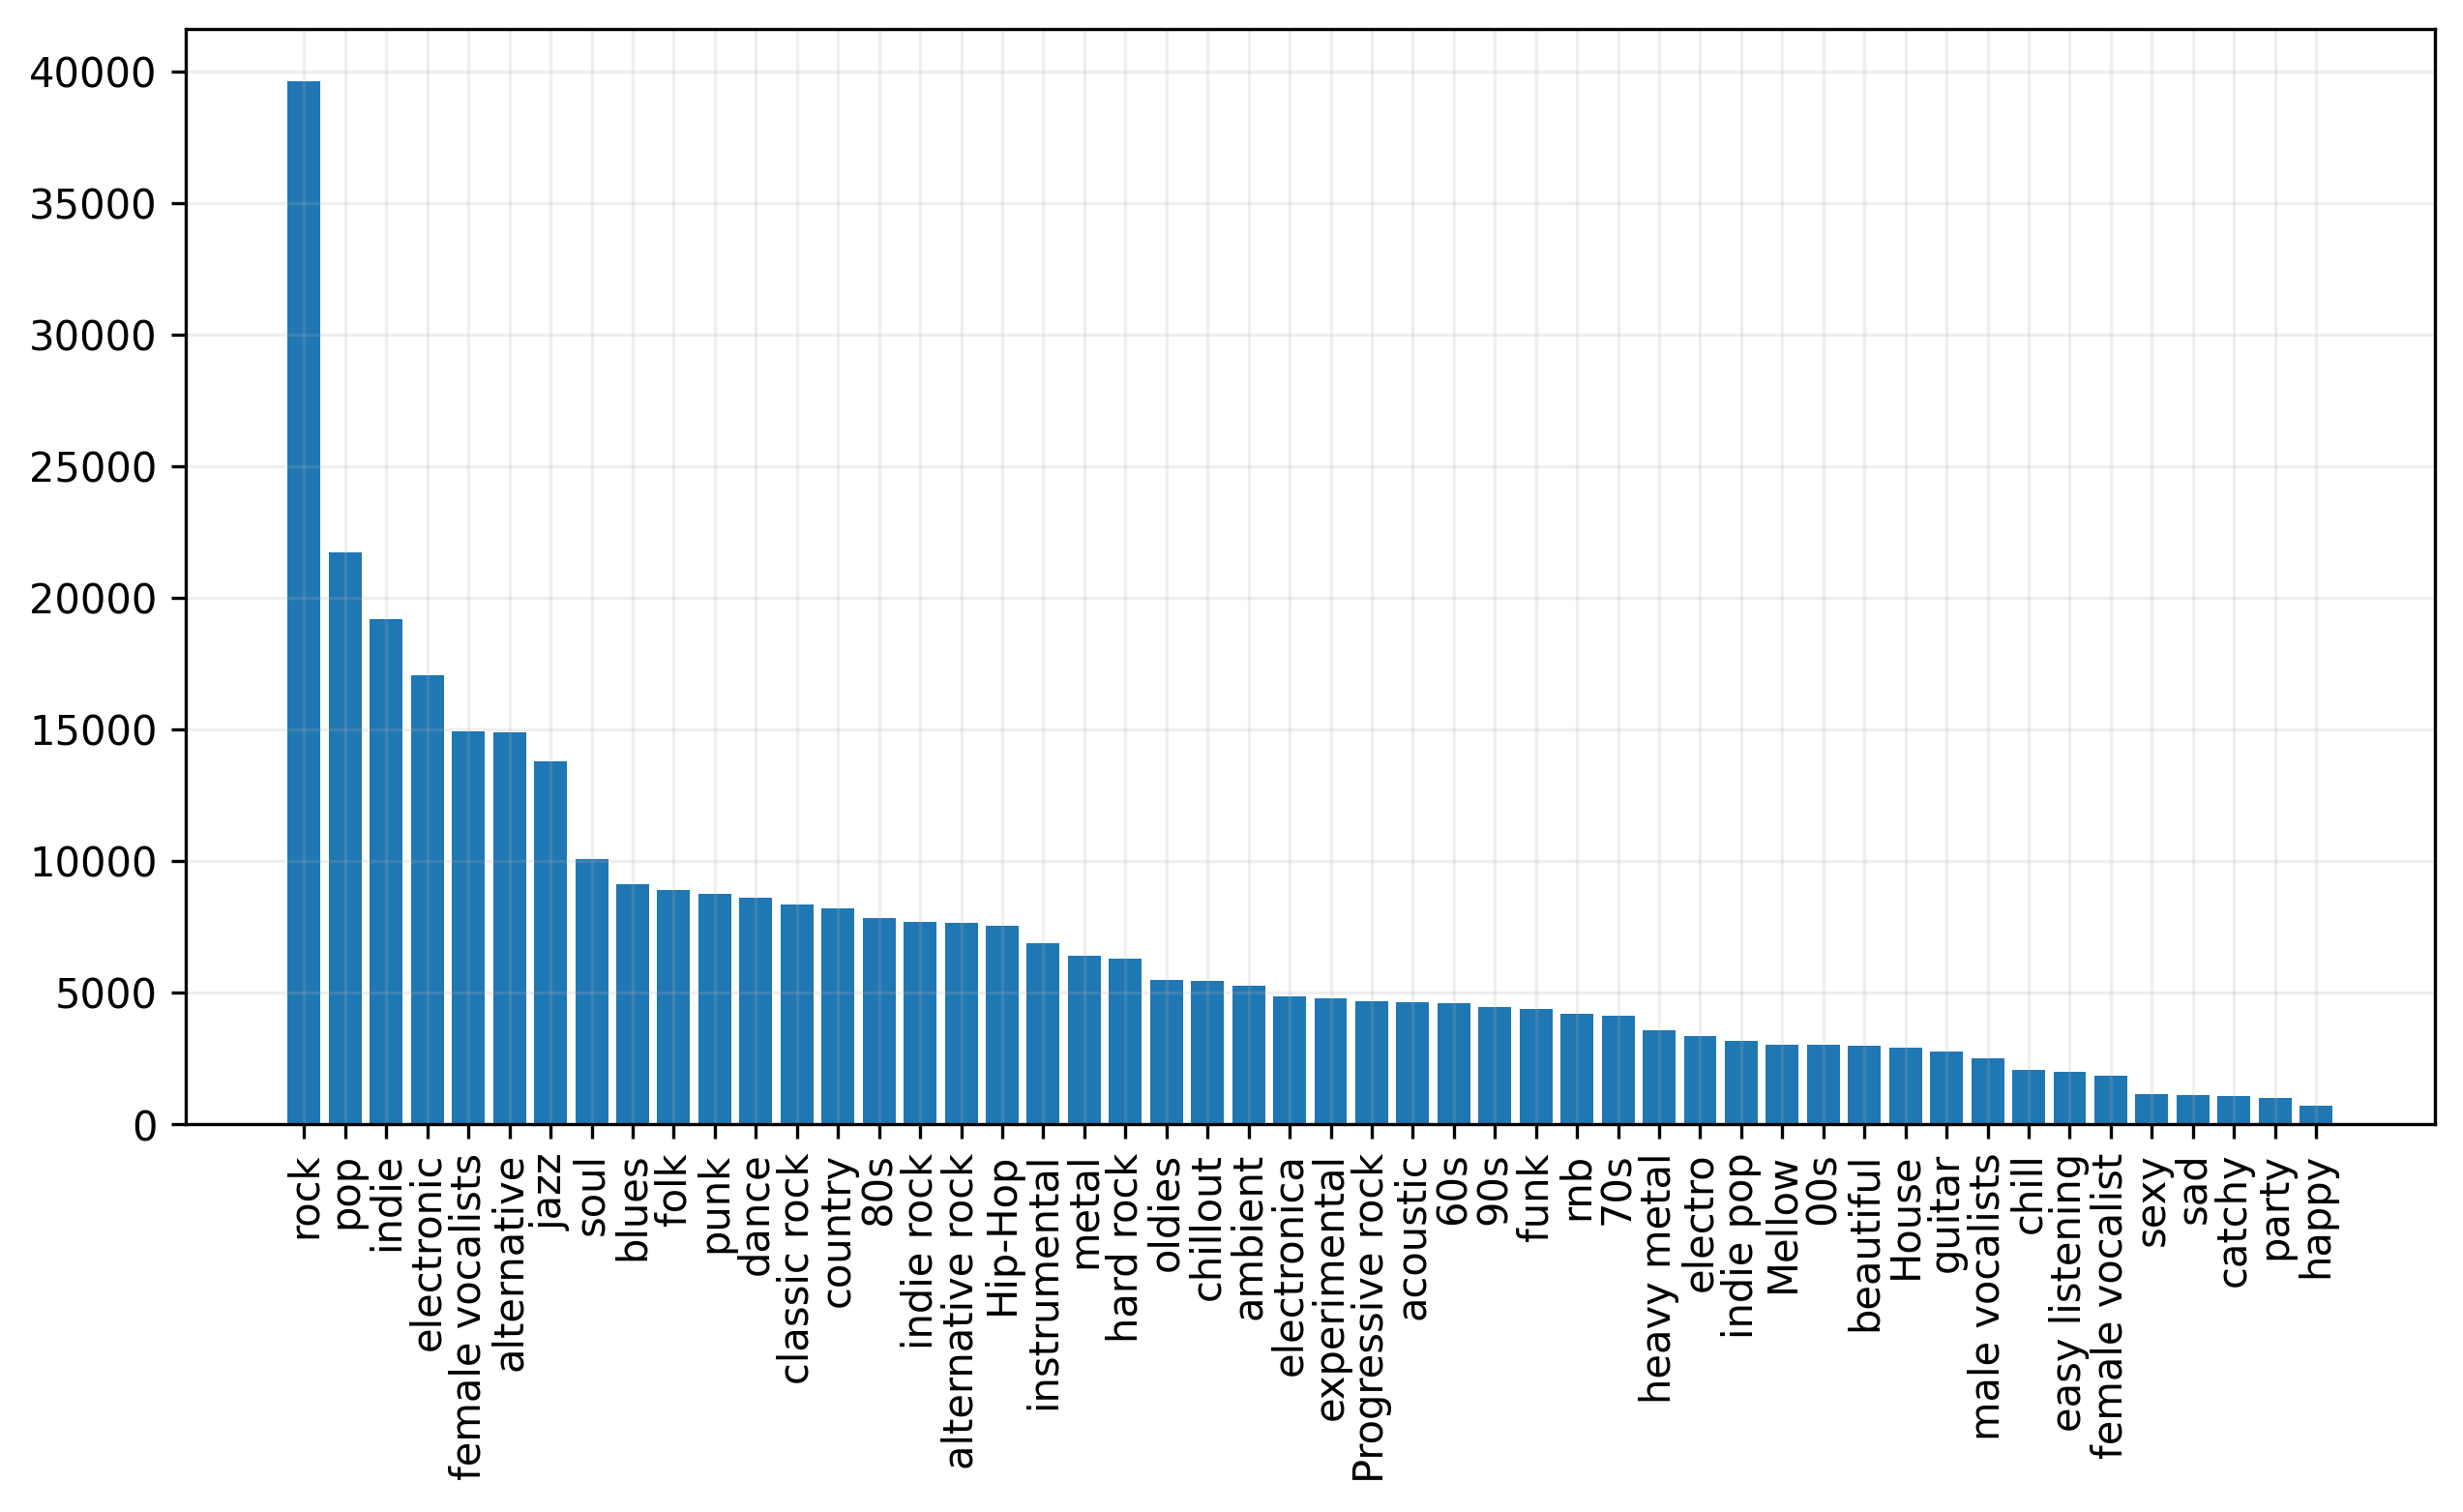
\includegraphics[width=\columnwidth]{figs/tag_stats_msd.png}
    \caption{Distribution of tags of the Million Song Dataset}
    \label{fig:tag_stats_msd}
\end{figure}


\begin{table}[t]
    \centering
    \begin{tabular}{lll}\toprule
        rock & pop & alternative \\
        indie & electronic & female vocalists \\
        dance & 00s & alternative rock \\
        jazz & beautiful & metal \\
        chillout & male vocalists & classic rock \\
        soul & indie rock & mellow \\
        electronica & 80s & folk \\
        90s & chill & instrumental \\
        punk & oldies & blues \\
        hard rock & ambient & acoustic \\
        experimental & female vocalist & guitar \\
        hip-hop & 70s & party \\
        country & easy listening & sexy \\
        catchy & funk & electro \\
        heavy metal & progressive rock & 60s \\
        rnb & indie pop & sad \\
        house & happy & \\
        \bottomrule
    \end{tabular}
    \caption{50 most popular tags in the Million Song Dataset}
    \label{tab:msd_tags}
\end{table}



% Like the other studies, we use average tag-wise ROC-AUC and PR-AUC scores as evaluation metrics, which are global measures indicating how well the classifier ranks segments given a tag.
% PR-AUC is calculated in addition to ROC-AUC because ROC-AUC scores can be over-optimistic for imbalanced datasets like Magna\-Tag\-A\-Tune.


\section{Transfer Learning Datasets}
\subsection{McGill Billboard Dataset}
From the McGill Billboard dataset, we use 461 audio files of contemporary pop songs for training.
While this dataset is most often used for evaluating chord recognition algorithms, we use the audio solely for self-supervised pre-training. The audio is only used for self-supervised pre-training.

\subsection{Free Music Archive}
Similarly, we use the Free Music Archive dataset, consisting of 22\,413 unique multi-labeled songs for the `medium' version, 

\subsection{GTZAN}
The fault-filtered GTZAN dataset contains 930 segments of 30 seconds, each having a single label denoting its genre \cite{Sturm2015, tzanetakis2002musical}. The dataset is made up of 10 genres: classical, country, disco, hip-hop, jazz, rock, blues, reggae, pop and metal. The audio is again only used for self-supervised pre-training.


\chapter{Implementation}
\begin{quote}
    In this chapter, we give a comprehensive overview of the implementation of the CLMR model. We provide a PyTorch \cite{pytorch2019} implementation for both CLMR and CPC. The code implementation can be found on GitHub.\footnote{\url{https://github.com/spijkervet/CLMR}}
\end{quote}


\section{CLMR}
The CLMR model extends the vision contrastive learning framework, SimCLR \cite{chen_simple_2020}. We implemented their paper in PyTorch and ran extensive experiments to ensure it met the original paper's results.
We provide the code on GitHub as well.
\footnote{With 250+ stars and 50+ forks, our code has grown into one of the most popular PyTorch implementations of this framework: \url{https://github.com/spijkervet/SimCLR}}
\footnote{After we published the code, the original author, Ting Chen, also published their implementation in TensorFlow. We are cited as one of the PyTorch implementations in their work \url{https://github.com/google-research/SimCLR}}

\subsection{Optimising Audio Transformations}
The data augmentation pipeline consists of functions from the following code libraries:
\begin{verbatim}
    essentia
    torchaudio
    librosa
    sox
    wavaugment
\end{verbatim}
We use large mini-batch sizes for training, and while every mini-batch must contain randomly augmented examples, it is of significant importance to optimise the runtime of a parallelised augmentation pipeline.
Since audio transformations are CPU-intensive operations, most libraries have optimised their code by creating an interface between Python and languages that map their code more efficiently to machine instructions, e.g., the C language, to avoid a bottleneck on these augmentations.
\footnote{Python is an interpreted language, which makes it slower than machine code because making interpretations of instructions takes longer than executing machine instructions directly.}
However, both pitch-shifting and reverberation have not yet been fully optimised for Python. The code implementation of WavAugment provides a Python - C++ interface to interact with all audio effects in the sox library from within Python \cite{wavaugment2020}.
We use this implementation to significantly speed up pitch-shift and reverberation transformations in our augmentation pipeline.

\subsection{GPU Parallelisation}
PyTorch provides two interfaces to parallelise training on GPU's.
This can be used to either scale up the model, i.e., by increasing the number of parameters or by increasing the mini-batch size, or to speed up training.
The `DataParallel' (DP) module parallelises the data across multiple GPU's on a single node, while `DistributedDataParallel' (DDP) distributes it over multiple GPU's across multiple nodes.
We use either DP or DDP to speed up training or to increase the mini-batch size.
The maximum available hardware provided for this thesis was a a single $4\times \text{Titan RTX}$ node with 96 gigabytes of GDDR6 memory.
\footnote{We would like to thank SURFsara for providing the GPU nodes on the lisa system.}
This allowed us to train our best-performing model with a mini-batch size of 456. For future work, this can be scaled even more if more hardware is available.

As described earlier, batch normalisation is used in the convolution block to stabalise training, especially for larger mini-batch sizes \ref{tab:conv_block}.
Since information about batch statistics could leak to the learning objective, we utilise global batch normalisation.
It aggregates the operation from the devices to a single GPU device, and subsequently distributes the results to the other devices.

For multi-node training using DDP, the losses from all devices need to be aggregated in a similar way to avoid leakage of mini-batch information, i.e., the positive, anchor and negative samples. We used a gathering operation in PyTorch to aggregate losses from the NT-Xent function from all GPU devices.

\subsection{Encoder}
Our code implementation for CLMR allows for any encoder to be attached.
In this thesis, we implemented the SampleCNN encoder in PyTorch as our feature extractor.
The SampleCNN encoder consists of 11 convolution blocks, with varying kernel sizes and strides depending on the sample rate of the input audio. Its full structure is already shown in Table \ref{tab:samplecnn_model}.
With an input audio length of $±2.7$ seconds, the configuration of the kernel size and strides are listed in Table \ref{tab:samplecnn_config}.
The number of channels in the convolution block for each configuration is kept constant: $[128, 128, 128, 128, 256, 256, 256 , 256, 256, 512, 512]$.

\begin{table}
    \centering
        \begin{tabular}{lllll}\toprule
        Sample rate (Hz) & Audio length & Kernel size / Stride & \\\midrule
        22050 & $59049$  & $[3, 3, 3, 3, 3, 3, 3, 3, 3]$ \\
        16000 & $43470$ & $[3, 3, 3, 3, 3, 3, 5, 2, 2]$ \\
        8000 & $20736$ & $[3, 3, 3, 2, 2, 4, 4, 2, 2]$ \\                       
        \bottomrule
        \end{tabular}
    \caption{Kernel size and strides for different sample rates}
    \label{tab:samplecnn_config}
\end{table}

\section{Contrastive Predictive Coding}
We refer the reader to Figure \ref{fig:cpc_model} for a schematic overview of CPC, which puts the following details in a better perspective.

We adjusted the original CPC encoder $g_{\mathrm{enc}}$ to a structure similar to that of SampleCNN's to compare the effectiveness of this contrastive learning strategy more directly with CLMR and supervised benchmarks.
The encoder $g_{\mathrm{enc}}$ consists of 7 layers with 512 filters each, and filter sizes $[10, 6, 4, 4, 4, 2, 2]$ and strides $[5, 3, 2, 2, 2, 2, 2]$.
This results in a downsampling factor of $490$, which yields a feature vector for every $\approx$ 5~ms of audio for an input of 59\,049 samples.
Instead of relying on max-pooling, the filter sizes and strides are adjusted accordingly to parameterise and facilitate downsampling.
We also increased the number of prediction steps $k$ to 20, effectively asking the network to predict 100~ms of audio into the future.
The mini-batch size, i.e., the number of training examples the model is exposed to at once, is set to 64 from which 15 negative samples in the contrastive loss are drawn.

\section{Optimisation}
For asymmetric, non-linear activation functions like ReLU, it has been demonstrated that initialising the model parameters using Kaiming initialisation allows for faster model convergence \cite{he2015delving}.
We employ Kaiming initialisation for both CLMR and CPC. The following optimisers are used for pre-training. For smaller batch sizes, i.e., $< 96$, we use the Adam optimiser with a learning rate of $0.0003$ and $\beta_1 = 0.9$ and $\beta_2 = 0.999$. 
For larger batch sizes, i.e., $\geq 96$, we use the LARS optimiser with  square root learning rate scaling shown in Equation \ref{eq:sqrt_lr}, a cosine annealing schedule \ref{fig:cosine_annealing_lr} for the learning rate and a weight decay of $10^{-6}$.
This has shown to benefit contrastive learning when using a mini-batch size $\leq 4096$ \cite{chen_simple_2020}.

\begin{marginfigure}
    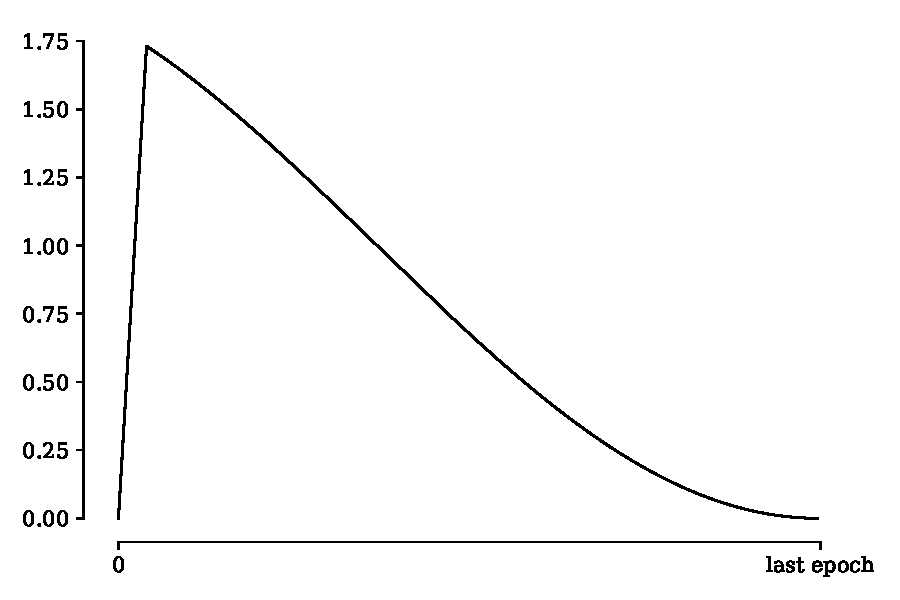
\includegraphics[width=\textwidth]{figs/cosine_annealing_schedule.pdf}
    \caption{Learning rate schedule: a warm-up is performed before the learning rate is adjusted using a cosine annealing schedule. In this example, the learning rate linearly scales to 1.75 before decreasing back to near-zero at the last epoch.}
    \label{fig:cosine_annealing_lr}
\end{marginfigure}

\begin{equation}
    \label{eq:sqrt_lr}
    Learning Rate = 0.075 * \sqrt{Batch Size}
\end{equation}

For linear evaluation, we use the Adam optimiser with a learning rate of $0.0003$ and a weight decay of $10^{-6}$. Backpropagation is only done in the fine-tune head, i.e., it only optimises the linear layer or MLP. The pre-trained encoder remains frozen in all evaluation procedures, for the full classification, efficient classification and transfer learning experiments.
We also employ an early stopping mechanism when the validation scores do not improve for 3 epochs. \footnote{Early stopping stops training on the larger train set, when it has shown to generalise on a smaller validation set.}
\chapter{Experimental Results}\label{sec:results}

\begin{quote}
    In this chapter, we outline the results obtained from the experiments and detail the outcomes of the ablation study. The quality of our models' representations are evaluated using the music classification task.
\end{quote}

\begin{table}
    \centering
    \begin{tabular}{@{}llcc@{}}\toprule
        Model & Dataset & $\text{ROC-AUC}_\text{TAG}$ & $\text{PR-AUC}_\text{TAG}$ \\ \midrule
        % \multicolumn{4}{c}{MTAT-Trained Experiments}\\\addlinespace
        CLMR (ours) & MTAT & 88.49 (\textbf{89.25}) & \textbf{35.37} (\textbf{35.89}) \\
        Pons et al.$^\dagger$ & MTAT & 89.05 & 34.92 \\
        SampleCNN$^\dagger$ & MTAT & 88.56 & 34.38 \\
        CPC (ours) & MTAT & 86.60 (87.99) & 30.98 (33.04) \\
        1D CNN$^\dagger$ & MTAT & 85.58 & 29.59 \\\midrule
        Pons et al.$^\dagger$ & MSD & 87.41 & \textbf{28.53} \\
        SampleCNN$^\dagger$ & MSD & \textbf{88.42} & - \\
        CLMR (ours) & MSD & 85.66 & 24.98 \\
        \bottomrule
    \end{tabular}
    \caption{Tag prediction performance on the MagnaTagATune (MTAT) dataset and Million Song Dataset (MSD), compared with fully supervised models$^\dagger$ trained on raw audio waveforms.
    We omit works that operate on audio in the time-frequency domain.
For the supervised models, the tag-wise scores are obtained by end-to-end training.
For the self-supervised models, the scores are obtained by training a \emph{linear}, logistic regression classifier using the representations from self-supervised pre-training.
Scores in parenthesis show performance when adding one hidden layer to the logistic regression classifier, making it a simple multi-layer perceptron.}
    \label{tab:results}
\end{table}


\section{Quantitative Evaluation}
The most important goal set out in this thesis, is to evaluate the difference in performance between a fully supervised and a self-supervised objective when learning representations, using the exact same encoder set-up. The CLMR model in our experiments uses the SampleCNN encoder network. When SampleCNN is trained in a fully supervised manner, it reaches an PR-AUC score of 34.92. CLMR exceeds this supervised benchmark with a PR-AUC of 35.37, despite task-agnostic, self-supervised pre-training and a \textit{linear} classifier for fine-tuning. An additional 0.5 PR-AUC performance gain is added by adding one extra hidden layer to the classifier. Evaluation scores of the best-performing CLMR, CPC and other wave-form based models are shown in Table \ref{tab:results}.

CLMR also outperforms the current state-of-the-art waveform-based model in the task of automatic music tagging \cite{pons_end--end_2017} in both evaluation metrics for the MagnaTagATune dataset.

The performance on the Million Song Dataset is lower than that of SampleCNN. The highest evaluation scores for the MagnaTagATune dataset are obtained after very long pre-training (10\,000 epochs), of which the details are outlined in Section \ref{sec:additional_experiments}. While this is feasible for a dataset of the size of MagnaTagATune's, we did not have the equipment available to run the experiment for so long on the Million Song Dataset. Additionally, we attribute the difference in performance to the more semantically complex tags in the Million Song Dataset, e.g., `catchy', `sexy', `happy', or more similar tags, e.g., `progressive rock', `clsasic rock' and `indie rock', which may not be linearly separable. 

CPC also shows competitive performance with fully supervised models in the music classification task, despite being pre-trained without ground truth and using a simple, linear classifier for evaluation.
Despite CPC's good performance, self-supervised training indeed does not require a memory bank or more complex loss functions, e.g., those incorporating mutual information or more explicit negative sampling strategies, to learn useful representations.


\section{Qualitative Analysis}
For a qualitative view of the representations, we show how cleanly they are  separable using a $t$-SNE manifold in Figure \ref{fig:tsne_manifold}.
Figure \ref{fig:tag_scores} shows in more detail that the difference in performance between self-supervised and supervised models is marginal: there is no single tag performance difference larger than 4\% ROC-AUC, and for practical purposes, CLMR and CPC retrieve tags practically identically to supervised models.

Figure \ref{fig:tag_scores} also shows that it is especially hard for the self-supervised models to distinguish more semantically complex tags, e.g., `weird', `new age', some instrumental tags, e.g., `stiar', `female/male voice', or the absence of a vocal, i.e., `no vocal'. Similarly to some of the tags in the Million Song Dataset, these may be harder to linearly separate.


\begin{figure}[h]
    \centering
    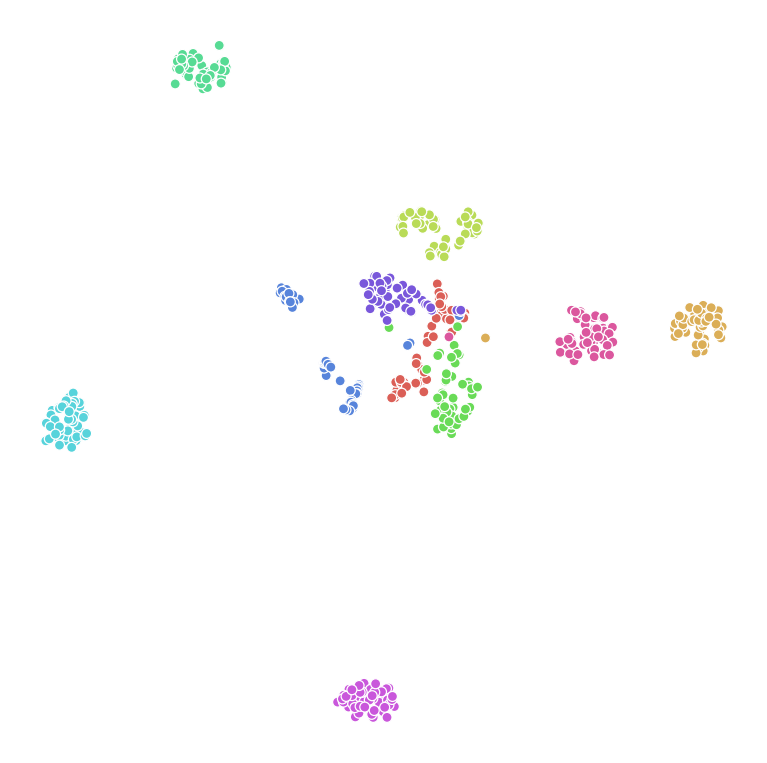
\includegraphics[width=0.9\textwidth]{figs/tsne-clmr.png}
    \caption{$t$-SNE manifold visualisation from audio representations learned by a converged CLMR model of a subset of 10 tracks with each 60 segments.
Every color represents a separate track.}
    \label{fig:tsne_manifold}
\end{figure}

\begin{figure*}[h]
    \centering
    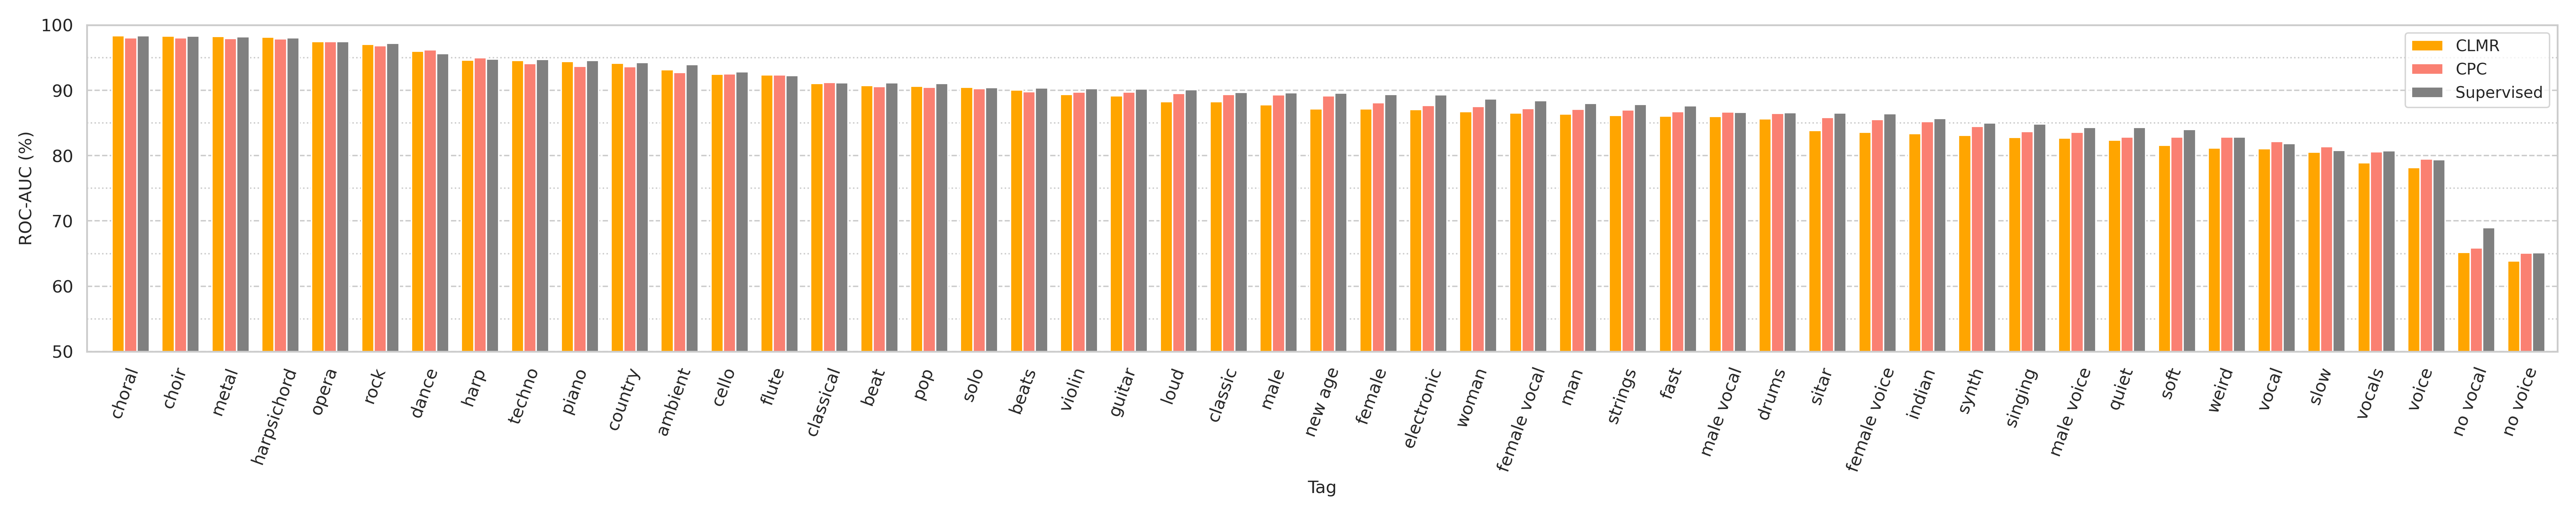
\includegraphics[width=\textwidth]{figs/tag_retrieval.png}
    \caption{Tag-wise ROC-AUC scores for the top-50 tags in the MagnaTagATune dataset, reported for linear, logistic regression classifiers trained on representations of self-supervised models CLMR and CPC, and compared to a fully supervised, end-to-end SampleCNN model.}
    \label{fig:tag_scores}
\end{figure*}


\section{Data Augmentations}\label{sec:data_augmentations}
The CLMR model relies on a pipeline of strong data augmentations to facilitate the learning of representations that are more robust and allow for better generalisation in the downstream task.
In Figure \ref{fig:transformation_study}, we show the PR-AUC linear evaluation score that is achieved when taking a random slice of audio (`random cropping') and performing one additional, individual augmentation.
While all datasets contain songs of variable length, we always sample a random slice of audio of the same size before applying other augmentations.
Since we always have to take a random slice, it makes it harder to assess the individual contribution of each augmentation to the downstream task performance.
We therefore consider an asymmetric data transformation setting: we only apply the augmentation pipeline to one branch of the framework, while we settle with an identity function for the other branch (i.e., $t(x_j) = x_j$) \cite{chen_simple_2020}. The transformations on the augmentation branch are applied with probability $p_t=1$, i.e., the transformation is always applied.

When only taking a random slice of audio (i.e., a `crop'), we achieve a PR-AUC score of 30.5.
Most augmentations show a similar increase in performance of ±31.5, while adding gain or delay does not impact performance as much.
Adding a filter to the pipeline increases the downstream performance significantly.

\begin{figure*}[h]
    \centering
    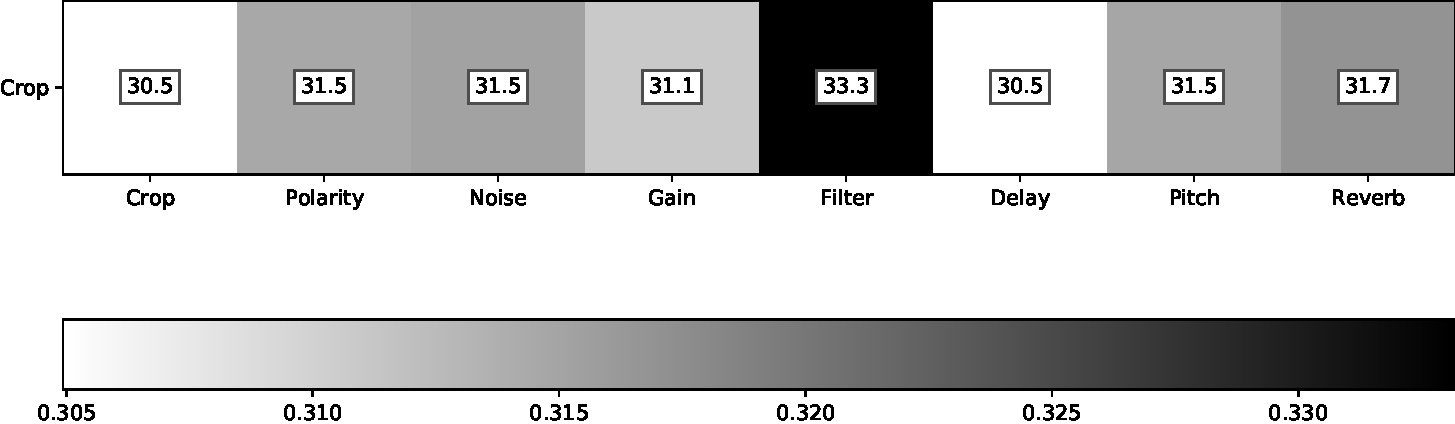
\includegraphics[width=\columnwidth]{figs/transformation_study.pdf}
    \caption{The achieved $\mathrm{PR-AUC}_{\mathrm{TAG}}$ score using a random crop together with one other transformation}
    \label{fig:transformation_study}
\end{figure*}

Besides evaluating the individual contribution of each augmentation with a probability of $p_t = 1$, we also vary this probability: $p_t \in \{ 0, 0.4, 0.8 \}$.
This is done to assess the optimal amount of augmentation to each example, i.e., the contrastive learning task should not be too hard, neither too simple, for learning effective representations in the downstream music classification task.
The linear evaluation PR-AUC score is shown for each augmentation under a different probability $p_t$ in Figure \ref{fig:transformation_probabilities}. For the Polarity and Filter transformations, performing them more often with a probability of $p_t = 0.8$ is beneficial. For the Delay, Pitch and Reverb transformations, a transformation probability of $p_t = 0.4$ works better than performing them more aggressively.

\begin{figure}[h]
    \centering
    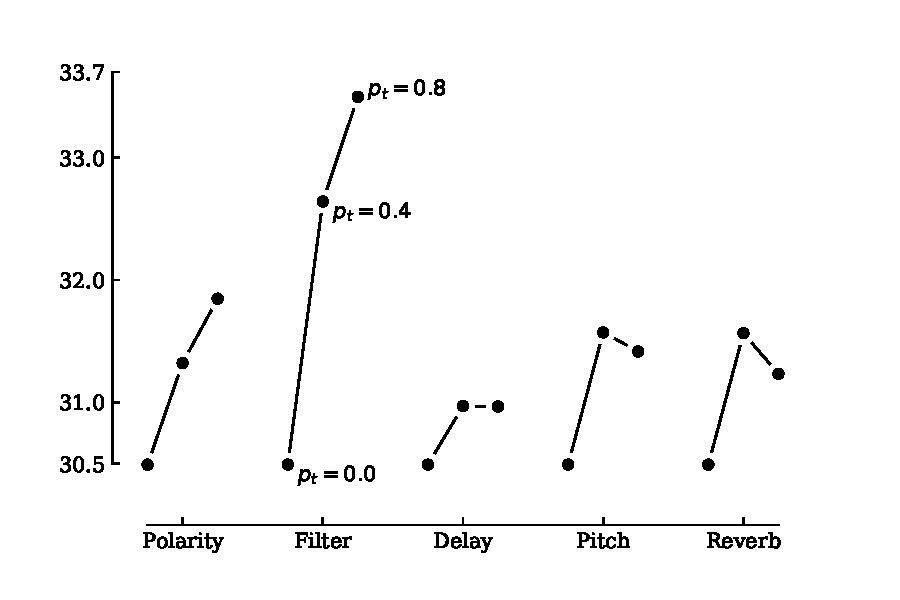
\includegraphics[width=\columnwidth]{figs/transformation_probabilities.pdf}
    \caption[-5cm]{$\mathrm{PR-AUC}_{\mathrm{TAG}}$ scores for transformations under different, consecutive probabilities $p \in \{ 0.0, 0.4, 0.8 \}$}
    \label{fig:transformation_probabilities}
\end{figure}


\section{Efficient Classification Experiments}
When training on a specific task like music classification, only a limited amount of labeled data may be available. To test the efficient classification capability of the CLMR model, we fine-tune the linear classifier on 1\% of the labels in the dataset and report its performance. During the task-agnostic, self-supervised pre-training phase, 100\% of the data is used. As outlined previously, the representations that are learned during this phase are subsequently used during linear evaluation.

Figure \ref{fig:perc_train_data_magnatagatune} and \ref{fig:perc_train_data_msd} show the PR-AUC scores obtained when increasing the amount of labels available during fine-tuning.
For both datasets, fine-tuning using just $1\%$ of the labels yields a large performance difference compared to training in a fully supervised manner, while using the same amount of labels.

\begin{figure}[h]
    \centering
    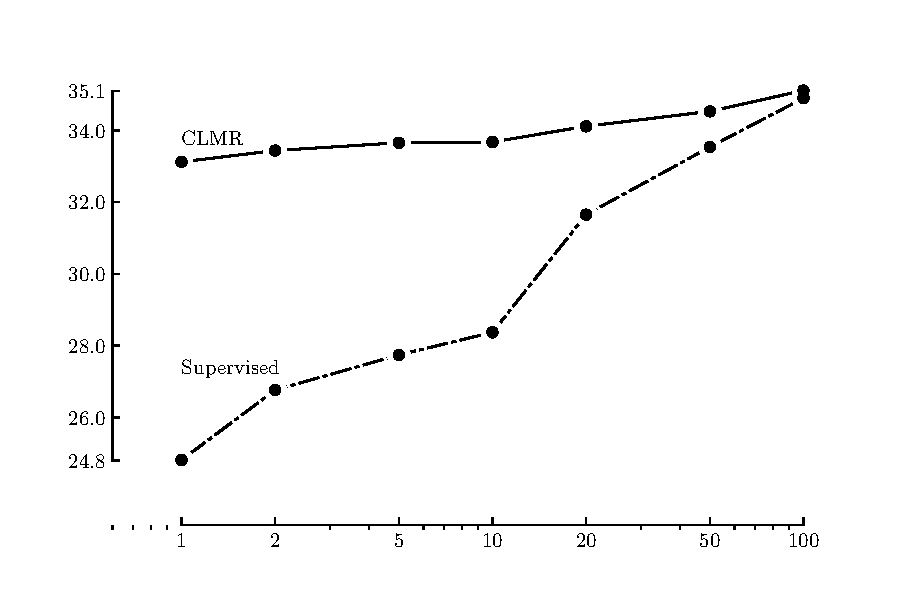
\includegraphics[width=\columnwidth]{figs/perc_train_data_magnatagatune.pdf}
    \caption{Percentage of labels used for training vs. the achieved $\mathrm{PR-AUC}_{\mathrm{TAG}}$ score on the MagnaTagATune dataset}
    \label{fig:perc_train_data_magnatagatune}
\end{figure}


Using 100$\times$ fewer labels, CLMR scores 33.1\% PR-AUC compared to 24.8\% PR-AUC obtained with an equivalent, end-to-end trained supervised model.
Pre-training using a self-supervised objective without labels therefore substantially improves efficient classification: only $1\%$ of the labels are required while maintaining a similar performance.

For the Million Song Dataset, a fully supervised end-to-end trained model exceeds CLMR at $10\%$ of the labels, which are 24,190 unique songs in total. Beyond this amount of music, CLMR is unable to perform in a trend similar to the supervised model.

\begin{figure}[h]
    \centering
    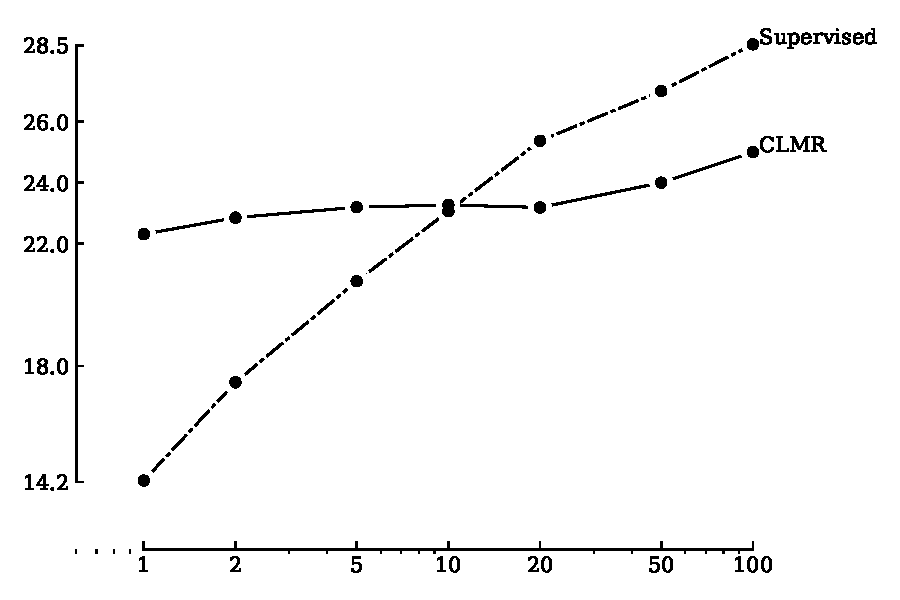
\includegraphics[width=\columnwidth]{figs/perc_train_data_msd.pdf}
    \caption{Percentage of labels used for training vs. the achieved $\mathrm{PR-AUC}_{\mathrm{TAG}}$ score on the Million Song Dataset.}
    \label{fig:perc_train_data_msd}
\end{figure}



\section{Transfer Learning Experiments}
The results of the transfer learning experiments are shown in Table \ref{tab:magnatagatune_results}.
Both CPC and CLMR show the ability to learn effective representations from datasets different from the evaluation dataset without ground truth, and even exceed accuracy scores of previous, supervised end-to-end systems on raw audio \cite{dieleman2014end}.
Moreover, both models demonstrate the ability to learn useful representations on the much smaller GTZAN and Billboard datasets.
The CLMR model performs better when it is pre-trained on larger datasets, which is expected as it heavily relies on the number of unique, independent examples that make the contrastive learning task harder, resulting in more robust representations.
When pre-training on smaller datasets, the autoregressive modelling in CPC can find more useful representations for downstream tasks.
%contribute to more useful representations for downstream tasks.

\begin{table}[h]
    \centering
    \begin{tabular}{@{}lllcc@{}}\toprule
        Model & Train Dataset & Eval.
        Dataset &  ROC-AUC & PR-AUC \\ \midrule
        CLMR & MSD & MTAT &  86.57 & 32.04 \\
        CPC & FMA & MTAT & 86.34 (87.79) & 30.71 (32.47) \\
        CLMR & FMA & MTAT & 86.22 (86.63) & 30.58 (31.22) \\
        CPC & Billboard & MTAT & 85.78 (86.25) & 29.68 (30.15) \\
        CPC & GTZAN & MTAT & 83.44 (86.06) & 26.88 (29.72) \\
        CLMR & Billboard & MTAT & 82.73 (84.22) & 26.86 (27.82) \\
        CLMR & GTZAN & MTAT & 81.88 (85.43) & 26.18 (29.49) \\
        \bottomrule
    \end{tabular}
    \caption{Performance of the self-supervised models when pre-trained on datasets different from the evaluation dataset, again using a linear classifier to evaluate.}
    \label{tab:magnatagatune_results}
\end{table}

\newpage

\section{Additional Experiments}\label{sec:additional_experiments}
\subsection{Mini-batch Size}\label{sec:exp_mini_batch_size}
The complexity of the pretext task increases with larger mini-batch sizes. To reiterate: in our pretext task, it is harder for the the model to infer the positive pair when increasing the pool of negative examples.
To further study the quality of the repesentations for the downstream task performance, given the increase of complexity of the pretext task, we experimented with varying mini-batch sizes while keeping all other parameters the same.

We use the default sample rate of 22\,050~Hz, the $3^9$ SampleCNN encoder network, train all experiments for 3\,000 epochs and set the transformation probabilities to their optimal value, as demonstrated in Section \ref{sec:data_augmentations}. All models with varying mini-batch sizes are trained from scratch and evaluated using the linear evaluation procudure outlined in Section \ref{sec:evaluation}.

While our smallest model already shows competitive performance compared to fully supervised models, the performance increased when using 96 examples per mini-batch. Our largest model did not perform as expected, and scores consistently lower than our middle-sized model. This may be attributed to a sub-optimal configuration of the optimiser, i.e., the LARS optimiser that is used for larger mini-batch sizes. Another theory, is that the task of inferring the positive pair of 2.6 second long audio fragments, in a pool of 912 negative samples, may require even longer training, or is simply too hard. The results of this experiment are shown in Table \ref{tab:mini_batch_ablation}.


\begin{table*}
    \centering
    \begin{tabular}{lllll}\toprule
    Mini-batch Size & $\text{ROC-AUC}_{\text{TAG}}$ & $\text{PR-AUC}_{\text{TAG}}$ & $\text{ROC-AUC}_{\text{CLIP}}$ & $\text{PR-AUC}_{\text{CLIP}}$ \\\midrule
    456 & 88.13 & 34.87 & 92.96 & 68.90 \\
    96 & 88.49 & 35.11 & 93.07 & 69.20 \\
    48 & 87.91 & 34.56 & 92.88 & 68.75 \\\bottomrule
    \end{tabular}
    \caption[][24pt]{Effect of the mini-batch size used during self-supervised training on the music classification task performance.}
    \label{tab:mini_batch_ablation}
\end{table*}

\newpage

\subsection{Training Duration}
Contrastive learning techniques have shown to benefit from longer training compared to their supervised equivalent \cite{chen_simple_2020}. While larger mini-batch sizes increase the number of negative examples the model can `see' simultaneously, training for a longer time increases the number of negative examples the model sees overall. We vary the number of epochs we train the model for, while we keep all other parameters constant, i.e., identically to those described in Section \ref{sec:exp_mini_batch_size}. The mini-batch size is set to 96 and all models are again trained from scratch and evaluated using the linear evaluation procedure.

Increasing the self-supervised training duration improves the downstream task performance. Our best results are obtained when training the CLMR model for 10\,000 epochs. When training the logistic, linear regression classifier on the learned representations, it perfroms better than a fully, end-to-end trained supervised model. The results of this experiment are shown in Table \ref{tab:epoch_ablation}.


\begin{table*}
    \centering
    \begin{tabular}{lllll}\toprule
    Epochs & $\text{ROC-AUC}_{\text{TAG}}$ & $\text{PR-AUC}_{\text{TAG}}$ & $\text{ROC-AUC}_{\text{CLIP}}$ & $\text{PR-AUC}_{\text{CLIP}}$ \\\midrule
    10\,000 & 88.47 (89.25) & 35.37 (35.89) & 93.16 (93.48) & 69.32 (70.03) \\
    3\,000 & 88.49 (88.94) & 35.11 (35.46) & 93.07 (93.27) & 69.20 (69.74) \\
    1\,000 & 88.31 (88.64) & 34.40 (34.86) & 92.89 (93.08) & 68.59 (69.15) \\\bottomrule
    \end{tabular}
    \caption[][24pt]{Effect of the self-supervised training duration on the music classification task performance.}
    \label{tab:epoch_ablation}
\end{table*}




\subsection{Sample Rates}    
When re-sampling the audio to 8\,000~Hz and 16\,000~Hz respectively, there is a marginal penalty to the final scores for the self-supervised models, which is in line with previous work \cite{lee2018samplecnn}. In Table \ref{tab:sample_rate_ablation}, we show all linear evaluation scores when no additional transformations are performed (i.e., only random cropping) to isolate the contribution of each individual sample rate.


\begin{table*}
    \centering
        \begin{tabular}{lllll}\toprule
        Sample rate & $\text{ROC-AUC}_{\text{TAG}}$ & $\text{PR-AUC}_{\text{TAG}}$ & $\text{ROC-AUC}_{\text{CLIP}}$ & $\text{PR-AUC}_{\text{CLIP}}$ \\\midrule
        8\,000 & 84.78 & 29.77 & 90.60 & 62.94 \\
        16\,000 & 85.46 & 30.42 & 90.97 & 64.08 \\
        22\,050 & 85.82 & 30.49 & 91.25 & 64.78 \\                       
        \bottomrule
        \end{tabular}
    \caption[][24pt]{Effect of the sample rate on tag prediction performance.}
    \label{tab:sample_rate_ablation}
\end{table*}


\subsection{Temperature}
The temperature parameter $\tau$ in the NT-Xent loss function (Equation \ref{eq:loss_function}) controls the penalty given to the negative samples. The experiments in Table \ref{tab:temperature_ablation} are run using a mini-batch size of 96, which is a smaller mini-batch size than those used in the original SimCLR paper (i.e., $\leq 4096$ samples per mini-batch) \cite{chen_simple_2020}. Consequently, the performance difference is marginal. Again, no additional transformations except random cropping are applied in this experiment to isolate the contribution of this temperature parameter.

\begin{table*}
    \centering
    \begin{tabular}{lllll}\toprule
    Temperature & $\text{ROC-AUC}_{\text{TAG}}$ & $\text{PR-AUC}_{\text{TAG}}$ & $\text{ROC-AUC}_{\text{CLIP}}$ & $\text{PR-AUC}_{\text{CLIP}}$ \\\midrule
    0.1  & 85.82  & 30.33 & 91.18 & 64.10 \\
    0.3 & 85.58 & 30.35 & 91.21  & 64.38 \\
    0.5 & 85.82 & 30.49 & 91.25 & 64.78 \\                       
    \bottomrule
    \end{tabular}
    \caption[][24pt]{Ablation study of the temperature parameter in the NT-Xent loss function.}
    \label{tab:temperature_ablation}
\end{table*}


\section*{Summary}
In this chapter, we presented the results of this thesis. We showed that CLMR learns effective representations from raw signals of musical audio. Despite self-supervised pre-training and fine-tuning a linear classifier on the representations, we achieve strong performance on the downstream music classification task. CLMR outperforms the current state-of-the-art waveform-based model on the MagnaTagATune dataset, but it requires longer training to show comparable results on the Million Song Dataset.

We studied the contribution of seven different data augmentations, of which five were studied with altering transformation probabilities, to the robustness of the learned representations. In line with previous research on self-supervised learning, we demonstrated that strong data augmentations during pre-training benefit the downstream task performance. We also showed that too strong augmentations can negatively impact the usability of the representations.

It is common in MIR to have limited labeled data available for training a neural network. Therefore, we tested the efficient classification capability of the CLMR model. We fine-tuned the linear classifier on only 1\% of the labels in the dataset, using representations learned during the self-supervised pre-training phase on 100\% of the data. The linear classifier still achieved 33.1\% PR-AUC, compared to 24.8\% PR-AUC with a fully supervised end-to-end model, despite using 100$\times$ fewer labels.

Lastly, we showed that the learned representations are transferable across different musical corpora. When pre-training CLMR on a large, out-of-domain music dataset, and linearly evaluating the representations on another music dataset, the cost is a relatively small performance margin.
\chapter{Interpretability}

\begin{quote}
    In this chapter, we describe the experiments that were used to qualitatively analyse the features learned by the CLMR model, and get a deeper understanding of the model's learned representations. First, we visualise the filters of the convolutional layers to show what frequencies each filter is most sensitive to. Subsequently, we introduce a factor analysis that guides our qualitative analysis of every dimension in the fine-tuned head (linear layer or MLP). Lastly, we employ a recently published source separation technique to reconstruct the audio that the network is most confident of when predicting targets.
\end{quote}

The following sections describe the experiments that were performed on the frozen, pre-trained feature extractor network \footnote{In our case, the SampleCNN encoder} in the CLMR framework. In other words, the representations analysed in this chapter are those that were learned in a task-agnostic, self-supervised manner, not those that were learned after the fine-tuning phase.

\section{Visualising Filters}
Figure \ref{fig:filter_visualisation} shows the magnitude spectrum of the learned filters of the sample-level convolutional layers (layers 1, 4 and 6) for CLMR and CPC, pre-trained on the MagnaTagATune and Billboard dataset.
In CLMR, the first layer is sensitive to a single, very small band of frequencies around 7500~Hz, while in higher layers, the filters spread themselves first linearly and then non-linearly across the full range.
CPC shows a similar pattern in the lowest layer, but shows a strong activation of two frequencies that span an octave.
Interestingly, CLMR pre-trained on the Billboard dataset shows a similar filter structure to fully supervised models that were trained on the MagnaTagATune dataset \cite{dieleman2014end,lee2018samplecnn}. For comparison, these are shown in Figure \ref{fig:samplecnn_filters}.
The Billboard dataset is significantly less diverse in genre, suggesting the self-supervised model focuses more on such frequency-band related differences than it does for the more genre-diverse MagnaTagATune.


\begin{figure}
    \centering
    \subcaptionbox{CLMR$^{(1)}_{\mathrm{MTAT}}$\label{fig:1a}}{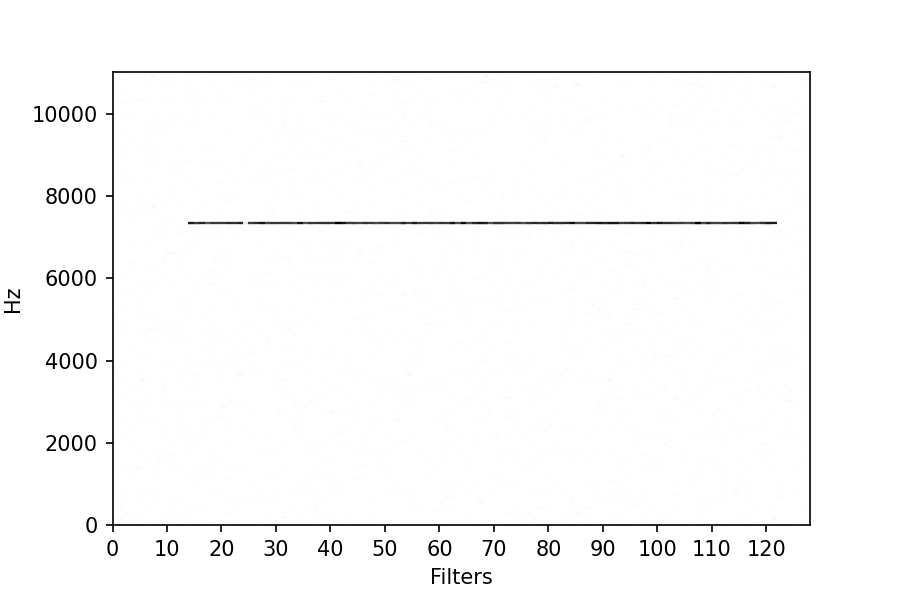
\includegraphics[width=.33\textwidth]{figs/magnatagatune/clmr_spectrum/epoch1490_layer0.png}}\hfill
    \subcaptionbox{CLMR$^{(4)}_{\mathrm{MTAT}}$\label{fig:1a}}{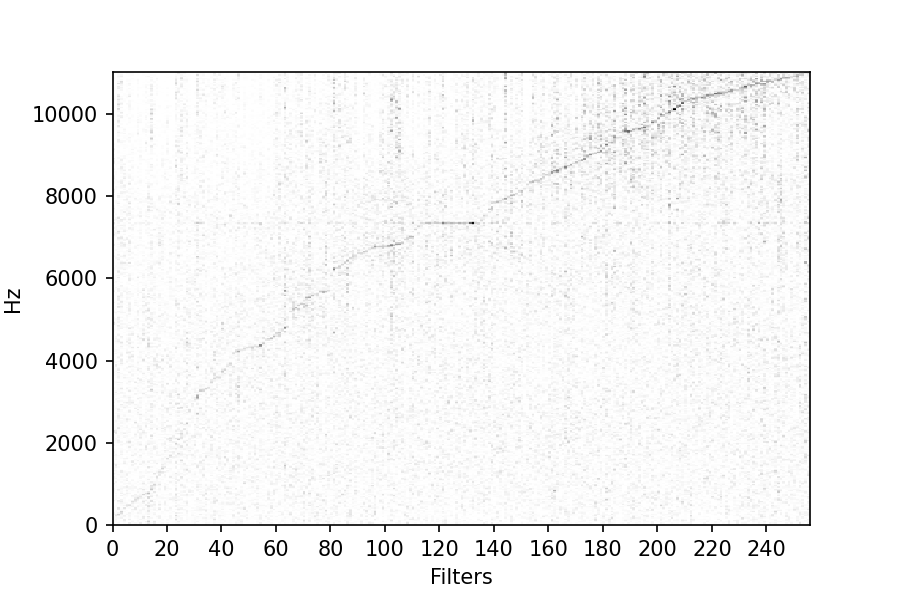
\includegraphics[width=.33\textwidth]{figs/magnatagatune/clmr_spectrum/epoch1490_layer3.png}}\hfill
    \subcaptionbox{CLMR$^{(6)}_{\mathrm{MTAT}}$\label{fig:1a}}{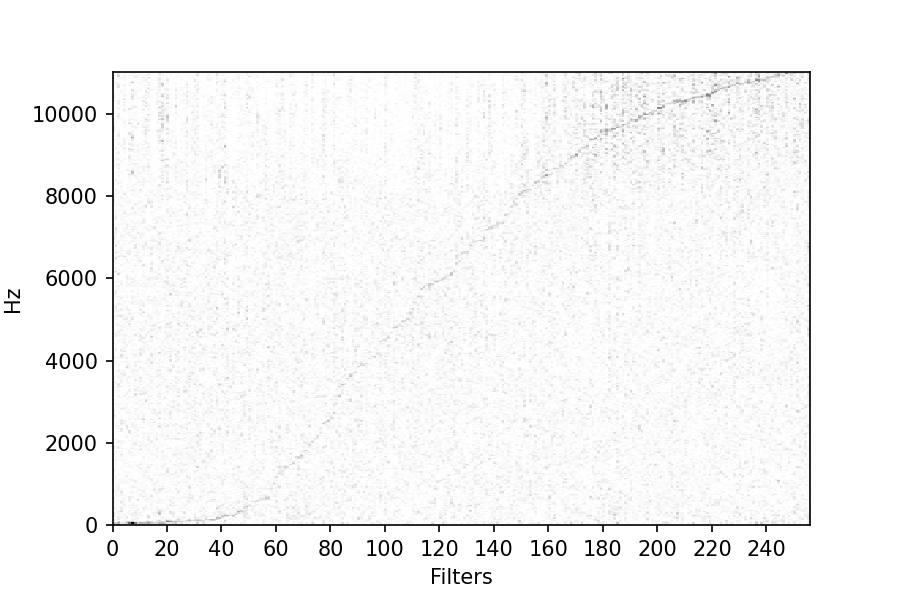
\includegraphics[width=.33\textwidth]{figs/magnatagatune/clmr_spectrum/epoch1490_layer5.png}}

    \subcaptionbox{CPC$^{(1)}_{\mathrm{MTAT}}$\label{fig:1a}}{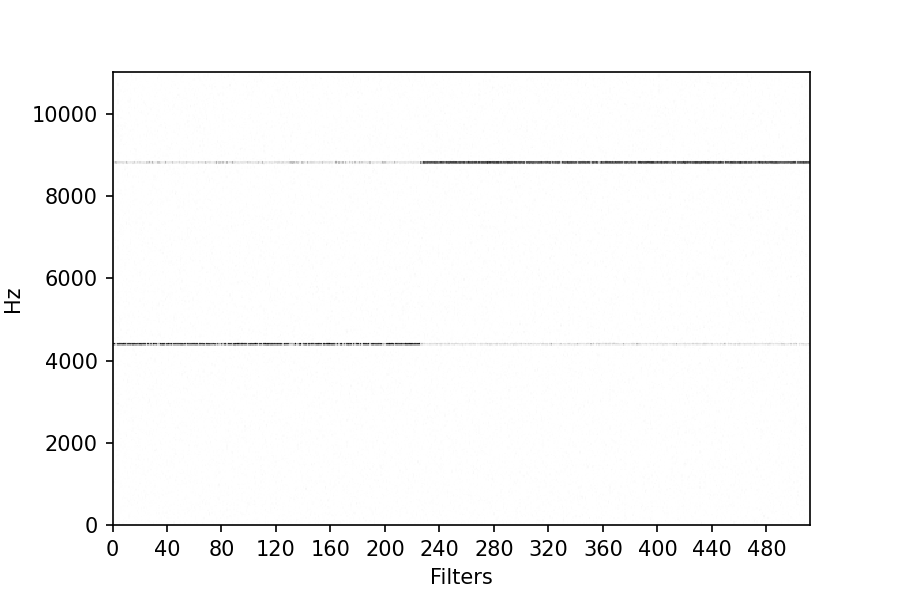
\includegraphics[width=.33\textwidth]{figs/magnatagatune/cpc_spectrum/epoch670_layer0.png}}\hfill
    \subcaptionbox{CPC$^{(4)}_{\mathrm{MTAT}}$\label{fig:1a}}{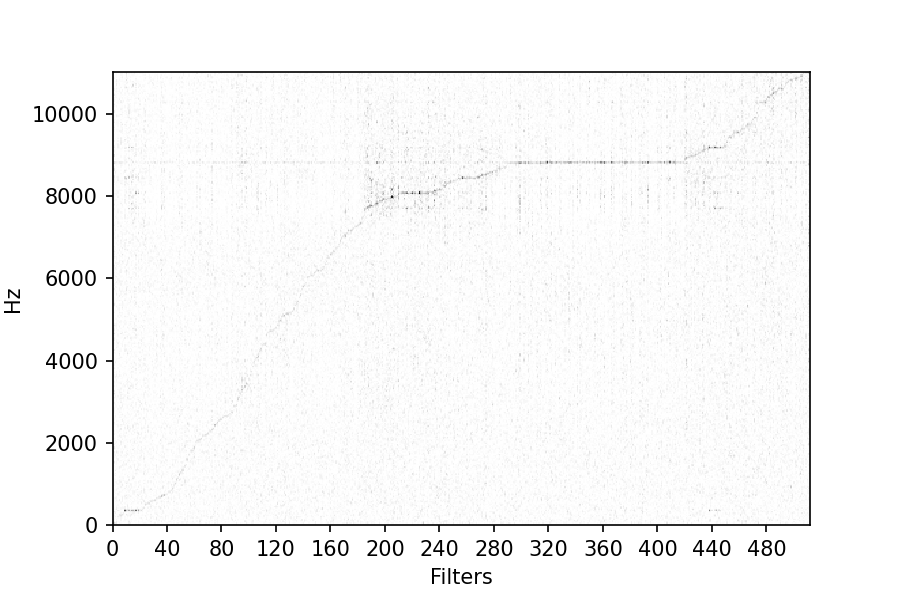
\includegraphics[width=.33\textwidth]{figs/magnatagatune/cpc_spectrum/epoch670_layer3.png}}\hfill
    \subcaptionbox{CPC$^{(6)}_{\mathrm{MTAT}}$\label{fig:1a}}{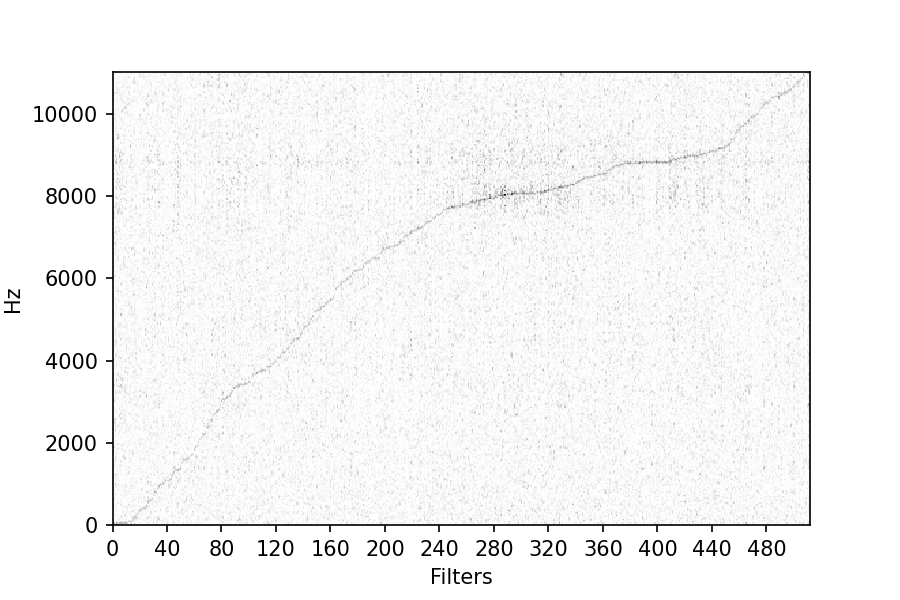
\includegraphics[width=.33\textwidth]{figs/magnatagatune/cpc_spectrum/epoch670_layer5.png}}

    \caption[][-3cm]{Normalised magnitude spectrum of the filters of the self-supervised models in the sample-level convolution layers, sorted by the frequency of the peak magnitude. Gradient ascent is performed on a randomly initialised waveform of 729 samples (close to typical frame size) and its magnitude spectrum is calculated subsequently. Each vertical line in the graph represents the frequency spectrum of a different filter. The first three images are taken from a pre-trained, converged CLMR model, the last three from a CPC model. Both are trained on the MagnaTagATune dataset.}
    \label{fig:filter_visualisation}
\end{figure}

\begin{figure}
    \centering
    \subcaptionbox{CLMR$^{(1)}_{\mathrm{Billboard}}$\label{fig:1a}}{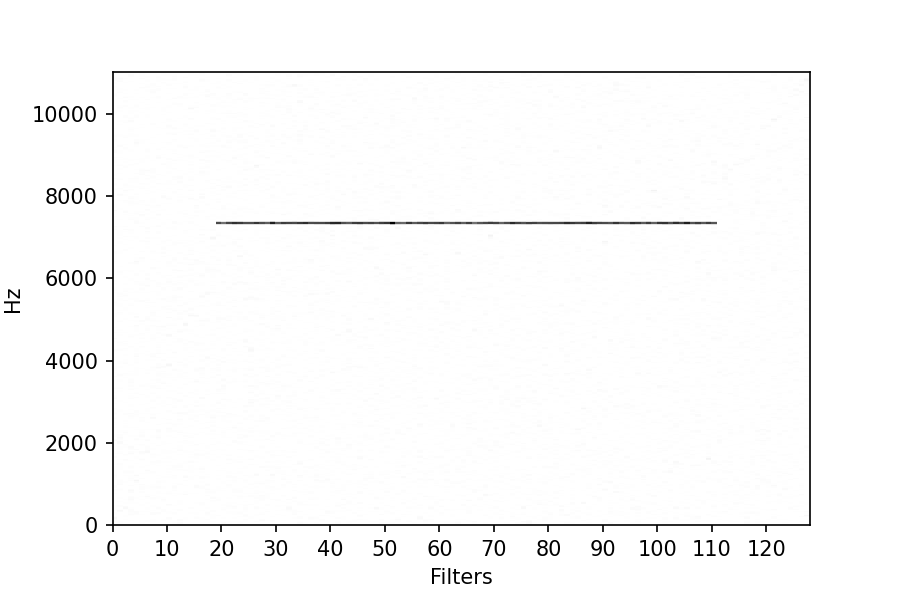
\includegraphics[width=.33\textwidth]{figs/billboard/clmr_spectrum/epoch1490_layer0.png}}\hfill
    \subcaptionbox{CLMR$^{(4)}_{\mathrm{Billboard}}$\label{fig:1a}}{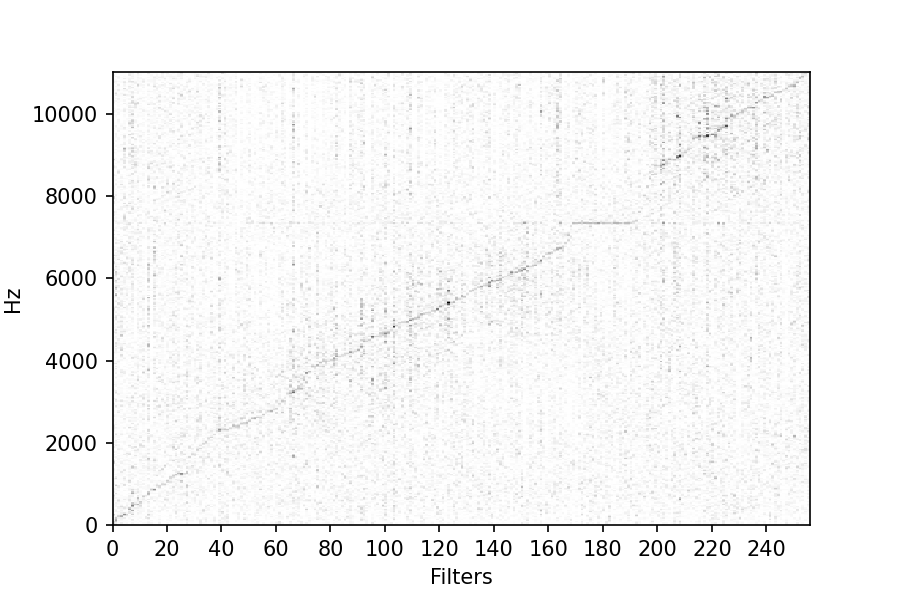
\includegraphics[width=.33\textwidth]{figs/billboard/clmr_spectrum/epoch1490_layer3.png}}\hfill
    \subcaptionbox{CLMR$^{(6)}_{\mathrm{Billboard}}$\label{fig:1a}}{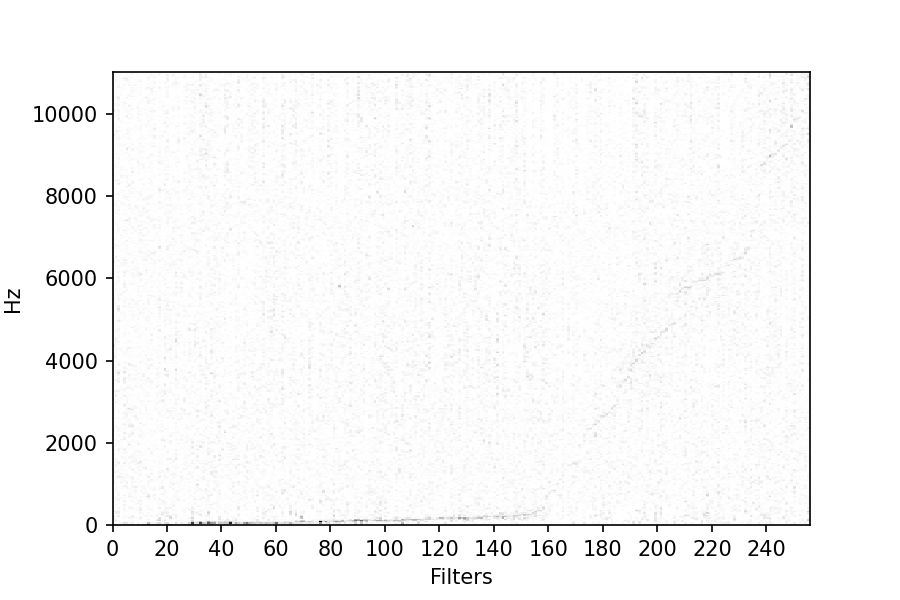
\includegraphics[width=.33\textwidth]{figs/billboard/clmr_spectrum/epoch1490_layer5.png}}

    \subcaptionbox{CPC$^{(1)}_{\mathrm{Billboard}}$\label{fig:1a}}{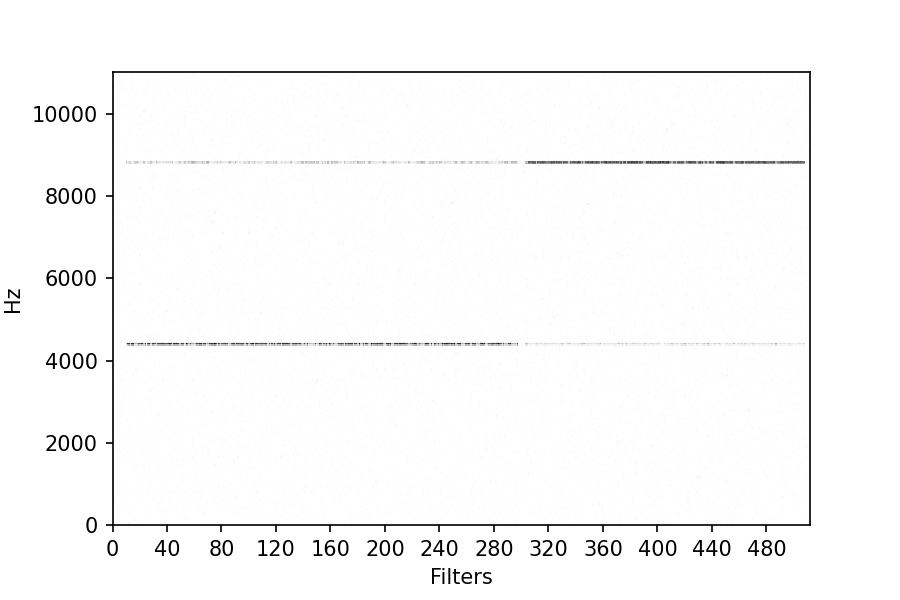
\includegraphics[width=.33\textwidth]{figs/billboard/cpc_spectrum/epoch1490_layer0.png}}\hfill
    \subcaptionbox{CPC$^{(4)}_{\mathrm{Billboard}}$\label{fig:1a}}{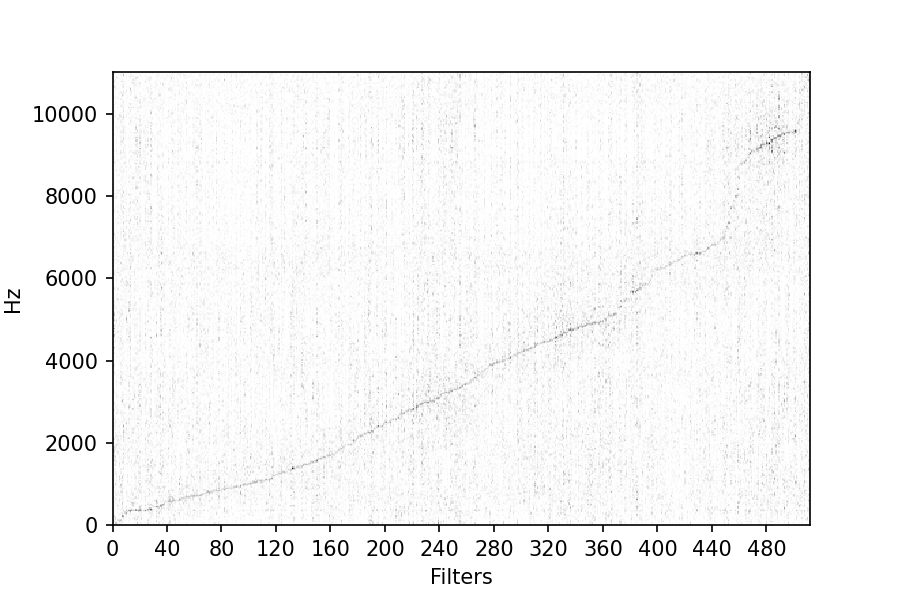
\includegraphics[width=.33\textwidth]{figs/billboard/cpc_spectrum/epoch1490_layer3.png}}\hfill
    \subcaptionbox{CPC$^{(6)}_{\mathrm{Billboard}}$\label{fig:1a}}{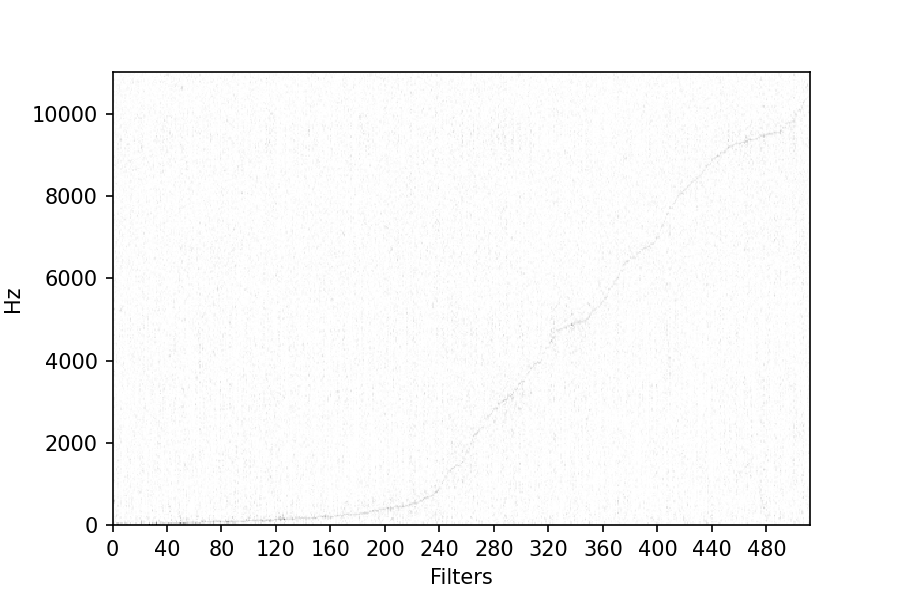
\includegraphics[width=.33\textwidth]{figs/billboard/cpc_spectrum/epoch1490_layer5.png}}
    \caption{Normalised magnitude spectra, generated using the method described in Figure \ref{fig:filter_visualisation}. These CLMR and CPC models were trained on the Billboard dataset}
    \label{fig:filter_visualisation_billboard}
\end{figure}

\begin{figure}
    \centering
    \includegraphics[width=\textwidth]{figs/samplecnn_filters.png}
    \caption{Normalised magnitude spectrum of filters from layers 1 - 6 of a fully end-to-end trained supervised SampleCNN network. Figure is taken from Figure 3 in \cite{lee2018samplecnn}.}
    \label{fig:samplecnn_filters}
\end{figure}


\section{Activations}
\label{sec:activations}
Figure \ref{fig:magnatagatune_activations} and \ref{fig:msd_activations} show the mean activations\footnote{We use the term "activations" to describe the values that are obtained from the last convolutional layer of the SampleCNN encoder, i.e., from the 512 filters, when predicting a segment of musical audio.} of the last convolutional block of the SampleCNN encoder for every music segment in the test set, for both the MagnaTagATune and Million Song Dataset respectively. In contrast to the MagnaTagATune activations, the last layer of the encoder from the Million Song Dataset activates more broadly for every track, indicating that the encoder responds more flatly. It is important to note that the feature numbers on the x-axis in Figures \ref{fig:magnatagatune_activations} and \ref{fig:msd_activations} do not correspond to the actual mean activation value - they show how many features were used in the last layer of the SampleCNN encoder. In the following paragraph, we describe a qualitative analysis that uses these activations.

\begin{marginfigure}
    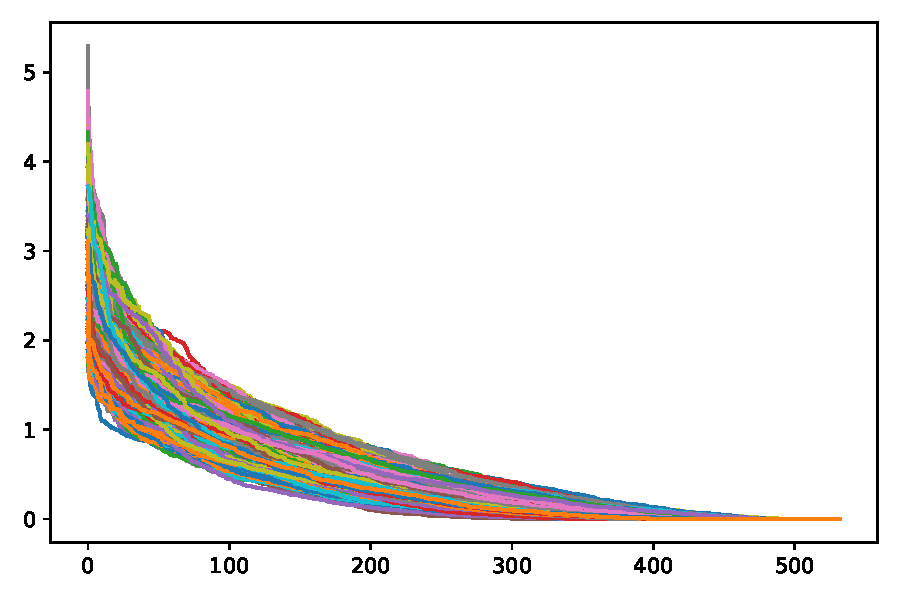
\includegraphics[width=\textwidth]{figs/activations.pdf}
    \caption{Mean activations of 512 features for every music segment, sorted by activation value. Extracted from the encoder of a converged CLMR model trained on the MagnaTagATune dataset.}
    \label{fig:magnatagatune_activations}
\end{marginfigure}

\begin{marginfigure}
    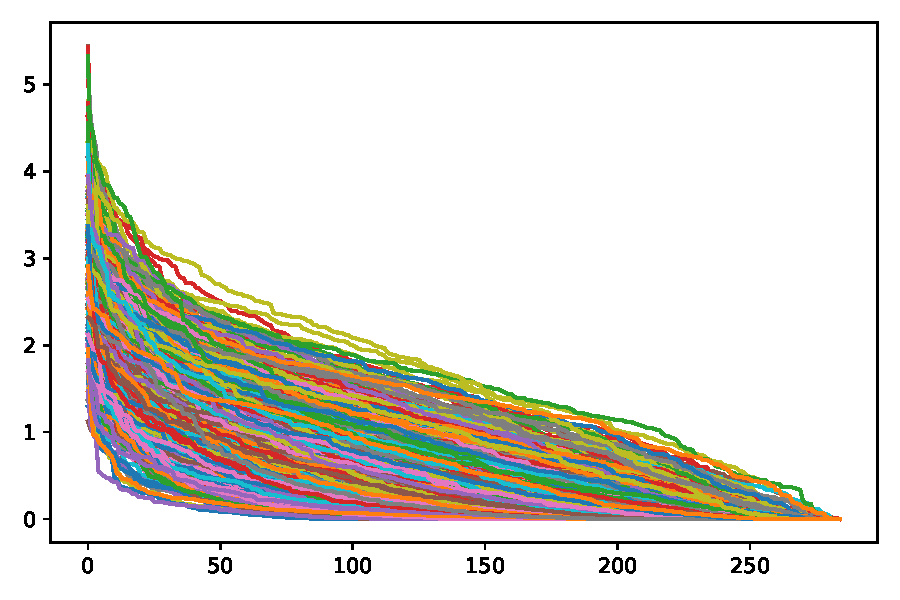
\includegraphics[width=\textwidth]{figs/activations_msd.pdf}
    \caption{Mean activations of 512 features for every music segment, sorted by activation value. Extracted from the encoder of a converged CLMR model trained on the Million Song Dataset.}
    \label{fig:msd_activations}
\end{marginfigure}

\section{Listening Experiment}
We have devised an interface which makes it easy to listen to music segments that were run through the CLMR model.
For any one of the 512 filters (i.e., features) in the last layer of the pre-trained SampleCNN encoder, we calculate the activations for each music segment.
This yields a table of 512 columns of features and $X$ sorted rows based on the activation value of filter.
\footnote{$X$ being the number of data points in the dataset's test set.}

We take the following, basic approach to qualitatively analyse the features learned by our self-supervised model:
\begin{itemize}
    \item We calculate the filter activations of the last convolution layer for all music segments in the test set, yielding a 512-dimensional feature vector for every segment.
    \item We plot these values in a sortable table and including the corresponding, listenable music segment.
    \item We choose a single feature from any of the 512 available, and sort the activation values in a descending order.
    \item We listen to the top-$N$ segments, and write down the sound qualities of those in the upper level (i.e., the first $N$).
\end{itemize}

A screenshot of the listening experiment interface is shown in Figure \ref{fig:listening_experiment}. We guided our listening experiment with factor analysis first. While this did not yield good results, we later used a manual approach described in paragraph \ref{sec:manual_interpretations}. We included the factor analysis paragraph for future improvement.

\section{Factor Analysis}
The following analysis is performed using a converged CLMR model that was pre-trained on the MagnaTagATune dataset.

A factor analysis is used to describe correlated variables using a lower number of unobserved variables, i.e., whether variations of many variables reflect those of fewer variables. To guide our listening experiment, we use varimax rotation on the fully connected 512-dimensional layer that is extracted from the linear (or MLP) head after fine-tuning has converged. We choose to use 3 components and subsequently sort each of the 512-dimensional feature vectors by their factor value per component. These are shown in Figure \ref{fig:varimax_rotation}. This gives us an indication which feature numbers are more closely related.

\begin{figure}[h]
    \centering
    \begin{subfigure}[b]{0.3\textwidth}
        \centering
        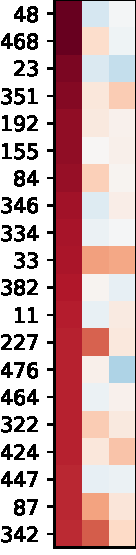
\includegraphics[width=\textwidth]{figs/varimax-magnatagatune-0.pdf}
        \caption{Component 1}
    \end{subfigure}
    \hfill
    \begin{subfigure}[b]{0.3\textwidth}
        \centering
        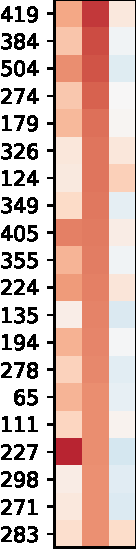
\includegraphics[width=\textwidth]{figs/varimax-magnatagatune-1.pdf}
        \caption{Component 2}
    \end{subfigure}
    \hfill
    \begin{subfigure}[b]{0.3\textwidth}
        \centering
        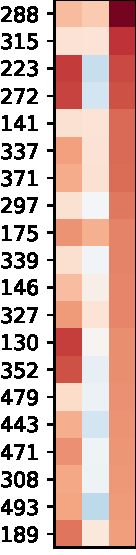
\includegraphics[width=\textwidth]{figs/varimax-magnatagatune-2.pdf}
        \caption{Component 3}
    \end{subfigure}
    \caption[][24pt]{Varimax rotation of 3 components on 512 factors (features) on a pre-trained CLMR model on the MagnaTagATune dataset. The figure shows the 20 strongest factors per component.}
    \label{fig:varimax_rotation}
\end{figure}

After listening to segments that highly activate among the relating features obtained from sorting the factors for each component using varimax, we quickly found that it was biased toward grouping loud, techno/(hard-)rock music together for every single component (i.e., for components 1 - 3). To analyse a possible reason for this behavior, we plotted the number of tags in the top-10 activating segments for every feature number in the 512-dimensional feature vector. This is shown in Figure \ref{fig:tag_frequency}. It shows the more dominantly present tags that are predicted for every feature number, e.g., `techno, `rock', `beat', `loud', `dance'. Most features respond highly to these tags, while other tags like `vocal' or `flute' occur less often. These results do not simply translate to the overall tag frequency: the `guitar' and `classical' tags occur more in the dataset, but show less activations overall than `techno' or `rock'.

While the Factor Analysis grouped together a single, dominant spectral feature, i.e., loudness, and while time is a constraint on the extensivity of this qualitative analysis, we resorted to an easier, but manual intepretation method using \textit{out-of-domain} data.


\section{Out-of-domain Generalisation}\label{sec:manual_interpretations}
To evaluate whether certain features respond to similar spectral qualities, we process both the MagnaTagATune dataset, which the model was pre-trained on, and the Million Song Dataset through the encoder network. In this way, we are able to determine the \textit{out-of-domain generalisation} of the self-supervised model, i.e., is it able to learn features that describe similar sonic qualities of music originating from an entirely different library of music. We extract a 512-dimensional feature vector from the last SampleCNN filters for every segment (as described in Section \ref{sec:activations}), and evaluate whether the same filters respond to the same sonic qualities present in the music segments.

For example, we evaluate whether filter number $412$ highly activates on segments of slow-paced jazz music from both the MagnaTagATune and Million Song Dataset, or not. We describe each feature using sound qualities, e.g., in terms of the frequency spectrum, loudness, and ADSR qualities.\footnote{The attack, decay, sustain, release of the sound.} The filter numbers are pickled by manually listening to the most activating segments of the chosen filter and, when those musical pieces are sufficiently coherent, we listen to the most activating out-of-domain segments of the same filter.

\subsection*{Filter \#51}
\paragraph{MagnaTagATune}
Slow, vocal, string and flute instruments, accompanied by either harpsichord or guitar.
\paragraph{Million Song Dataset}
Slow, vocal accompanied by guitar. Some segments are up-paced jazz, but those recordings contain a lot of noise.

\subsection*{Filter \#61}
\paragraph{MagnaTagATune}
Loud, distorted guitars, vocals, heavy beat, snappy percussion and bass
\paragraph{Million Song Dataset}
Loud, heavy distorted guitars, hip-hop rapping vocals, percussive bass.

\subsection*{Filter \#76}
\paragraph{MagnaTagATune}
Slow string music, vocal, classical, and solo flute, slow attack, not "plucky".

\paragraph{Million Song Dataset}
Jazz and blues music and some ambient music containing pad sounds (i.e., very slow attack, long decay/sustain/release). The jazz band's brass section plays less "stabby" - but more loose. There is some string music, but overall the sound quality is more slow-moving than fast and pluck-sounding.


\subsection*{Filter \#80}
\paragraph{MagnaTagATune}
Very noisy, the full frequency spectrum can be heard, i.e., low bass notes to high notes. You can clearly hear the ambience of the room due to the "breathy" character of the recording.

\paragraph{Million Song Dataset}
More ambient, you can hear many textures in any register of the frequency spectrum. It is sometimes atonal. The sounds are often slowly moving, and again, the recording is very "breathy".


\subsection*{Filter \#105}
\paragraph{MagnaTagATune}
Most recordings contain a plucked or strummed, solo acoustic guitar. Both low- and higher-pitched notes are strummed or plucked in the recordings, and some contain additional instruments like strings and vocals. The guitar is, however, the main instrument. There are two segments of techno music, but both have a very noisy character, i.e., it is a low quality recording. 

\paragraph{Million Song Dataset}
All recordings contain strummed or plucked acoustic guitars, which have a dominant presence in every mix. Most recordings also contain vocals and additional percussive instruments. There is a single ambient recording among all the guitar-heavy music segments.


\subsection*{Filter \#130}
\paragraph{MagnaTagATune}
The recordings contain heavily distored guitars,  compressed singing and heavily processed drums. They have a loud character, e.g., rock, metal and heavy metal, and their frequency spectrum is mostly active in the low-mid range.

\paragraph{Million Song Dataset}
All recordings are either of punk, heavy metal or hard rock music. They are loud and the dominant frequencies are in the low- to mid-range. Again, all instruments are heavily processed in a similar fashion to aforedescribed distortion and compression mixing techniques.


\subsection*{Filter \#400}
\paragraph{MagnaTagATune}
All recordings contain one or more vocalists that are dominantly present in the mix. Some recordings contain more reverb than others - but the vocals are always in the foreground of the mix. The singing style of these recordings are opera and non-western, featuring both male and female vocalists.

\paragraph{Million Song Dataset}
The recordings contain jazz, hip-hop, "old classics" and 60s music. Every recording contains at least one vocalist who is in the foreground of the mix. They are accompanied by a range of backing tracks, e.g., a strong beat to a softly playing string section.


\section{Listenable Explanations}
Recently, a method based on Local Interpretable Model-agnostic Explanations was published that uses source separation to reconstruct the audio from a representation to produce a listenable explanation \cite{haunschmid2020audiolime}. The pre-trained encoder and fine-tuned (linear) head from the CLMR model are used in the audioLIME method to provide several examples to listen whether the model makes sensible predictions, i.e., what part of the fragment of audio it is focussing on when making a prediction. \footnote{URL}.


\section*{Summary}
In this chapter, we analysed the normalised magnitude spectrum of the filters of the self-supervised-based models, CLMR and CPC, and compared them with those that were obtained with fully supervised models. We concluded that the spectrum of the CLMR model that is pre-trained on the Billboard dataset shows a similar pattern to those obtained from fully supervised models. The fully supervised models are prone to fitting to "band-pass"-like filters \cite{lee2018samplecnn}. While the Billboard dataset is significantly less diverse in genre, the self-supervised model may focus more on such frequency-band related differences than it does for the more genre-diverse MagnaTagATune dataset.

We also performed an out-of-domain generalisation listening experiment to determine the generalisability of the CLMR model. We found that the pre-trained CLMR model, without fine-tuned head, responds similarly to sound qualities present in music from different datasets, suggesting that it is able to (1) generalise to musical data from an entirely different music library and (2) is able to detect specific timbre, pitch and loudness features.

\begin{figure*}[h]
    \centering
    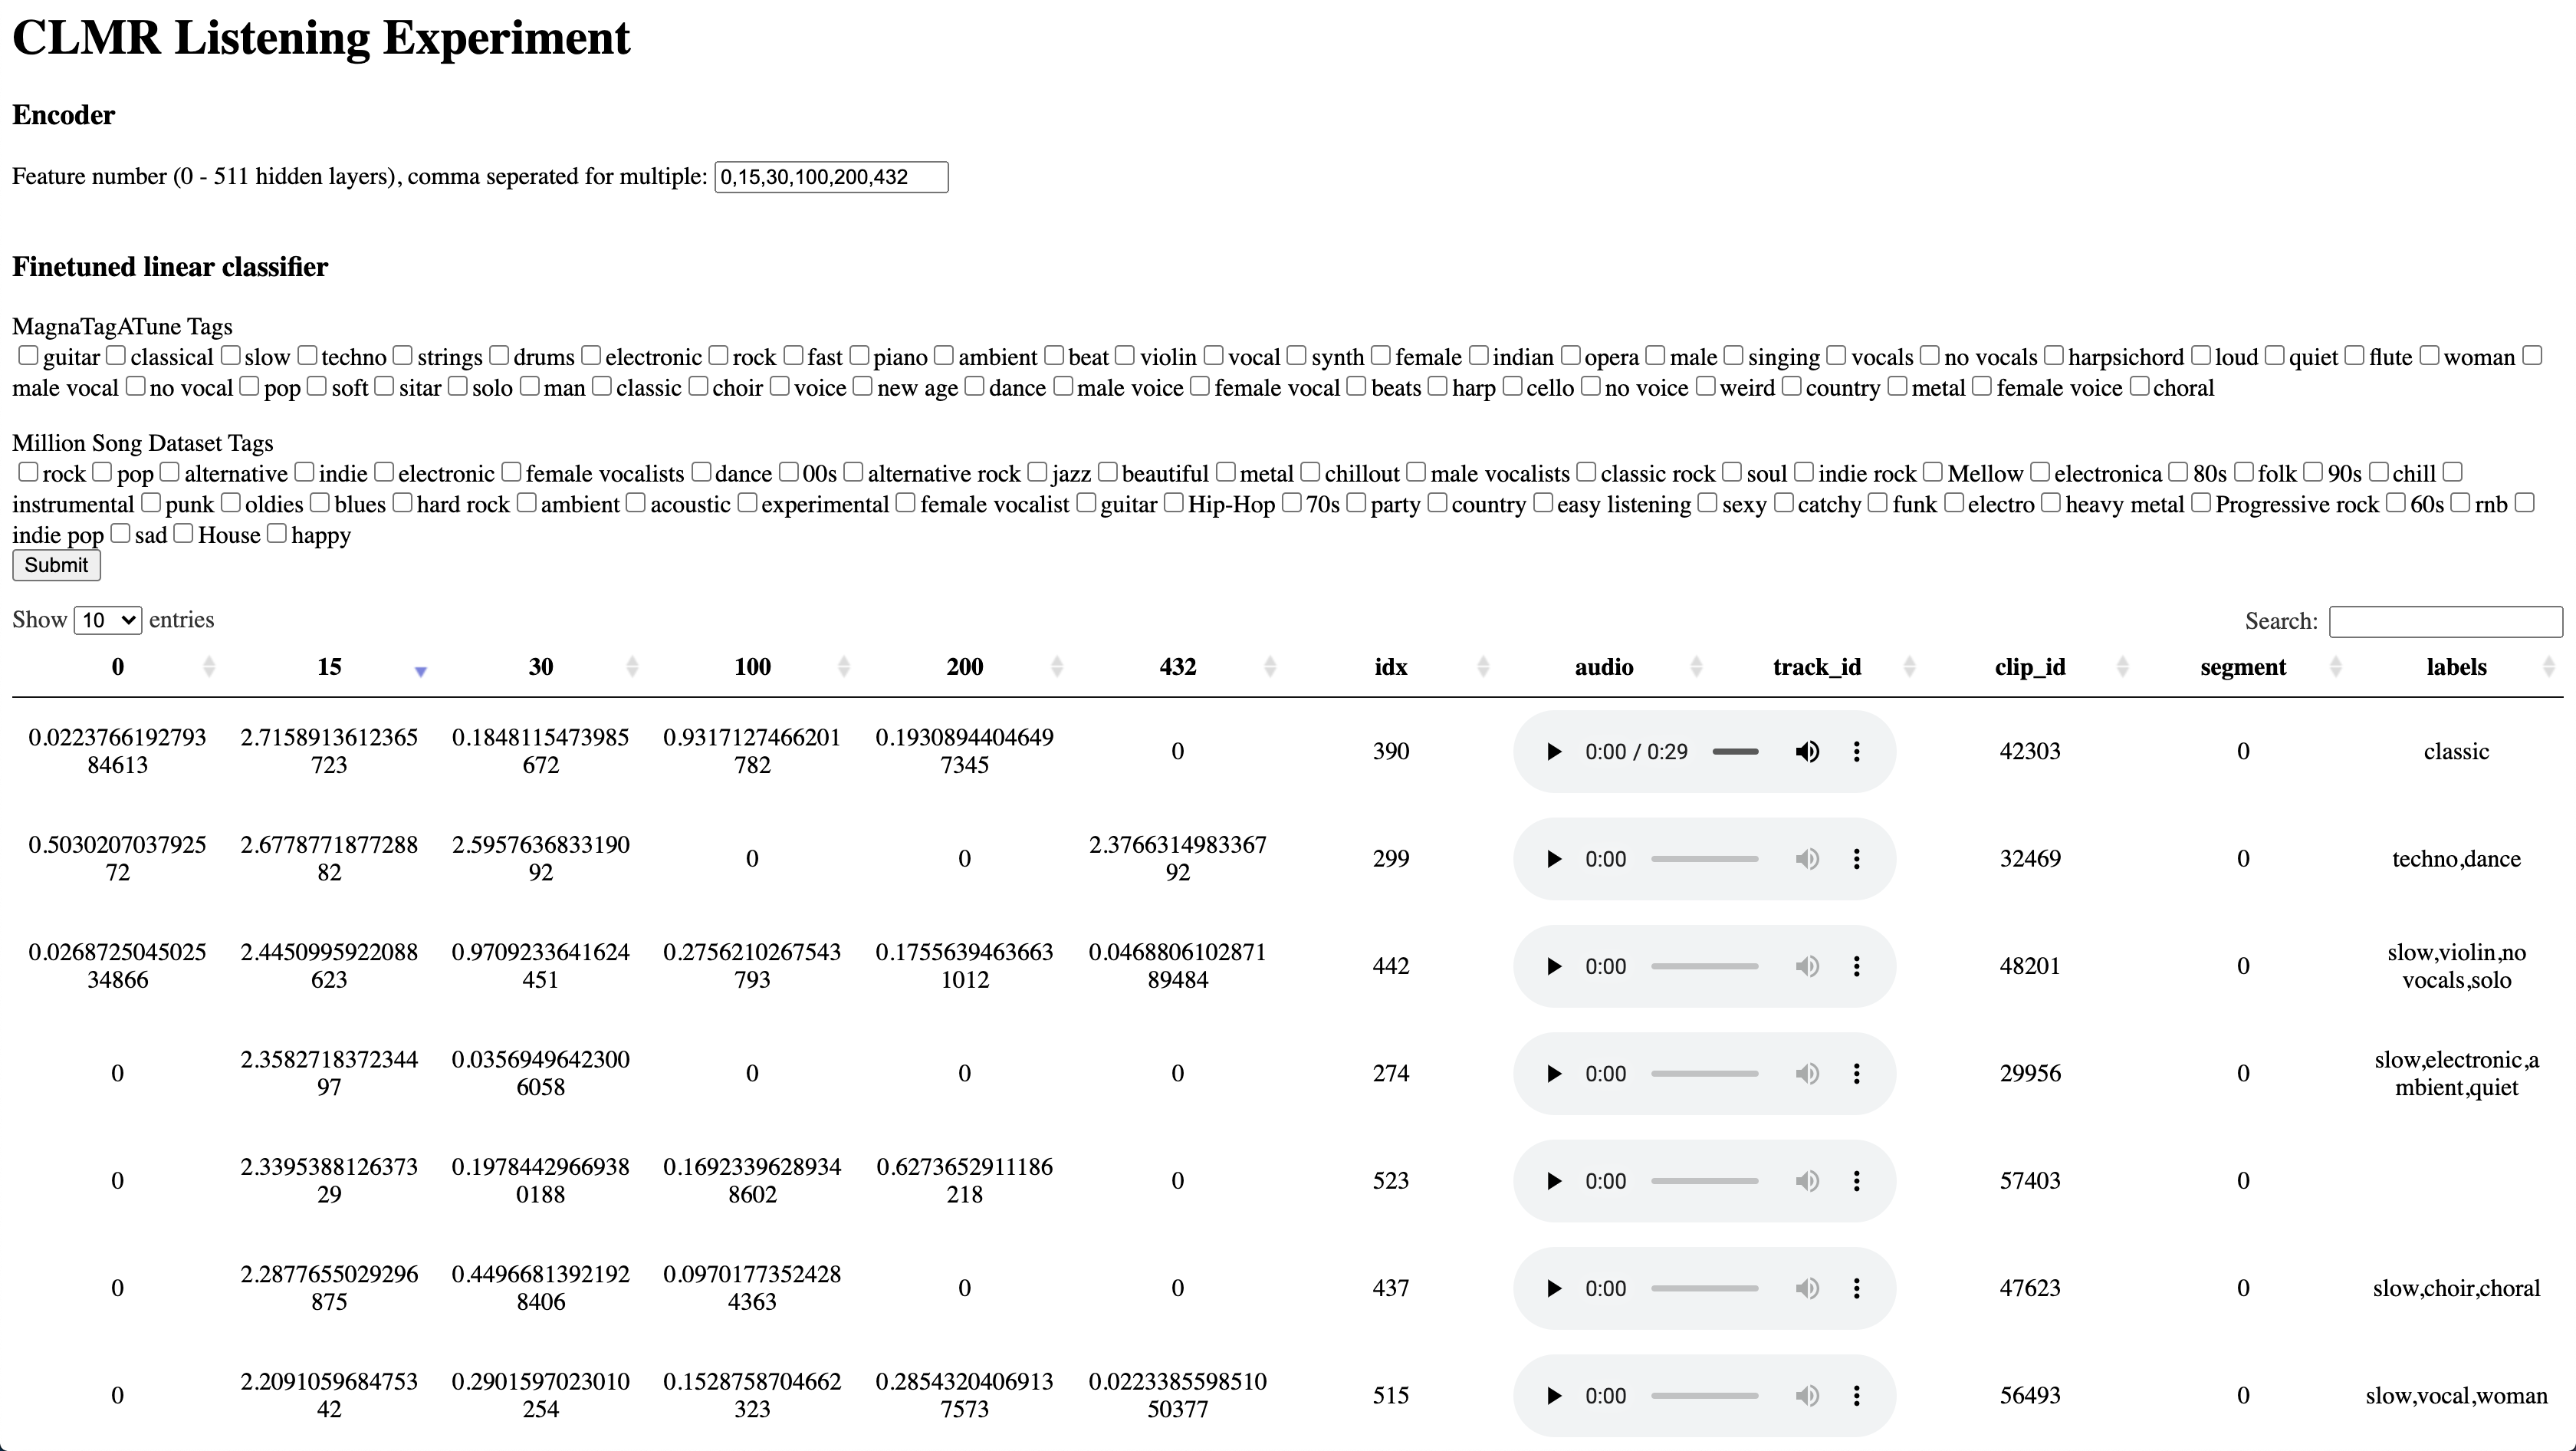
\includegraphics[width=\textwidth]{figs/listening_experiment.png}
    \caption{Screenshot of the listening experiment interface.}
    \label{fig:listening_experiment}
\end{figure*}


\begin{figure*}[h]
    \centering
    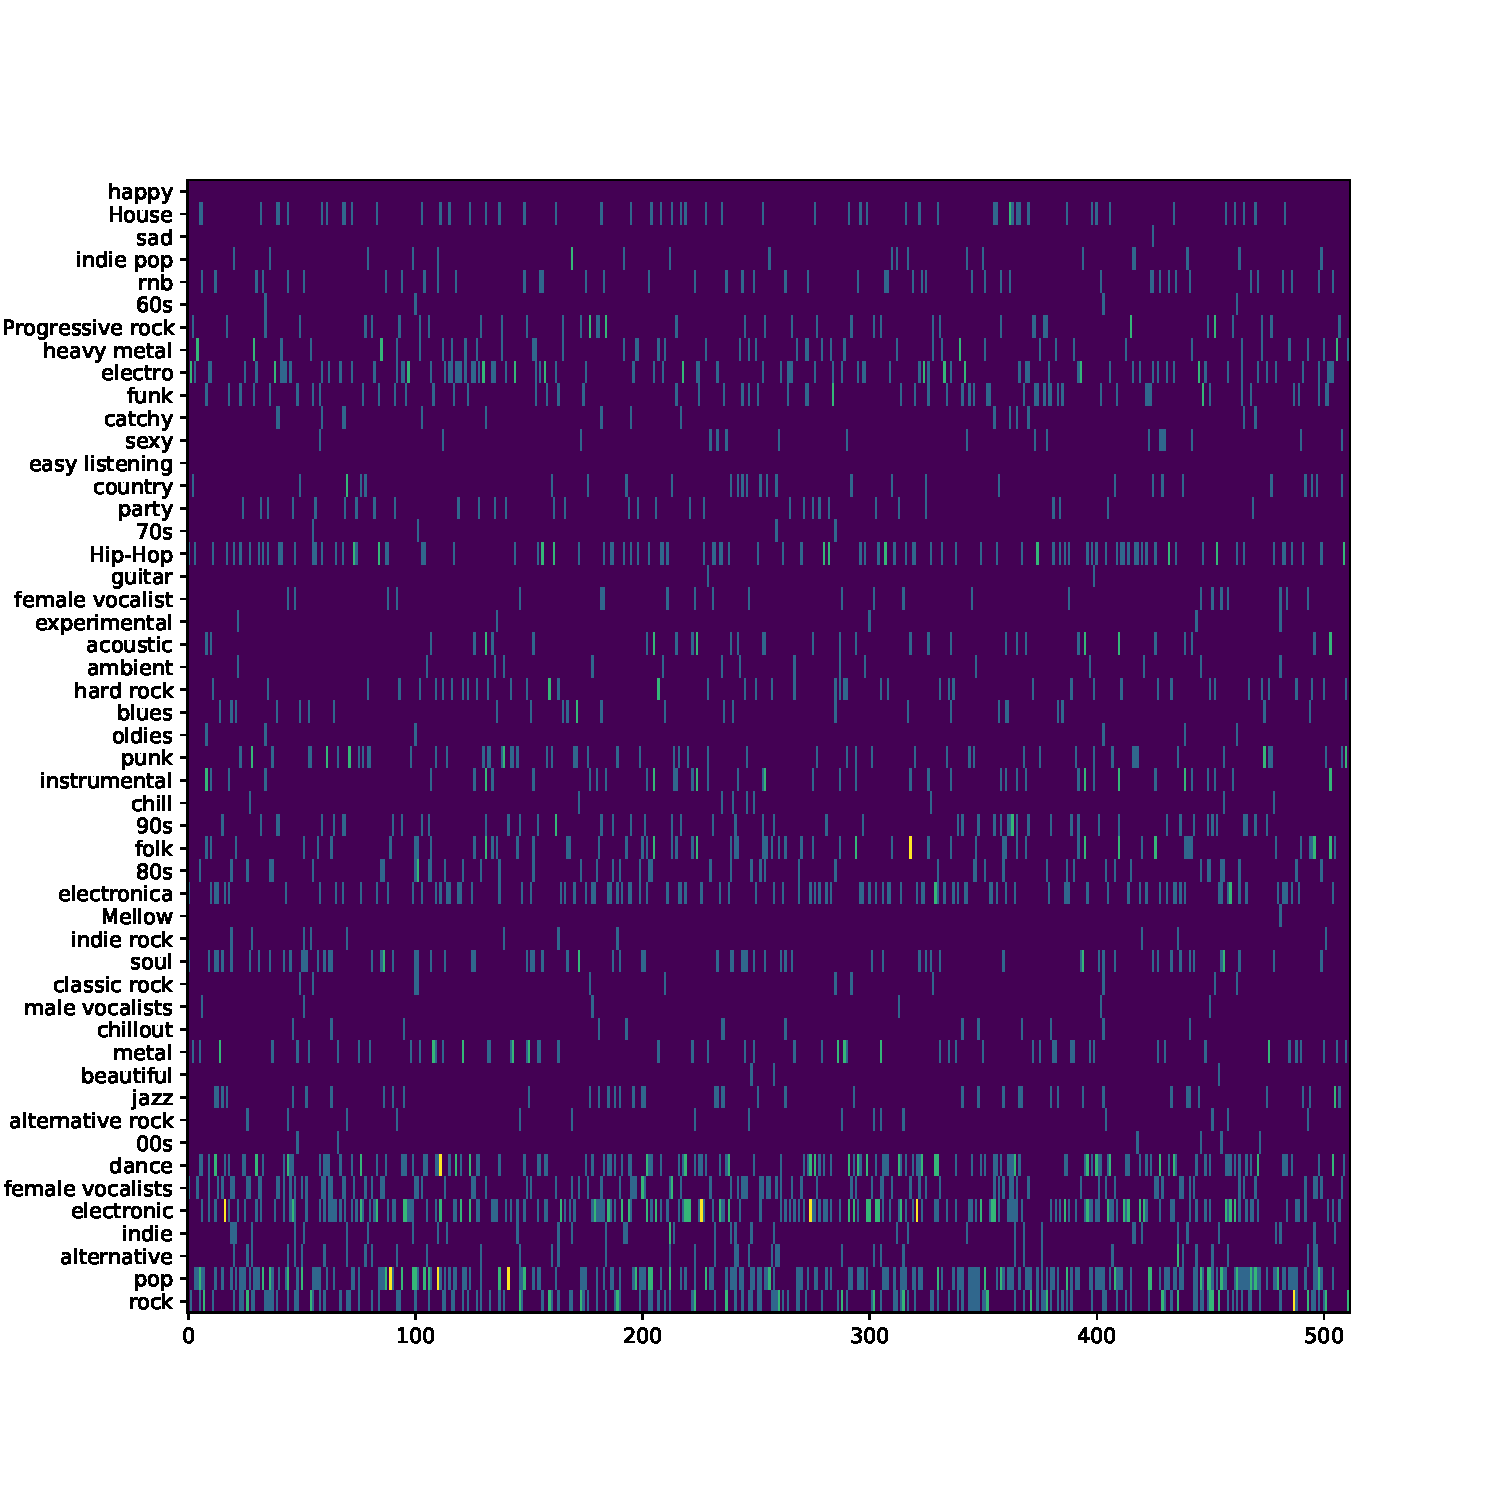
\includegraphics[width=\textwidth]{figs/features_tags_frequency.pdf}
    \caption{Occurrence of tags for the 100 most activating segments for each feature number. Purple indicates low, yellow indicates a high frequency.}
    \label{fig:tag_frequency}
\end{figure*}

\chapter{Conclusion}\label{sec:conclusion}
In this paper, we presented CLMR, a self-supervised contrastive learning framework that learns useful and compact representations of raw waveforms of musical audio.

The framework requires no preprocessing of the input and is trained without ground truth, which enables simple and straightforward pre-training on datasets of unprecedented scale, requiring no human labeling. We tested the learned, task-agnostic representations by fine-tuning a linear classifier on the music classification task on both the MagnaTagATune and Million Song Dataset, achieving state-of-the-art and competitive performance respectively. We showed that CLMR can achieve comparable downstream task performance using 100$\times$ fewer labels, and demonstrated the out-of-domain transferability of representations learned from pre-training on entirely different datasets of musical audio. We also demonstrated the out-of-domain generalisability of the CLMR model with a listening experiment.

While we hope this research will advance the field of Music Information Retrieval into a new learning paradigm, we would like to put forward the following recommendations:

\begin{itemize}
    \item Care must be taken when compiling a dataset of music for pre-training. The biases that are learned inherently in the CLMR model are not investigated in this research. These biases could lead to a potentially skewed prediction performance in favor of a select genre or type of music.
    \item CLMR requires no human-annotated labels to learn useful representations of music. While normally compensation is provided for human annotation, and, with the absence of this requirement, we recommend instead to compensate artists directly when training this algorithm on their music when developing a commercial application.
\end{itemize}

To foster reproducible research, we published the source code and pre-trained models of this research on GitHub.\footnote{\url{https://github.com/spijkervet/CLMR}}
The simplicity of training the model without a direct supervised signal and without preprocessing inputs, together with encouraging results obtained with a single linear layer optimised for a challenging downstream task, are exciting developments towards unsupervised learning on raw musical audio.

\appendix
% \begin{table*}[h]
    \centering
    \resizebox{\textwidth}{!}{
        \begin{tabular}{c|c|c|c|c|c|c|c|c|c|c|c|c}
        batch size & audio length & sample rate & projector dim. & temperature & $p_{\mathrm{invert}}$ & $p_{\mathrm{noise}}$ & $p_{\mathrm{gain}}$ & $p_{\mathrm{filter}}$ & ROC-AUC$^{(\mathrm{MLP})}$ & PR-AUC$^{(\mathrm{MLP})}$ \\ \hline
        48 & 59049 & 22050 & 128 & 0.1 & 0.8 & 0.5 & 0.1 & 0.4 & \textbf{87.56} & 32.25 \\
        48 & 59049 & 22050 & 128 & 0.5 & 0.8 & 0.5 & 0.1 & 0.4 & 87.55 & 32.66 \\
        192	& 20736 & 8000 & 128 & 0.5 & 0.8 & 0.5 & 0.1 & 0.4 & 87.52 & 32.43 \\
        48	& 20736 & 8000 & 128 & 0.5 & 0.8 & 0.5 & 0.1 & 0.4 & 87.49 & 32.38 \\
        48 & 59049 & 22050 & 256 & 0.5 & 0.8 & 0.5 & 0.1 & 0.4 & 87.43 & 32.58 \\
        48 & 59049 & 22050 & 64	& 0.5 & 0.8 & 0.5 & 0.1 & 0.4 & 87.43 & 32.49 \\
        128 & 31104 & 12000	& 128 & 0.5 & 0.8 & 0.5 & 0.1	& 0.4 & 87.41 & \textbf{32.73} \\
        48 & 31104 & 12000 & 128 & 0.5 & 0.8 & 0.5 & 0.1 & 0.4 & 87.37 & 32.69 \\
        48 & 59049 & 22050 & 128 & 0.25 & 0.8 & 0.5 & 0.1 & 0.4 & 87.36 & 32.42 \\
        48 & 59049 & 22050 & 128 & 0.5 & 0.8 & 0.5 & 0.1 & 0.4 & 87.00 & 31.93 \\
        48 & 59049 & 22050 & 128 & 0.5 & 0.8 & 0.5 & 0.1 & 0 & 85.99 & 30.26 \\
        48 & 59049 & 22050 & 128 & 0.5 & 0.8 & 0 & 0 & 0 & 85.79 & 30.55 \\
        48 & 59049 & 22050 & 128 & 0.5 & 0.8 & 0.5 & 0 & 0 & 85.67 & 30.03 \\
        48	& 59049	& 22050	& 128 & 0.5	& 0 & 0 & 0 & 0	& 85.54 & 29.84 \\
        \end{tabular}
    }
    \caption{Ablation study of CLMR under different parameters, sampling rate and data augmentations. The ROC-AUC and PR-AUC scores are obtained with a logistic regression classifier with one hidden layer, and is trained only on the representations from a pre-trained, frozen CLMR network.}
    \label{tab:1}
\end{table*}


\begin{figure*}[h]
    \centering
    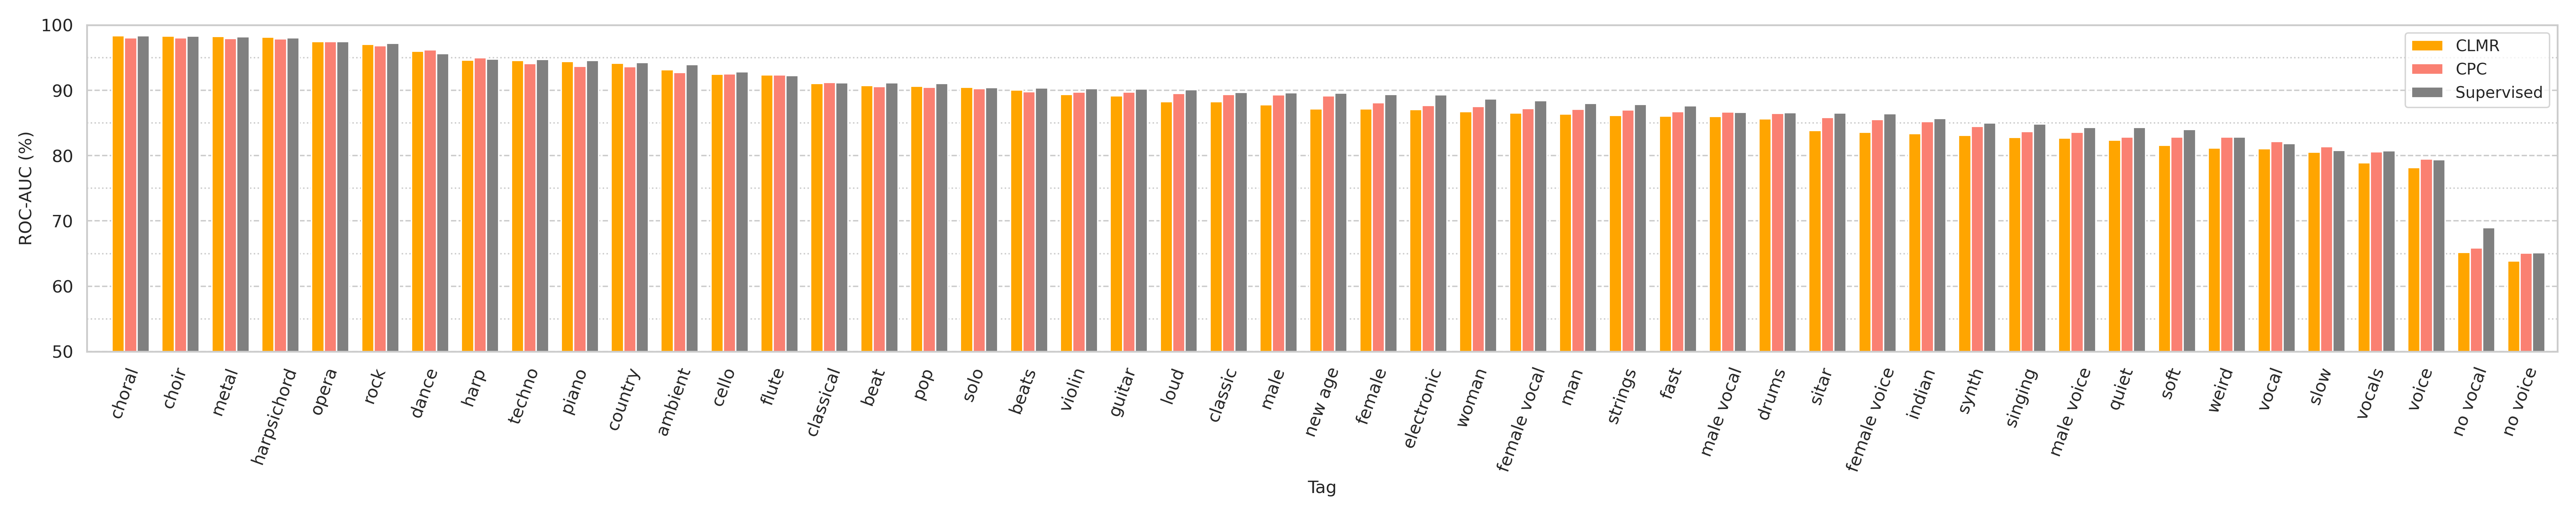
\includegraphics[width=\textwidth]{figs/tag_retrieval.png}
    \caption{Tag-wise ROC-AUC scores for the top-50 tags in the MagnaTagATune dataset, reported for linear, logistic regression classifiers trained on representations of self-supervised models CLMR and CPC, and compared to a fully supervised, end-to-end SampleCNN model.}
    \label{fig:tag_scores}
\end{figure*}



\begin{figure*}[h]
    \centering
    \subcaptionbox{CLMR$^{(1)}_{\mathrm{MTAT}}$\label{fig:1a}}{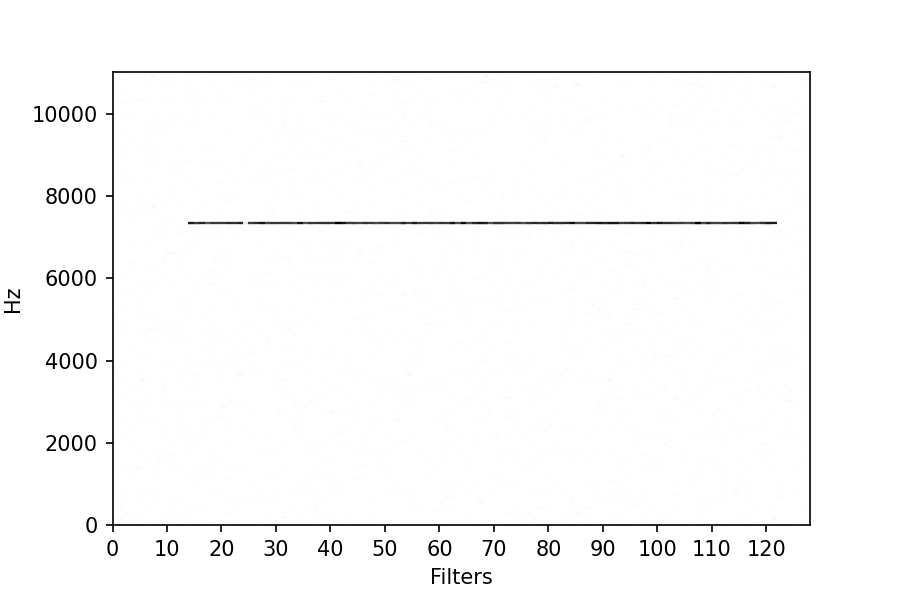
\includegraphics[width=.16\textwidth]{figs/magnatagatune/clmr_spectrum/epoch1490_layer0.png}}\hfill
    \subcaptionbox{CLMR$^{(4)}_{\mathrm{MTAT}}$\label{fig:1a}}{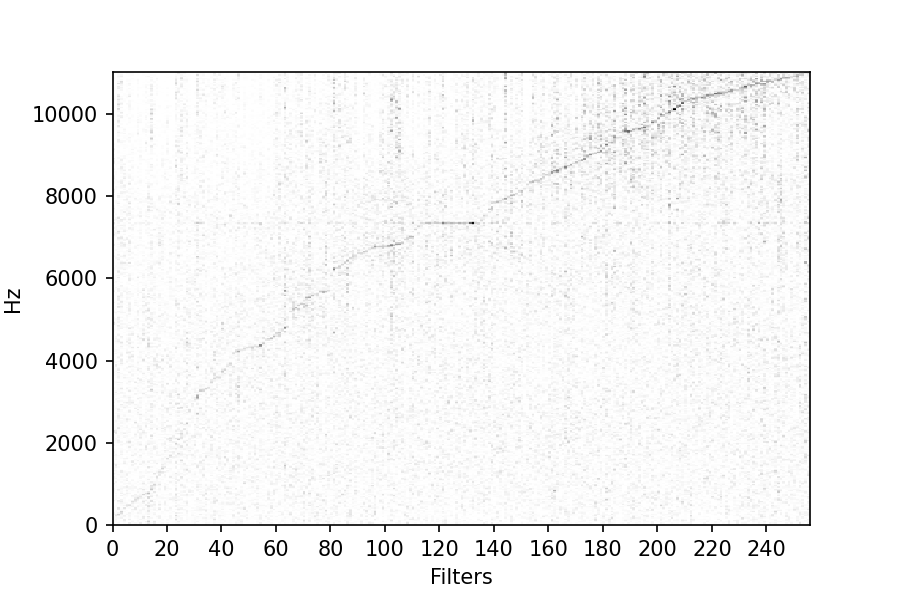
\includegraphics[width=.16\textwidth]{figs/magnatagatune/clmr_spectrum/epoch1490_layer3.png}}\hfill
    \subcaptionbox{CLMR$^{(6)}_{\mathrm{MTAT}}$\label{fig:1a}}{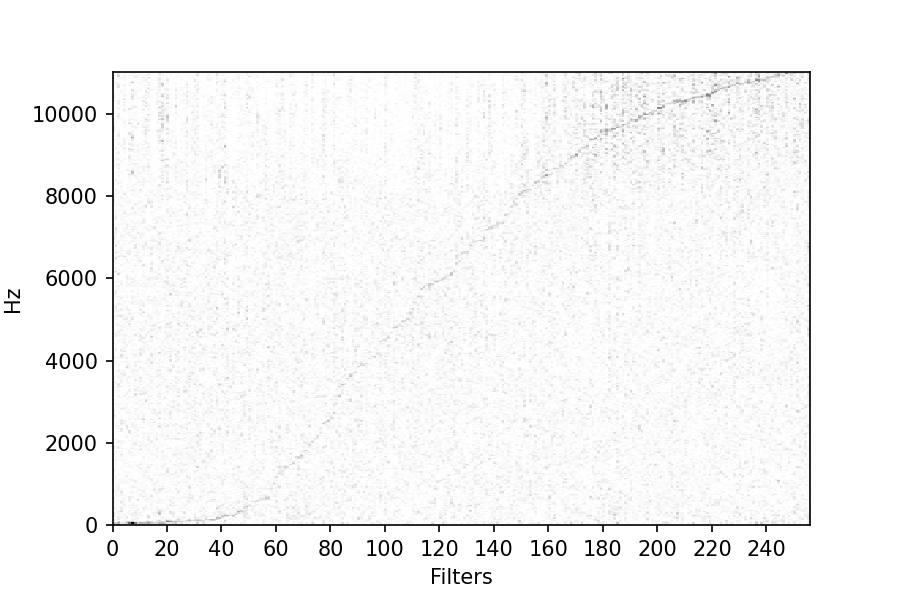
\includegraphics[width=.16\textwidth]{figs/magnatagatune/clmr_spectrum/epoch1490_layer5.png}}\hfill
    \subcaptionbox{CPC$^{(1)}_{\mathrm{MTAT}}$\label{fig:1a}}{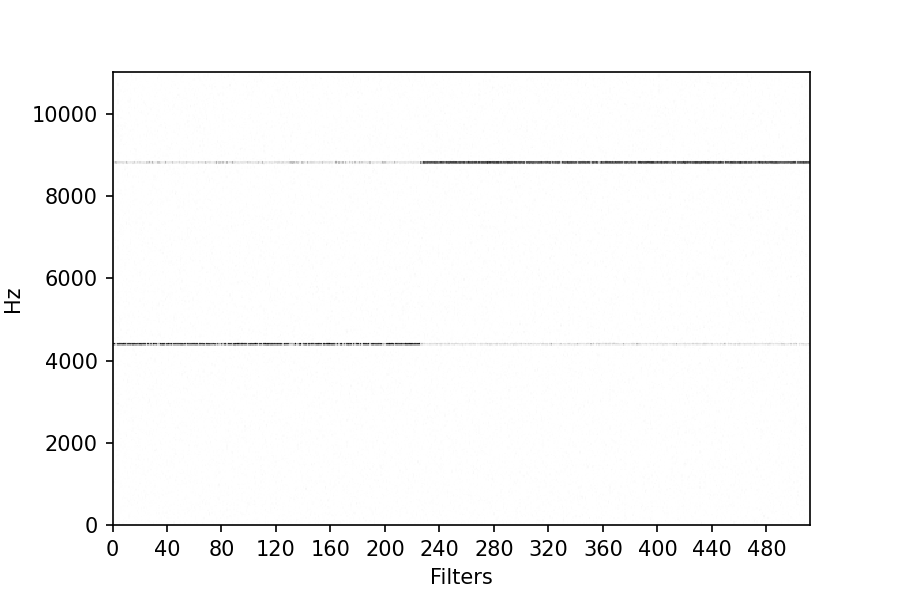
\includegraphics[width=.16\textwidth]{figs/magnatagatune/cpc_spectrum/epoch670_layer0.png}}\hfill
    \subcaptionbox{CPC$^{(4)}_{\mathrm{MTAT}}$\label{fig:1a}}{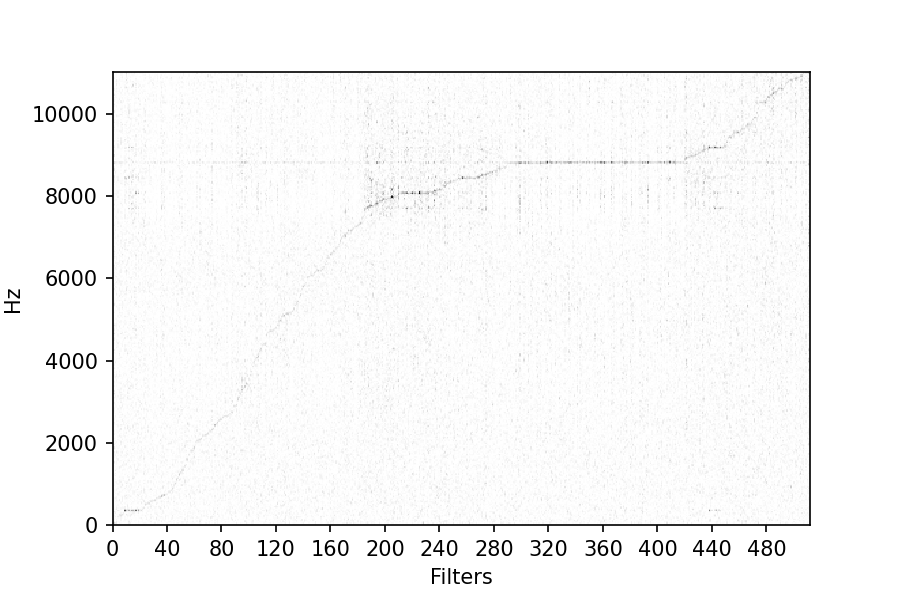
\includegraphics[width=.16\textwidth]{figs/magnatagatune/cpc_spectrum/epoch670_layer3.png}}\hfill
    \subcaptionbox{CPC$^{(6)}_{\mathrm{MTAT}}$\label{fig:1a}}{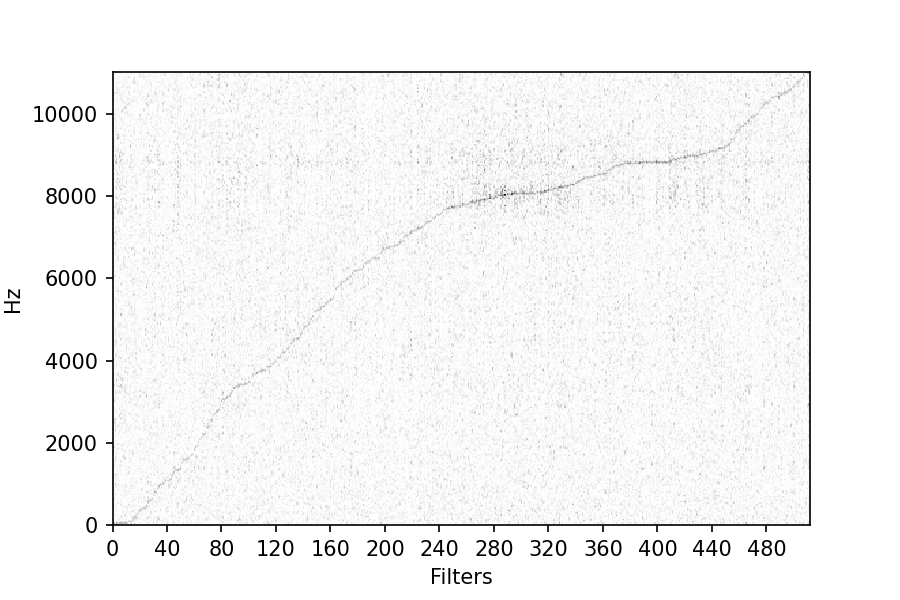
\includegraphics[width=.16\textwidth]{figs/magnatagatune/cpc_spectrum/epoch670_layer5.png}}

    \subcaptionbox{CLMR$^{(1)}_{\mathrm{Billboard}}$\label{fig:1a}}{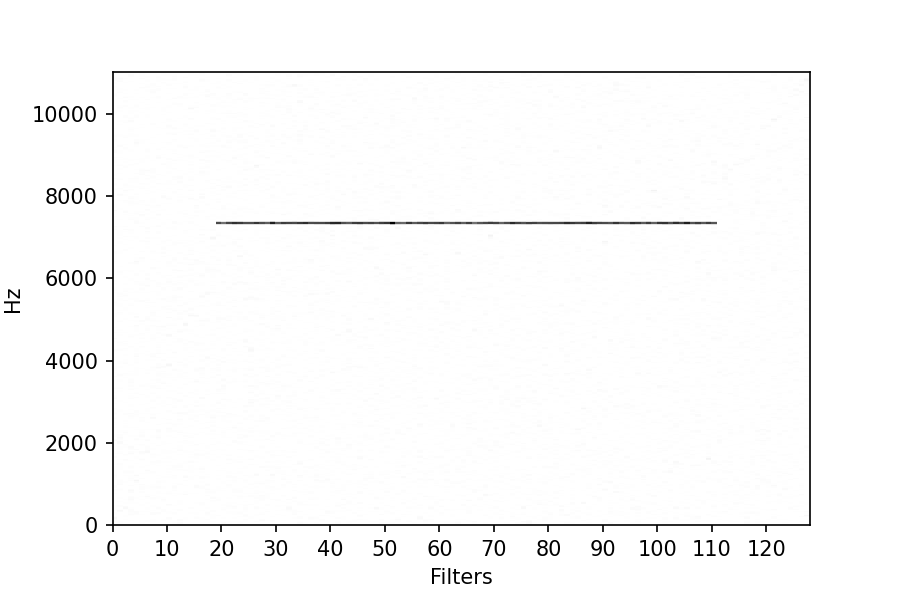
\includegraphics[width=.16\textwidth]{figs/billboard/clmr_spectrum/epoch1490_layer0.png}}\hfill
    \subcaptionbox{CLMR$^{(4)}_{\mathrm{Billboard}}$\label{fig:1a}}{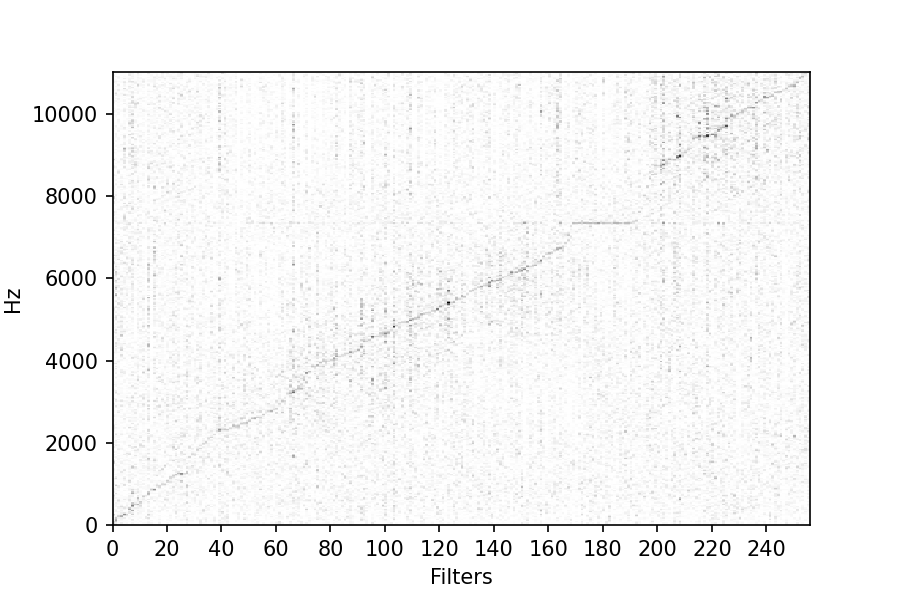
\includegraphics[width=.16\textwidth]{figs/billboard/clmr_spectrum/epoch1490_layer3.png}}\hfill
    \subcaptionbox{CLMR$^{(6)}_{\mathrm{Billboard}}$\label{fig:1a}}{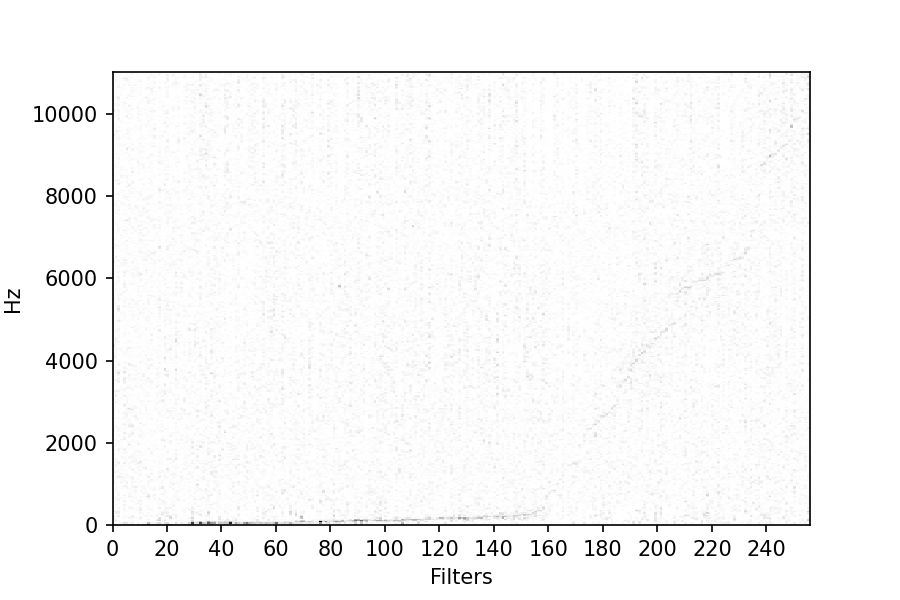
\includegraphics[width=.16\textwidth]{figs/billboard/clmr_spectrum/epoch1490_layer5.png}}\hfill
    \subcaptionbox{CPC$^{(1)}_{\mathrm{Billboard}}$\label{fig:1a}}{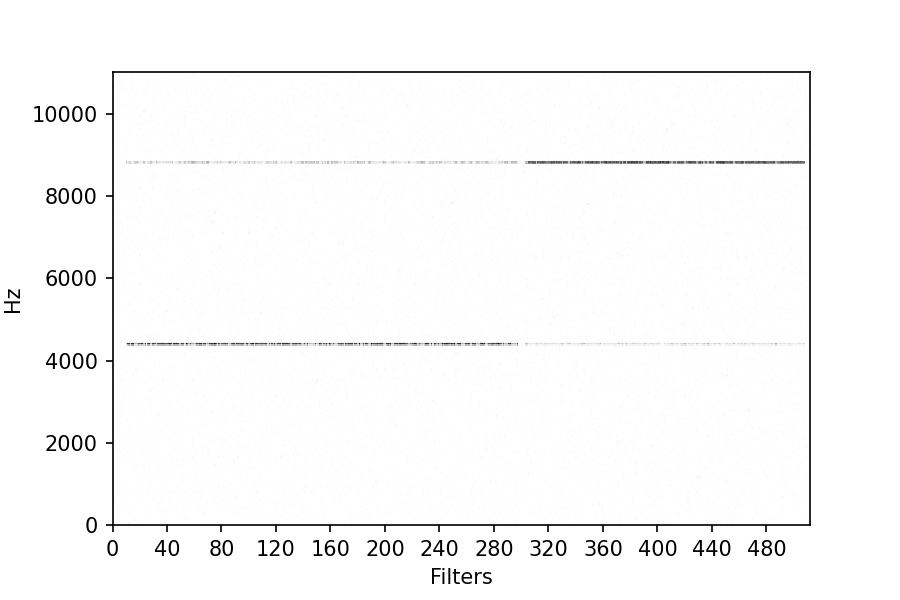
\includegraphics[width=.16\textwidth]{figs/billboard/cpc_spectrum/epoch1490_layer0.png}}\hfill
    \subcaptionbox{CPC$^{(4)}_{\mathrm{Billboard}}$\label{fig:1a}}{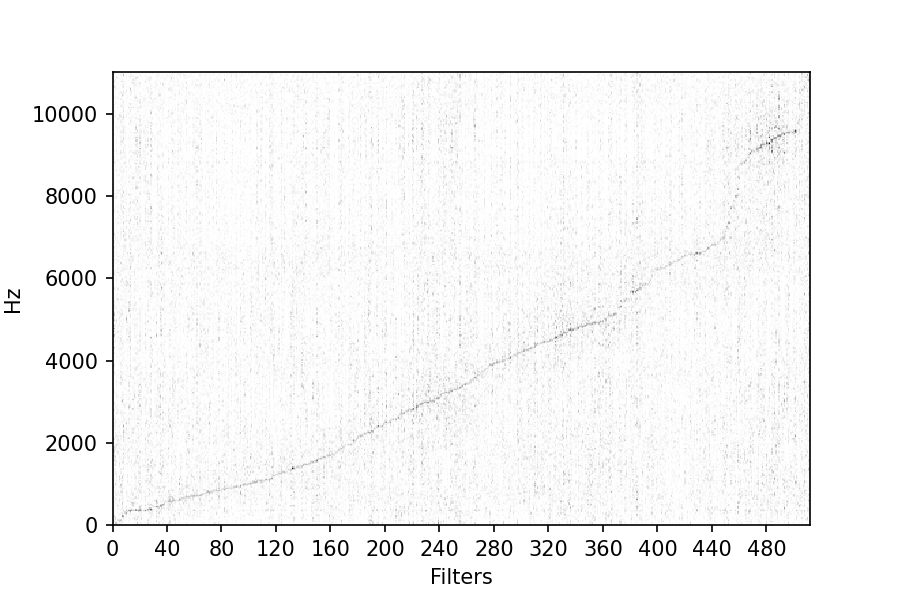
\includegraphics[width=.16\textwidth]{figs/billboard/cpc_spectrum/epoch1490_layer3.png}}\hfill
    \subcaptionbox{CPC$^{(6)}_{\mathrm{Billboard}}$\label{fig:1a}}{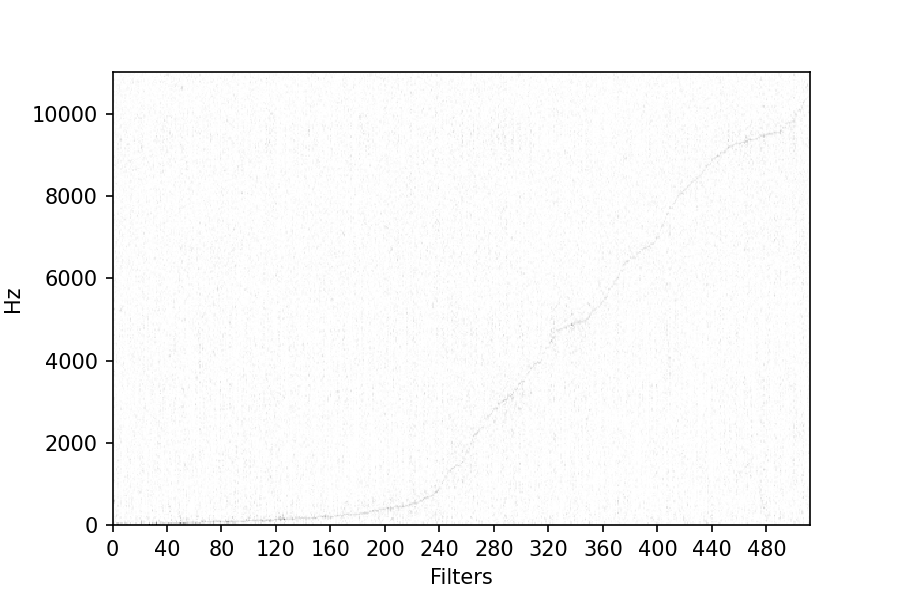
\includegraphics[width=.16\textwidth]{figs/billboard/cpc_spectrum/epoch1490_layer5.png}}

    \caption{Normalised magnitude spectrum of the filters of the self-supervised models in the sample-level convolution layers, sorted by the frequency of the peak magnitude. Gradient ascent is performed on a randomly initialised waveform of 729 samples (close to typical frame size) and its magnitude spectrum is calculated subsequently. Each vertical line in the graph represents the frequency spectrum of a different filter. The first three images are taken from a pre-trained, converged CLMR model, the last three from a CPC model, on the MTAT or Billboard datasets}
    \label{fig:filter_visualisation}
\end{figure*}

\begin{singlespace}
  \bibliography{main.bib}
  \bibliographystyle{apalike}
\end{singlespace}

\end{document}

